%------------------------------------------------------
%    PREAMBLE
%------------------------------------------------------
% --- DOCUMENT CLASS
\documentclass[
DIV=calc,
a4paper,
fontsize=12pt
]{scrreprt}   % 'report'-class is used, alternatives: 'scrreprt' (see: https://www.ctan.org/pkg/scrreprt)
% Check this page: https://www.overleaf.com/learn/latex/Sections_and_chapters


% --- Packages
\usepackage[utf8]{inputenc}
\usepackage{hyperref}
\usepackage{graphicx}   % Required for inserting images
\usepackage{minted}     % Required for code blocks (i.e. Python)
\usepackage{geometry}   % Required for page layout
\usepackage{scrhack}    % To avoid warnings on floating
%\usepackage{wrapfig}    % To wrap math formulas around a figure
\usepackage{mathtools}
%\usepackage{amsmath}
\usepackage{glossaries}
\usepackage{subcaption}

\hypersetup{
    colorlinks=true,
    linkcolor=black,
    filecolor=blue,
    urlcolor=blue,
    citecolor=blue,
    pdftitle={Master-Thesis Rainer Gogel},
    pdfpagemode=FullScreen,
    }

\loadglsentries{Chapters/0_Glossary.tex}
\makenoidxglossaries

%------------------------------------------------------
%    LAYOUT AND STYLE
%------------------------------------------------------

% Global settings for package 'minted'. Python 'styles' available in Pygment: https://pygments.org/styles/
\setminted[python]{
style=default,
fontsize=\scriptsize,
frame=lines,
framesep=2mm,
linenos=true,
baselinestretch=1.2,
breaklines=true
}

% This changes the name from "Listing ..." to "Python Code ..."
\renewcommand{\listingscaption}{Python-Code}
% --- Layout
% \newgeometry{
% top = 3cm,
% bottom = 3cm,
% outer = 3cm,
% inner = 3cm
% }

%------------------------------------------------------
%    FIRST PAGE
%------------------------------------------------------
\titlehead{\centering
\includegraphics[width=0.25\textwidth]{Assets/uasfra-logo}\\[0.2cm]Department of Computer Science}
\subject{Master-Thesis}
\title{\Huge \emph{Constructing a Knowledge Graph by extracting information from financial news articles}}
\author{\textbf{Rainer Gogel}\\ \normalsize{Student-ID: 1272442} \\[2cm]{Advisor: Prof. Dr. Joerg Schaefer}\\{Co-Advisor: Prof. Dr. Baris Sertkaya}\\[3cm]}

\date{\today}

\begin{document}

\maketitle


%------------------------------------------------------
%    CONTENT-INTRO
%------------------------------------------------------

\chapter*{Statutory Declaration}
I herewith declare that I have completed this Master-Thesis independently, without making use of other than the specified literature and aids.
All parts that were taken from published and non-published texts either verbally or in substance are clearly marked as such.
This thesis has not been presented to any examination office before.\\


Frankfurt am Main, November 10, 2024\\


Rainer Gogel\\



\begin{figure}[H]
	
\includegraphics[width=0.3\textwidth]{Assets/signature}
\end{figure}
Signature

\chapter*{Acknowledgements}
I would like to express my sincere gratitude to Professor Dr. Joerg Schaefer and Professor Dr. Baris Sertkaya for their willingness to supervise this Master-Thesis.
I am particularly grateful to Professor Dr. Joerg Schaefer for stepping in as my primary supervisor at short notice, enabling me to escape an unpleasant situation.\\

I am also grateful to them for being a part of my academic journey and for their guidance along the way.
Their expertise, passion for their field, and dedication to imparting knowledge through insightful and inspiring lectures and exercises have significantly enriched this journey.
I am truly grateful for the wonderful learning experience they have provided.

\chapter*{Summary}
Reading and understanding news articles takes time and effort and some readers are only interested in information that is relevant to them.
This Master-Thesis project demonstrates how a user, who is only interested in news about certain companies and topics, can retrieve such information from financial news articles in an efficient manner.\\

The project’s code extracts company names and their \gls{coref_definition} from the news text, classifies this text into different topic classes and stores this information in a Knowledge Graph.
This way, the user can retrieve the desired information and discover complex relationships by querying the Knowledge Graph or by communicating with the Knowledge Graph’s ChatBot (\gls{graph-bot}).\\

In the \emph{Information Extraction Pipeline}, different approaches were studied, implemented in code and compared with each other.
One of the key findings was that \glspl{gen-llm} can be used for a wide range of extraction tasks and that these models often outperform other, more traditional approaches.\\

Another key finding is that the retrieved information from the \gls{graph-bot} should also be more accurate than answers coming from a typical \gls{llm} ChatBot, even if that \gls{llm} ChatBot has a traditional \gls{RAG} system attached to it.
This is because the \gls{graph-bot}’s response is more based and focused on the stored news articles in the Knowledge Graph and less on next-word probabilities and vector similarities.\\

Such a Knowledge Graph can be seen as an alternative \gls{RAG} system that might replace the more commonly used vector databases there.
This is supported by a recently published and influential research paper by Microsoft \cite{graphrag} that points in the same direction.

%\listoffigures
\printnoidxglossaries

\tableofcontents

%------------------------------------------------------
%    CONTENT-CHAPTERS
%------------------------------------------------------

%\mainmatter % Starts regular arabic page numbering
%\include{Chapters/0_Summary}


\chapter{Introduction}\label{ch:introduction}
\section{Overview}
The goal of this Master-Thesis project is to extract structured information from unstructured text and store this information in a Knowledge Graph to facilitate information retrieval.
The unstructured text are financial news articles and the target information to be extracted is information about certain corporate entities or companies.

To extract the information, an \emph{Information Extraction Pipeline} is built that contains three main components:

\begin{figure}[H]
	\centering
	
\includegraphics[width=1.0\textwidth]{Assets/pipelineAll}
	\caption{Information Extraction Pipeline}
	\label{fig:infoextract}
\end{figure}


\begin{itemize}
	\item \textbf{NER}: A Named Entity Recognition component that identifies the desired company names in the text
	\item \textbf{Coreference Resolution}: A \gls{coref_resolution_definition} component that detects references to previously identified company names
	\item \textbf{Topic Modelling}: A Topic Modelling component that classifies those sentences in the text, that contain company names and their coreferences, into different topic classes
\end{itemize}

The \emph{Information Extraction Pipeline} yields sentences that contain company names, their \glspl{coref_definition} and the respective topic for each of these sentences.
This information is then stored in a neo4j \cite{neo4j} Graph database according to the following schema:

\begin{figure}[H]
	\centering
	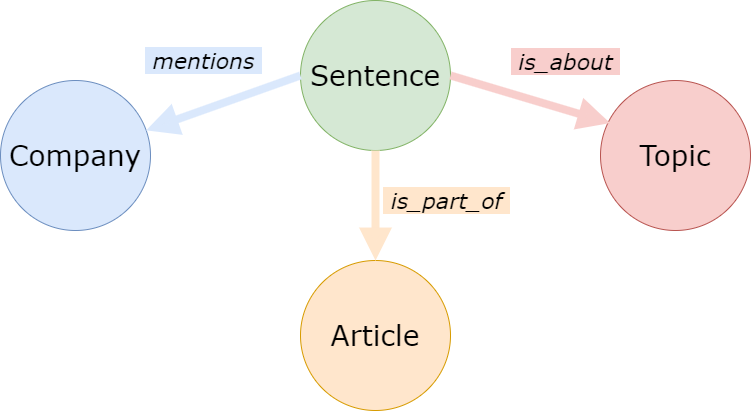
\includegraphics[width=0.85\textwidth]{Assets/kg_schema}
	\caption{Knowledge Graph Schema}
	\label{fig:kg-schema}
\end{figure}

There are three Node types in the Knowledge Graph:

\begin{itemize}
	\item \textbf{Sentence}: the \emph{Sentence} in which a \emph{Company} is mentioned
	\item \textbf{Topic}: the \emph{Topic} or overarching theme of this \emph{Sentence}
	\item \textbf{Company}: the \emph{Company} entity whose name is mentioned in the \emph{Sentence}
	\item \textbf{Article}: the \emph{Article} of which the \emph{Sentence} is part of
\end{itemize}

A \emph{Sentence} Node thus has three relationships to other Nodes in the Knowledge Graph:

\begin{itemize}
	\item \textbf{is\_about}: a \emph{Sentence} is about a certain \emph{Topic}
	\item \textbf{is\_part\_of}: a \emph{Sentence} is part of an \emph{Article}
	\item \textbf{mentions}: a \emph{Sentence} mentions a \emph{Company}
\end{itemize}

This structured representation of the unstructured text does not only allow for fast retrieval of concrete information, but can also reveal complex relationships between multiple companies, topics and articles.

The stored information can be retrieved via \gls{cypher} queries that can also be generated by an \gls{llm}-based \gls{graph-bot} that first converts human text to \gls{cypher} queries and then the results back to human-readable text.

\section{Thesis and Code}\label{sec:domain-focus}
This Master-Thesis consists of two separate parts, the written thesis and the accompanying Python code.

\paragraph{Python Code}
The Python code can be found in the following GitHub repository:
\begin{center}
	\textbf{\url{https://github.com/rainergo/UASFRA-MS-Thesis}}
\end{center}
The code could be used as a template for a production use case, but mainly serves to support this Master-Thesis and to present the process rather than the result.\\
All functionalities of the code are aggregated and condensed in the Jupyter Notebook
\begin{center}
	\emph{MAIN.ipynb}
\end{center}
located in the root directory of the repository and explained in Appendix \ref{ch:explanation-of-main-file}.
This Notebook runs the entire pipeline from text to Knowledge Graph.

\paragraph{Target Use Case}
The Python code is targeted at a user with a particular focus on financial news of publicly listed European companies in German language.
This focus is driven by my professional background in finance and personal interest in this field.

\section{Thesis Outline}\label{sec:thesis-outline}
This thesis will be divided into multiple chapters.
In the chapter after this introduction, I describe the source and nature of the text data.\\
Thereafter, I will describe the spacy \cite{spacy} Python library and how it was used, followed by an introduction to text representation.\\
In the fourth chapter, I start with a description of Named Entity Recognition (\gls{ner}) and how that pipeline component was implemented in code.\\
The same approach applies to the \gls{coref_resolution_definition} and Topic Modelling chapters thereafter.\\
In the Knowledge Graph chapter, I show how the previously extracted data is fed into the neo4j database and how information retrieval algorithms can reveal some complex relations between news articles, companies and topics.\\
I conclude with what I learned from this project and where in hindsight I would approach tasks differently.
\chapter{Project Setup}\label{ch:project_setup}
This chapter will describe the project's data sources and the Python library \emph{spacy}, which was extensively used for the \gls{ner} and \gls{coref_resolution_definition} components in the \emph{Information Extraction Pipeline}.

\section{Data}\label{sec:data}
The data consists of \emph{News Articles} and \emph{Company Data}.
The dataset requirements are derived from the project's domain focus as outlined in section \ref{sec:domain-focus}.
This requires that
\begin{itemize}
	\item news articles must be in German language.
	\item news articles should mention companies, at least potentially.
	\item companies must be publicly listed on a stock exchange.
	\item companies must be based in Europe.
    \item such company and news articles data must be publicly available.
\end{itemize}

\subsection{News Articles}
Many news article datasets are available on platforms such as Kaggle \cite{kaggle}, but it seems that only a few of them are in German \cite{kaggle}.
Most of the German news datasets that I analyzed are either not rooted in the financial domain, outdated for copyright reasons or
deal with macroeconomic policies or broader economic trends rather than company news.\\

As I could not find proper data that fits the outlined objectives, I decided to scrape the information from financial news providers.

\paragraph{Sources}\label{par:sources}
The data was scraped from the websites of \emph{EQS-News} \cite{WebsiteEQSNews} and \emph{dpa-AFX} \cite{WebsiteDPAAFX}, both business news hubs that aggregate multiple news sources.
The text in the html-files were converted to text files, cleaned and read into pandas \cite{pandas} DataFrames.
The type of the news articles includes \emph{ad-hoc news}, \emph{press releases}, \emph{corporate news} and \emph{regulatory filings}.
These could be published by \emph{companies} themselves or \emph{media outlets} such as newspapers, news agencies or other broadcasters.

\paragraph{Data Description}\label{par:data-description}
Of the news articles, the article text, the article title and some other metadata such as publication dates, authors, etc. were scraped.
The news articles contained many irregularities, errors, misspellings and phrases that were not part of the actual news.\\
Multiple regular expression (\gls{Regex}) patterns and techniques were applied to clean the text.
Most of the errors and undesired phrases of the text could be removed, but not all.
So the subsequent models must handle them.\\
The news article dates range from \emph{May 1, 2023} through \emph{May 31, 2024} and its frequency is daily.
The daily data was aggregated on a monthly basis and the pandas DataFrames were stored as Apache parquet \cite{parquet} files.

\subsection{Company Data}
OpenBB \cite{openbb} is an open source framework that aspires to replicate the functionalities of the Bloomberg Terminal, a costly financial service product by the media company Bloomberg \cite{bloomberg}.
OpenBB offers a wide range of functionalities, connects data providers and is the data source for the company data used in the project.
Data for companies, that are publicly listed on bourses in
\begin{itemize}
    \item France
    \item Germany
    \item Great Britain
    \item Spain
    \item Italy
    \item The Netherlands
\end{itemize}
and that are members of the main stock indexes there, were downloaded and stored in an Apache parqet file.
This file contains unique company names and their stock ticker symbols for slightly above 2500 companies.

\section{Spacy}\label{subsec:spacy}
Spacy \cite{spacy} is a modular, open-source Python library that is commonly used for a wide range of \gls{nlp}-related tasks.
For popular languages like English and German, spacy offers pre-trained pipelines (see Fig.\ref{fig:spacy-pipeline}) in different sizes and versions.
\begin{figure}[H]
	\centering
	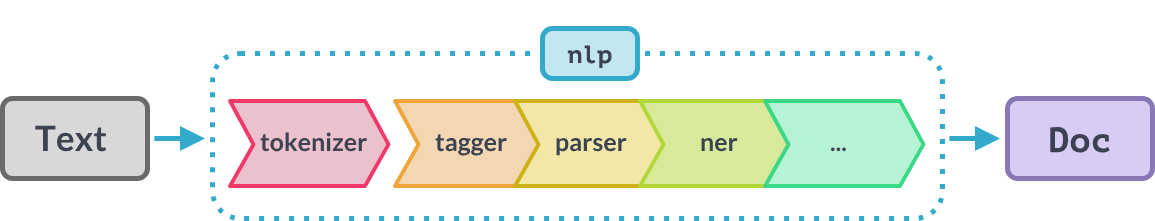
\includegraphics[width=1.0\textwidth]{Assets/spacypipe}
	\caption{\textit{Spacy Pipeline}}
	\label{fig:spacy-pipeline}
\end{figure}

The model sizes range from \emph{Small} to \emph{Medium} and \emph{Large}, with bigger models usually performing better than smaller ones.

The spacy-trained Transformer model for English is based on \gls{ROBERTA} \cite{roberta}, the one for German on \gls{BERT}-German \cite{BERT}.
The TOK2VEC \cite{spacy} embeddings for the non-Transformer models (suffixes: sm, md, lg) are memory-efficient Multi-Hash embeddings \cite{spacyembeddings} with a \gls{cnn} encoding layer \cite{spacy}.

\paragraph{Pipeline Components}
After downloading the models, by default, the modular pipeline consists of a:

\begin{itemize}
  \item \textbf{Tokenizer}: Segments text into tokens
  \item \textbf{POS-Tagger}: Assigns \gls{pos} tags such as \textit{NOUN} or \textit{VERB}
  \item \textbf{Dependency-Parser}: Assigns syntactic dependency labels between \gls{pos}-tags and sets sentence boundaries
  \item \textbf{Lemmatizer}: Assigns base forms or lemmas (see: \gls{lemmatization})
  \item \textbf{Entity-Recognizer}: Detects and labels named entities such as \gls{org} or \gls{per}
  \item \textbf{Custom Components}: Proprietary components implemented by the user
  \item \textbf{Pipeline Plugins}: External applications that are developed by others as a spacy pipeline component
\end{itemize}

The \emph{Dependency-Parser} and \emph{Entity-Recognizer} modules in the pipeline were separately trained with task-specific datasets and plugged back into the pipeline \cite{spacy} (see Fig.\ref{fig:spacy-pipeline}).

\paragraph{Custom Component}
With a spacy \emph{Custom Component}, users can implement their own custom algorithms and functions.
Compared to a pure Python implementation, these \emph{Custom Components} are usually faster as they are optimized with \gls{CPython} in the background.
This functionality was extensively used in the project as the \gls{ner} and \gls{coref_resolution_definition} pipeline components (see Fig.\ref{fig:infoextract}) were implemented with such \emph{Custom Components}.

\paragraph{Pipeline Plugins}\label{par:spacy-plugin}
Spacy \emph{Pipeline Plugins} are applications and standalone packages that are developed by other software developers to be used as a spacy pipeline component.
Such registered plugins enhance the spacy ecosystem and can easily be added by referencing it in the \textit{add\_pipe()}-function.
One such plugin studied in the project is the package \emph{Crosslingual-Coreference} ("xx\_coref") \cite{xxCoref} that was loaded with the
\begin{center}
\emph{nlp.add\_pipe("xx\_coref")}
\end{center}
function.

\paragraph{Custom Extensions}
Users can also attach custom extensions to spacy's \glspl{token} and \glspl{span} in a \emph{Doc}-Object (see Fig.\ref{fig:spacy-pipeline}) which allows them to tag or label certain words or expressions in the text to further process them later.
In the project, such custom extensions were also used extensively.
For instance: For a company identified in the \gls{span} or \gls{token} of a document (\emph{Doc}-object), the company name and company symbol (stock tocker symbol) were attached to the custom extensions \emph{comp\_name} and \emph{comp\_symbol} as in the following example:

\begin{center}
    \emph{doc.\_.comp\_name = "Adidas AG"}
\end{center}
\begin{center}
    \emph{doc.\_.comp\_symbol = "ADS.DE"}
\end{center}

Later on, all companies in a \textit{Doc}-object can be collected and further processed.

\paragraph{Modularity and Custom Pipeline}
The \emph{Tokenizer}-component is always required in the pipeline, but all other components (see Fig.\ref{fig:spacy-pipeline}) can easily be removed from it if they are not needed for a specific \gls{nlp}-task.
For instance, if only a \gls{pos}-tagger is needed to identify \emph{Nouns}, it can be enabled with the \emph{select\_pipes()}-method which also disables all other components except for the \emph{Tokenizer}:

\begin{center}
\emph{nlp.select\_pipes(enable="tagger")}
\end{center}

\subsection{Usage}\label{subsec:usage}
The spacy \emph{Custom Pipeline} was build with Python modules that can be found in the following directory:
\begin{center}
    \emph{src/B\_spacy\_pipeline}
\end{center}
In the \emph{spacy\_pipe\_build} module and \emph{SpacyPipeBuild} class, the method \emph{build\_pipe()} (Python-Code \ref{code:build-pipe}) controls the pipeline's components:

\begin{listing}[H]
    \captionof{listing}{Function: build\_pipe()}
    \inputminted[
    firstline=60,
    lastline=81,
    firstnumber=60,
    ]{python}{/media/rainergo/PROJECTS/UASFRA-MS-Thesis/src/B_spacy_pipeline/spacy_pipe_build.py}
    \label{code:build-pipe}
\end{listing}

A pipeline component can be replaced by substituting it with the desired module function depending on the specific task.
All module functions are defined in the \emph{SpacyPipeBuild} class.

\paragraph{Other Python Libraries}
Beside spacy, other important Python libraries were used, but these will be described within their particular scope in the subsequent chapters.




\chapter{Text Representation}\label{ch:text-representation}

\section{Overview}\label{sec:overview_text_representation}
The key question in text processing and \gls{nlp} is how to encode text into numbers so that computers can understand them.
The process is also known as \emph{Vectorization} \cite{word2vec2} and there are two main approaches to vectorize text.\\
The first and more traditional approach is to encode word or \gls{token} occurrence counts.
A more modern approach is to train Artificial Neural Networks (\gls{ann}) to get text embeddings that also incorporate syntax and semantics.
In the next subsections, I will explain these encoding techniques as they form the foundation for most of the subsequent chapters.


\section{Definitions}\label{sec:definitions}
In \gls{nlp}, the terms \gls{corpus}, \gls{vocabulary} and \gls{document} are often interpreted differently which requires clarification.
In this thesis, a \gls{document} is defined as text that might contain multiple sentences such as a news article in the data described above.
All news articles in the entire data set constitute the \gls{corpus} which refers to a collection of documents.
All unique words in a \gls{corpus} represent the \gls{vocabulary}.
A \gls{document_term_matrix} is a tabular data structure where rows represent references to documents and columns represent the unique terms of a vocabulary.
Such terms or \glspl{token} can either be words or sub-words and in a \gls{document_term_matrix} represent its features.
The data entries in the \gls{document_term_matrix} are the feature values and show if or how often the term appears in the respective document.

A simplified example can be seen in Fig.\ref{fig:sample_docs} and in Fig.\ref{fig:document_term_matrix}:

\begin{figure}[H]
    \centering
    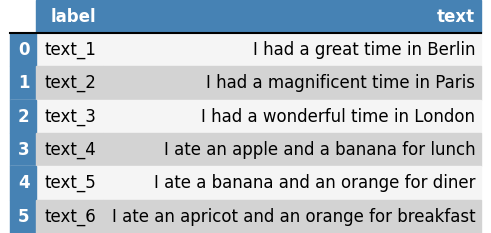
\includegraphics[keepaspectratio=true,scale=0.6]{Assets/topic_model_text}
    \caption{Sample Documents}
    \label{fig:sample_docs}
\end{figure}

The text in each row is a \gls{document} though in this example only contains one sentence each and
the \gls{corpus} here constitutes all six \glspl{document}.


\begin{figure}[H]
    \centering
    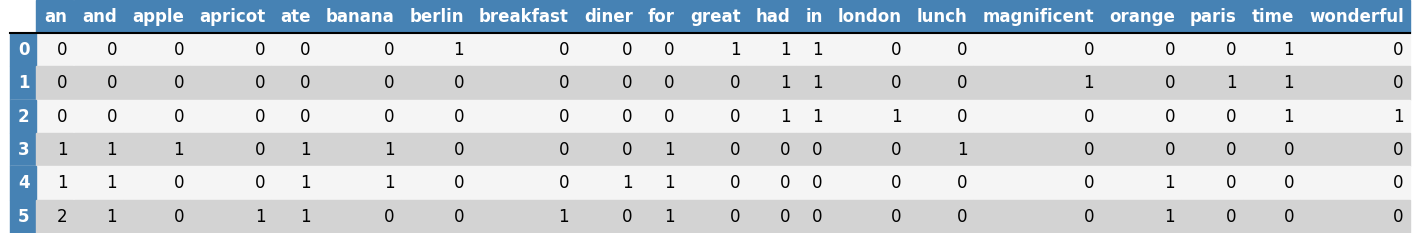
\includegraphics[width=1.0\textwidth]{Assets/topic_model_count_vector}
    \caption{Document Term Matrix}
    \label{fig:document_term_matrix}
\end{figure}

The \gls{document_term_matrix} is shown in Fig.\ref{fig:document_term_matrix} where the header row represents the \gls{vocabulary}.
The data entries in the table are the counts for each \gls{vocabulary} term in each \gls{document}.


\section{Traditional Methods}\label{sec:traditional-methods}

\subsection{One-Hot-Encoding}\label{subsec:one-hot-encoding}
Each \gls{document} in the Fig.\ref{fig:sample_docs} can be represented by the respective row in Fig.\ref{fig:document_term_matrix} when interpreted as a vector.
$$\vec{document_0} = [\;0\;0\;0\;0\;0\;0\;1\;0\;0\;0\;1\;1\;1\;0\;0\;0\;0\;0\;1\;0\;]$$
If such vectors only contain binary ones and zeros, i.e. if they do not count word occurrences but only indicate if a word is present or not, such vectors are called One-Hot encoded vectors.


\subsection{Bag-of-Words}\label{subsec:bag-of-words}
The \gls{document_term_matrix} shown in Fig.\ref{fig:document_term_matrix} also contains word counts as can be seen from the \gls{document} in the last row:
$$\vec{document_5} = [\;2\;1\;0\;1\;1\;0\;0\;1\;0\;1\;0\;0\;0\;0\;0\;0\;1\;0\;0\;0\;]$$
Such vectors are known as Bag-of-Word vectors as they account for the frequency of a word in a \gls{document}.

\subsection{Document Similarities}\label{subsec:document-similarities}
After vectorization, it is possible to calculate similarities between sentences mathematically.
One common way to do that is to calculate the cosine similarity of the desired vectors which is the cosine of the angles between the two vectors \cite{CosineSimilarity}:

\begin{equation}
cosine\;similarity\,{_{ab}} = \frac{\vec{a} \cdot  \vec{b}^{\;T}}{\lvert{\vec{a}}\rvert \cdot \lvert{\vec{b}}\rvert}\label{eq:cossim1}
\end{equation}

For instance: The cosine similarity between document 0 and document 1 of the Sample Documents (Fig.\ref{fig:sample_docs}) is calculated by:

$$ cosine\;similarity\,{_{01}} = \frac{\vec{document0} \cdot  \vec{document1}^{\,T}}{\lvert{\vec{document0}}\rvert \cdot \lvert{\vec{document1}}\rvert} = 0.60 $$

The high cosine similarity of 0.60 is also attributed to the fact that both documents contain the same words
$$ [\;I,\;had,\;a,\;time,\;in\;] $$
some of which are considered \gls{stop_words} that do not carry much semantic information.

\subsection{Feature Dimension Reduction}\label{subsec:techniques-to-reduce-vocabulary}
Usually a \gls{document} contains far fewer terms than a \gls{vocabulary} which results in sparse vectors where many features have zero values.
Sparse vectors not only increase the computational complexity and the risk to overfit a Machine Learning model, but also are a sign that some
important information in the data is missing \cite{ProblemsWithSparseVectors}.
For this reason, it is common practice to reduce the \gls{vocabulary} and so the vector and feature dimension.

\subsubsection{Remove Stop Words}\label{subsubsec:remove-stop-words}
\gls{stop_words} include articles, conjunctions, prepositions, pronouns and very common verbs such as \emph{is}.
They appear in most \glspl{document} and thus do not contribute to distinguish them.
Beside commonly known \gls{stop_words} in a \gls{corpus}, there might be additional domain-specific \gls{stop_words} such as the word for the currency unit \emph{Euro} in finance-related \glspl{document}.

\subsubsection{Remove Function Words}\label{subsubsec:remove-function-words}
\gls{nlp} differentiates between \gls{content_words} and \gls{function_words}.
\gls{function_words} help to construct the grammatical relationships in a sentence whereas \gls{content_words} serve to carry their semantic meaning.
In Topic Modelling, the target is to extract semantics. Thus, \gls{function_words} are less relevant and can be removed.

\subsubsection{Reduce words to their Lemmas and Stems}\label{subsubsec:word-lemmas}
Words appear in many different inflectional forms such as verb tenses (past, present and future) and pluralizations.
\gls{lemmatization} is the process to convert all such forms to the lemma or root of the word \cite{Lemmatization}.
This process removes some contextual information but usually well preserves the semantic meaning of the text.
\gls{stemming} reduces a word to its word stem by clipping off some suffix chars.
Contrary to \gls{lemmatization}, this process can change the semantic meaning of the word (for instance: \emph{fisher}\textrightarrow \emph{fish}) and thus must be
applied carefully.
Nevertheless, both methods drastically reduce the size of the \gls{vocabulary}.

\subsubsection{Others}\label{subsubsec:others}
Other methods to reduce the \gls{vocabulary} include the removal of non-words such as punctuation chars and numbers from the text.
If nouns in a specific domain carry proportionally more information than other words, it might be beneficial to remove all non-noun words.


\subsection{TF-IDF}\label{subsec:tf-idf}
It is known from Information Theory that low probability terms carry much more information than high probability terms \cite{EntropyInformationTheory}.
Low probability terms are those words that appear very seldom in a \gls{corpus} or in the \glspl{document} that were used to train commonly used \glspl{llm}.
If such low probability words appear much more frequently in a certain \gls{document} than in the related \gls{corpus}, this might be an indication
that this word is important to understand the context of the particular \gls{document}.
This is the concept of \gls{tfidf}:

\begin{gather}\label{eq:tfidf}
    \emph{TF-IDF} = TF * IDF
\notag \\ \notag \\
    \emph{TF} = \frac {\textrm{number of times the \textbf{term} appears in the document} }{ \textrm{total number of terms in the document}}
\notag \\ \notag \\
    \emph{IDF} = log\; (\frac {\textrm{number of documents in the corpus}} {\textrm{number of documents in the corpus containing the \textbf{term}}})
\notag \\ \notag \\
\end{gather}

The Term Frequency (TF) is the frequency a target word appears in a given \gls{document}.
In a Bag-of-Word approach (Sec.\ref{subsec:bag-of-words}), this number would go into the \gls{document_term_matrix}, but
in \gls{tfidf}, it is first multiplied by the Inverse Document Frequency (IDF).
The IDF is the logarithm of the number of all \glspl{document} divided by the number of those \glspl{document}
that contain the target word.
If the frequency of the target word in all \gls{document} is low, then the IDF will be high and this will increase the weight of
the target word in the \gls{document_term_matrix}.
This can be seen from the \gls{document_term_matrix} in Fig.\ref{fig:document_term_matrix_tfidf} when \gls{tfidf} vectorization was used:

\begin{figure}[H]
    \centering
    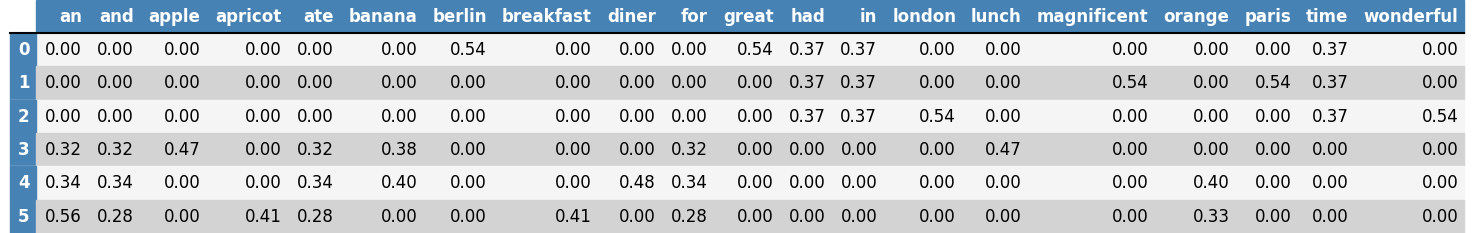
\includegraphics[width=1.0\textwidth]{Assets/topic_model_tfidf_vector}
    \caption{Document Term Matrix with TF-IDF}
    \label{fig:document_term_matrix_tfidf}
\end{figure}

Words that appear only once in all \glspl{document} (for instance the word \emph{apple}) have a higher weight in the \gls{tfidf} \gls{document_term_matrix} than words
that appear very often (for instance the word \emph{ate}).

%%%%%%%%%%%%%%%%%%%%%%%%%%%%%%%%%%%%%%%%%%%%%%%%%%%% EMBEDDINGS
\section{Word Embeddings\protect\footnote{This section was mainly taken from \cite{LfdTalk15}}}\label{sec:word-embeddings}


\subsection{Static Word Vectors}\label{subsec:static-word-vectors}

As explained in section \ref{subsec:one-hot-encoding}, words can be represented as one-hot encodings as also shown in the example in Fig.\ref{fig:onehot}.

\begin{figure}[H]
	\centering
	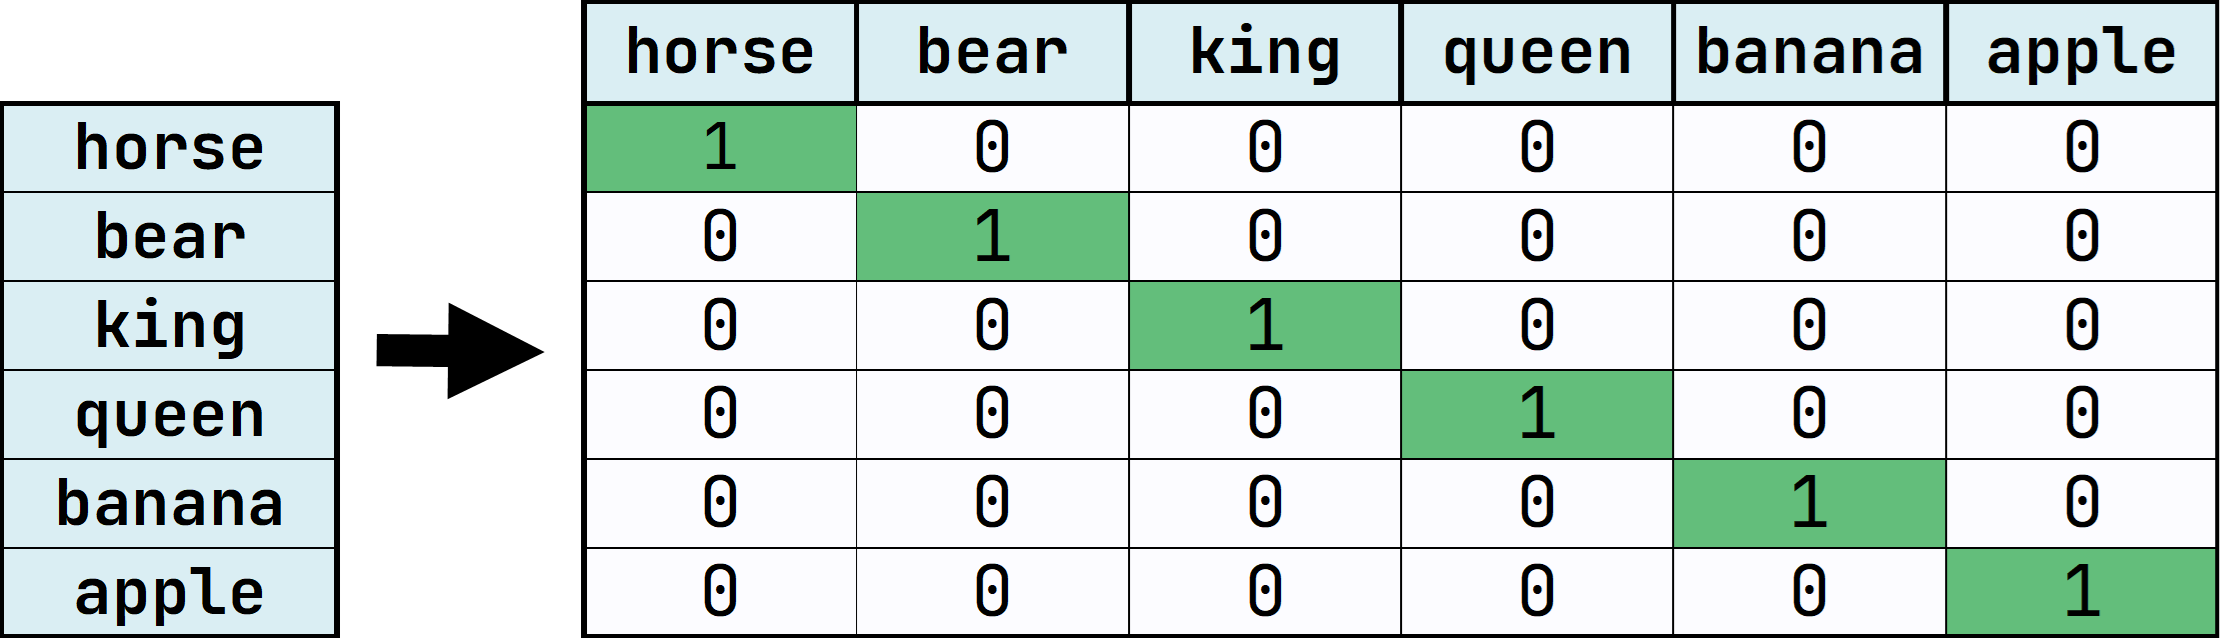
\includegraphics[width=0.7\textwidth]{Assets/onehot}
	\caption{One-Hot example}
	\label{fig:onehot}
\end{figure}

The first disadvantage of this approach is the computational inefficiency as each word in our simple example in Fig.\ref{fig:onehot} would require a sparse six-column vector with five 0's and only one 1.
The second disadvantage is that this approach does not encode syntactical or semantic word similarities as similar words would have different and unrelated vector representations.

\subsubsection{Manually crafted features}
To encode syntactical or semantic word commonalities, one could think about word characteristics or attributes and manually encode the magnitude of those attributes for each word as shown in Fig.\ref{fig:wordfeaturesmanually}.
A \emph{horse} is an \emph{animal}, one \emph{can ride it}, it has \emph{four legs} and is usually \emph{peaceful}.\\
This is very similar to the \gls{vocabulary} in the \gls{tfidf} and \emph{Bag-of-Word} approach outlined in Section \ref{subsec:tf-idf}, but differes from
it in that the features here do not represent actual words but contextual concepts.
The feature \emph{animal} only has values in its respective vector position, not when the \emph{word} \emph{animal} itself appears, but only when the \emph{contextual concept} of an \emph{animal} appears.

\begin{figure}[H]
	\centering
	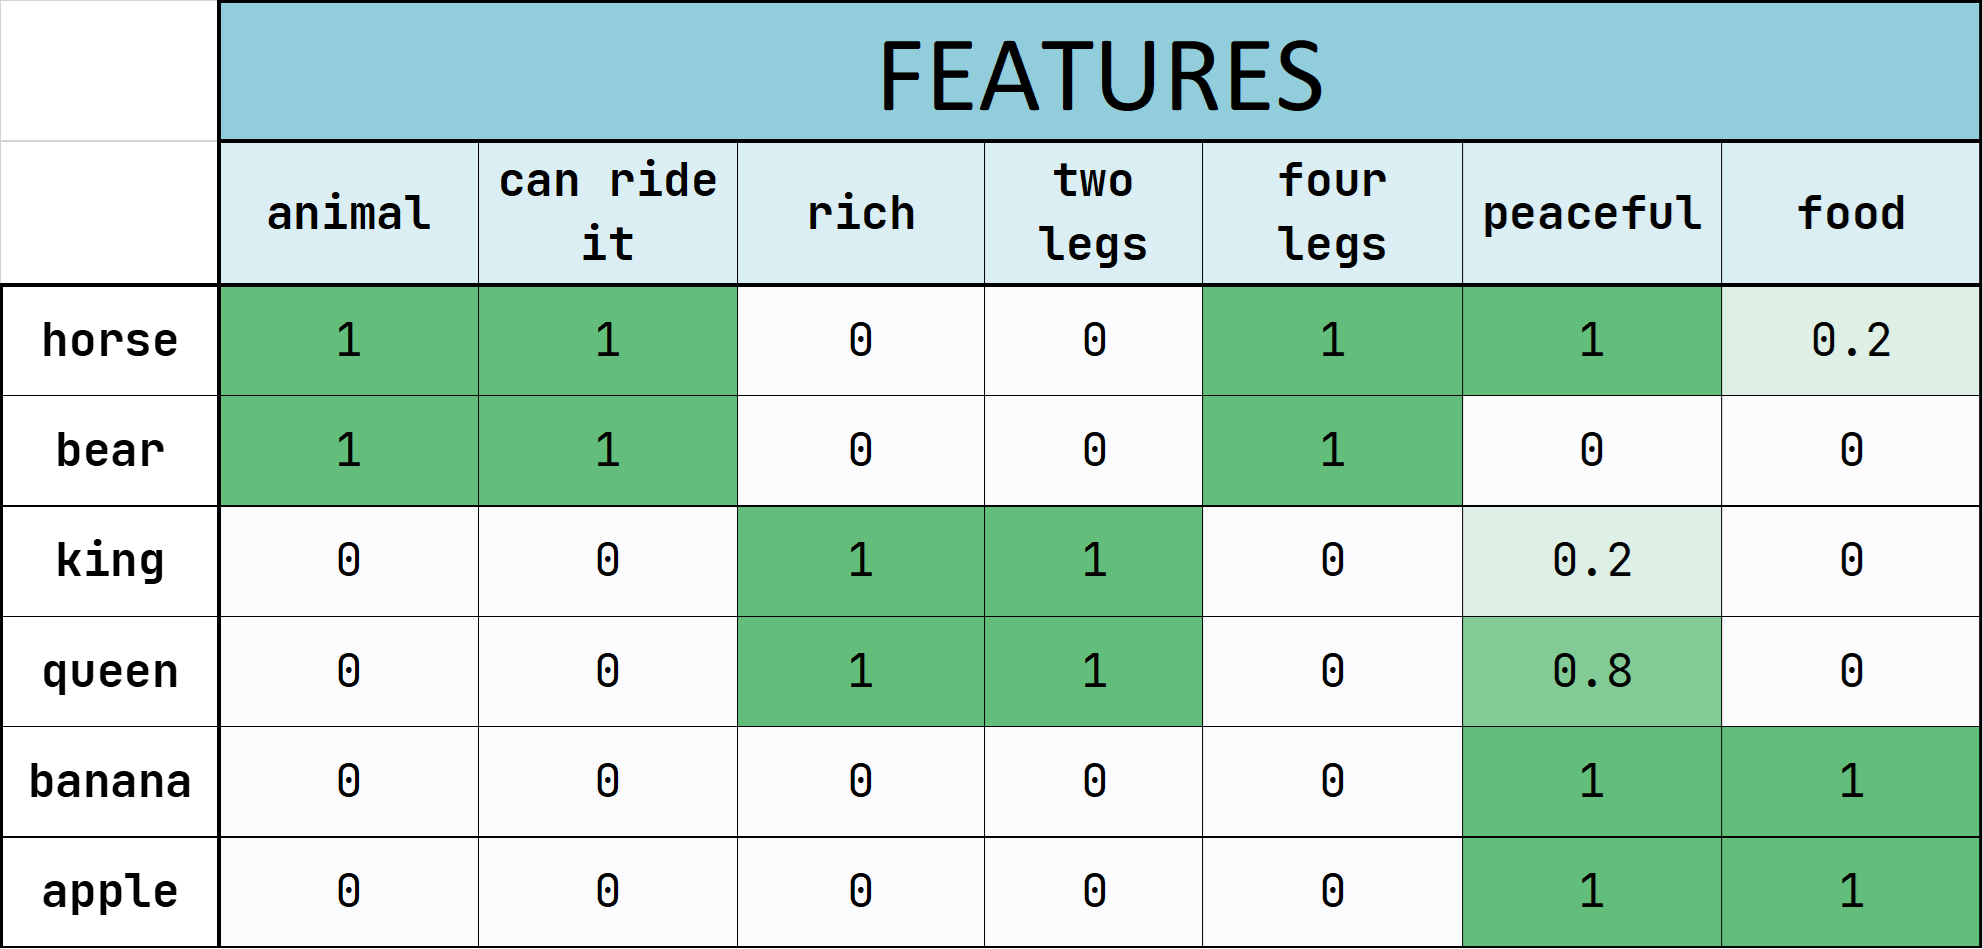
\includegraphics[width=0.7\textwidth]{Assets/wordfeaturesmanually}
	\caption{Manually Crafted Features}
	\label{fig:wordfeaturesmanually}
\end{figure}

The word \emph{horse} would then be represented as a vector of values for each of these handcrafted features (Fig.\ref{fig:horsevector}):

\begin{figure}[H]
	\centering
	
\includegraphics[width=0.7\textwidth]{Assets/horsevector}
	\caption{Word vector for the word \emph{horse}}
	\label{fig:horsevector}
\end{figure}

This approach ensures that related words are represented similarly as their values in the respective vector position are close to each other.
Such similarities can also be calculated numerically by applying the cosine similarity method, see Equation \ref{eq:cossim1}.
The cosine similarities between each pair of words in Figure \ref{fig:wordfeaturesmanually} are depicted in Fig.\ref{fig:cossimvalues}.

\begin{figure}[H]
	\centering
	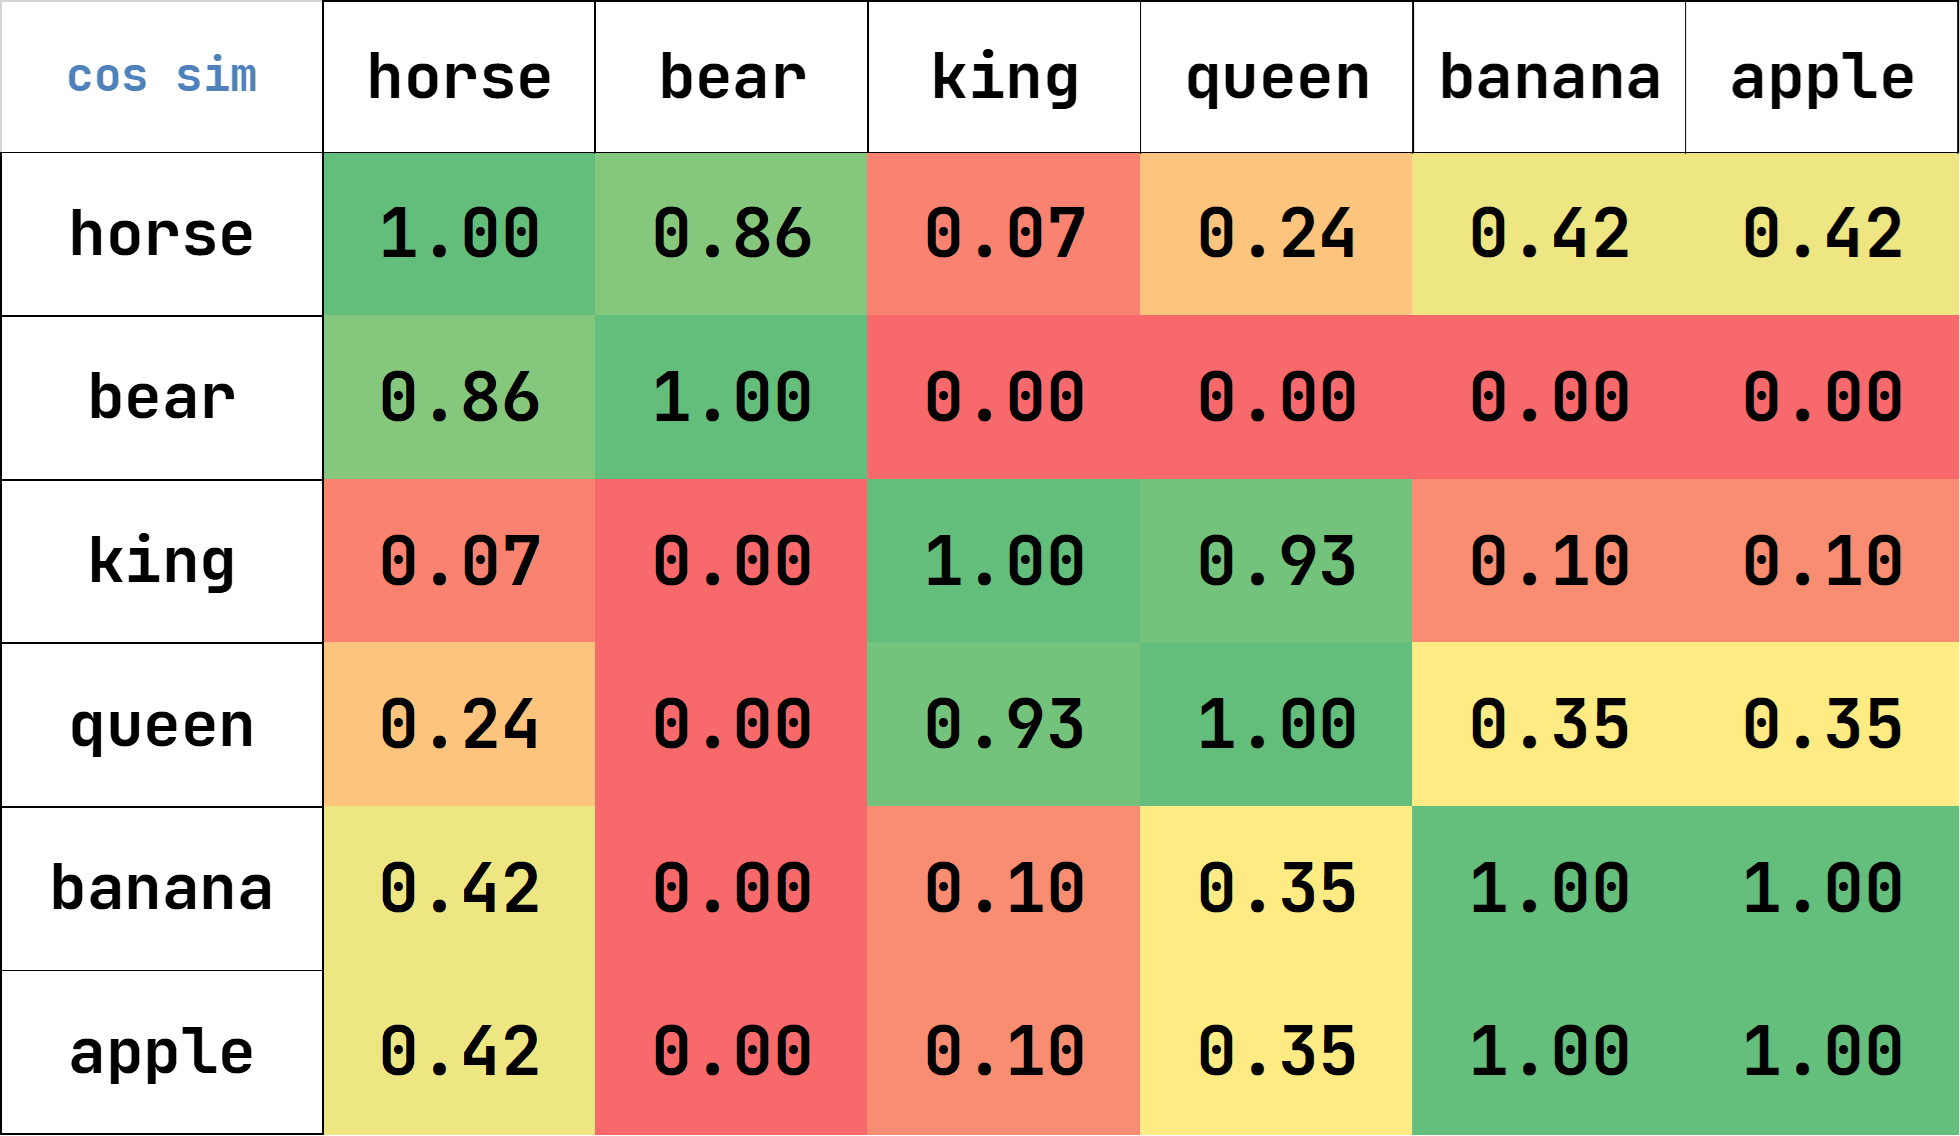
\includegraphics[width=0.6\textwidth]{Assets/cossimvalues}
	\caption{Exemplary Cosine Similarity Matrix based on Fig.\ref{fig:wordfeaturesmanually}.}
	\label{fig:cossimvalues}
\end{figure}

The cosine similarity for the word pair \emph{horse} and \emph{apple}, for instance, yields a value of 0.42.
For the word pair \emph{apple} and \emph{banana} however, this value is 1.0, owing to the fact that both are fruits and in our simple example have the same feature values at each index position of their word vector.

\subsubsection{Learned features}
Manually crafting feature values for every word in a vocabulary is cumbersome at best.
Better than crafting features by hand is to have a machine learning model to learn these features and feature values.
This is the \emph{word2vec} approach Mikolov et al. proposed in their seminal papers in 2013 \cite{word2vec1,word2vec2}.
A shallow, two-layer \gls{ann} (Fig.\ref{fig:featureslearned}) is trained with sentences that contain a masked word to be predicted (target or dependent variable) based on its non-masked adjacent words (input or independent variables) in that sentence.

\begin{figure}[H]
	\centering
	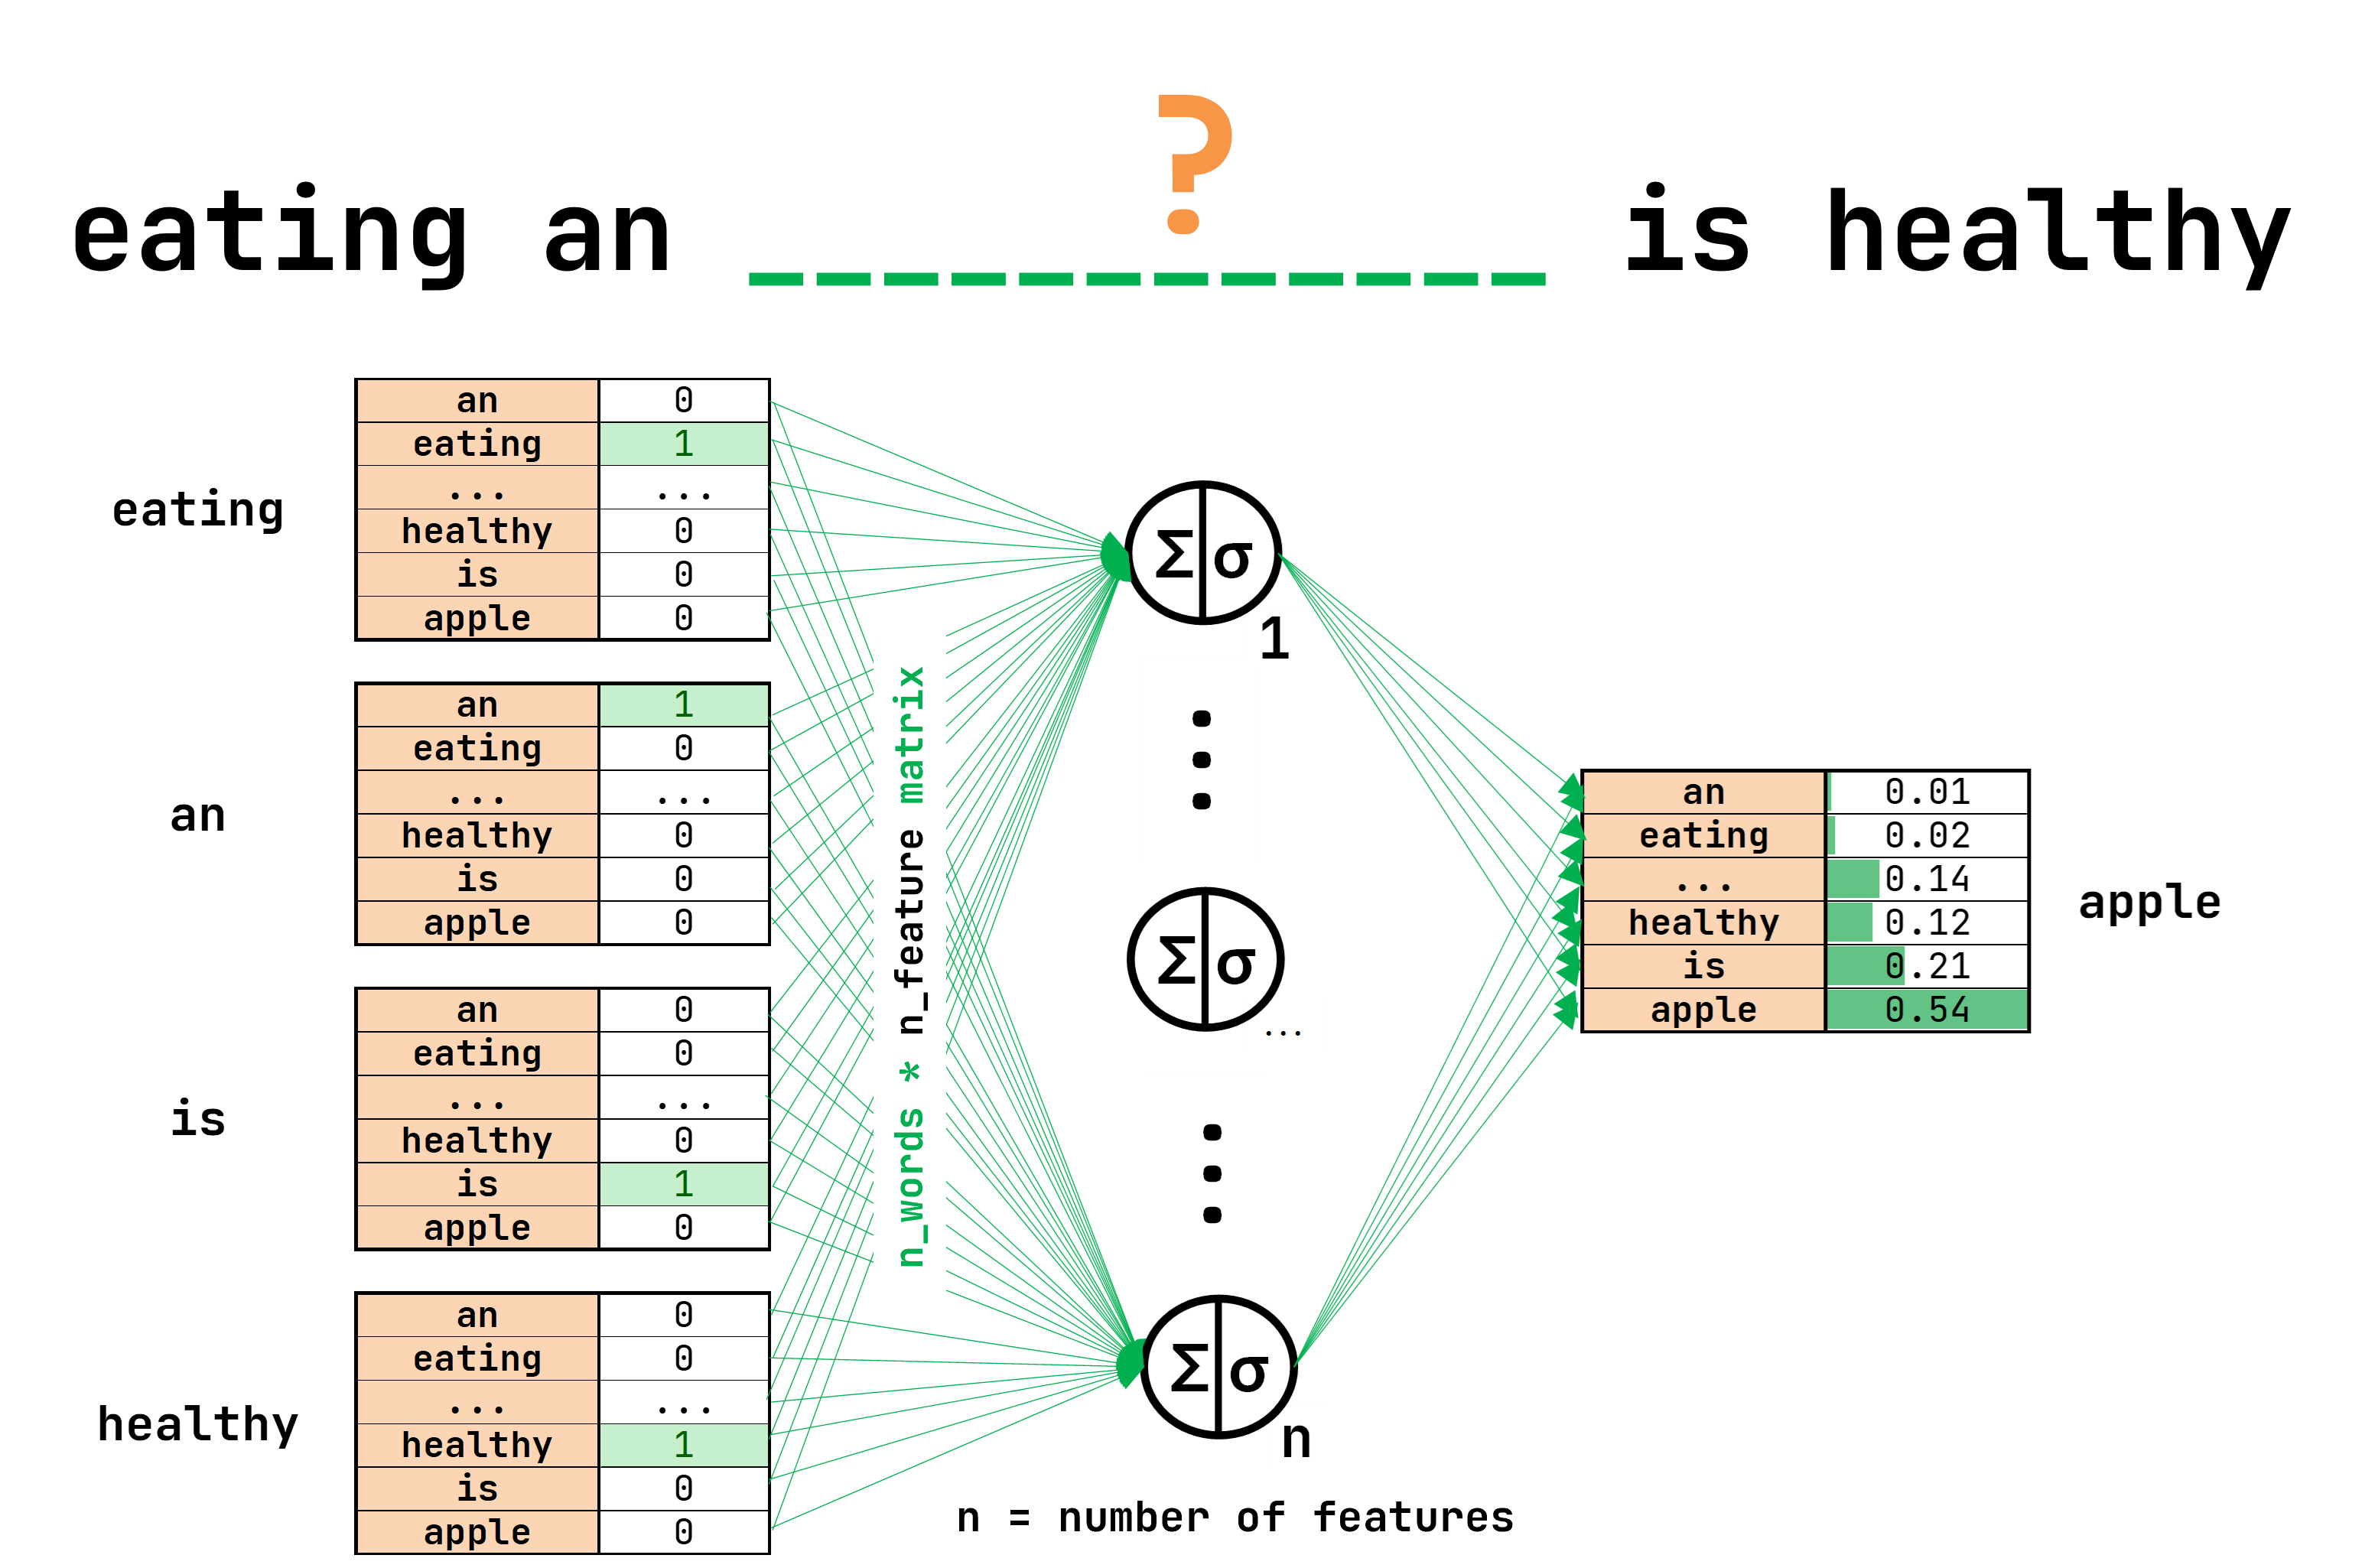
\includegraphics[width=0.6\textwidth]{Assets/featureslearned}
	\caption{word2vec: Masked words learned by a shallow, two-layer \gls{ann}.}
	\label{fig:featureslearned}
\end{figure}

The number of learned features depends on the number of neurons in the middle layer and the learned weights represent the respective feature values.
The learned features do not have names as before (like \emph{animal}, \emph{rich}, \emph{food}, etc.) and thus cannot be interpreted semantically by humans (easily) (Fig.\ref{fig:featvalueslearned}).

\begin{figure}[H]
	\centering
	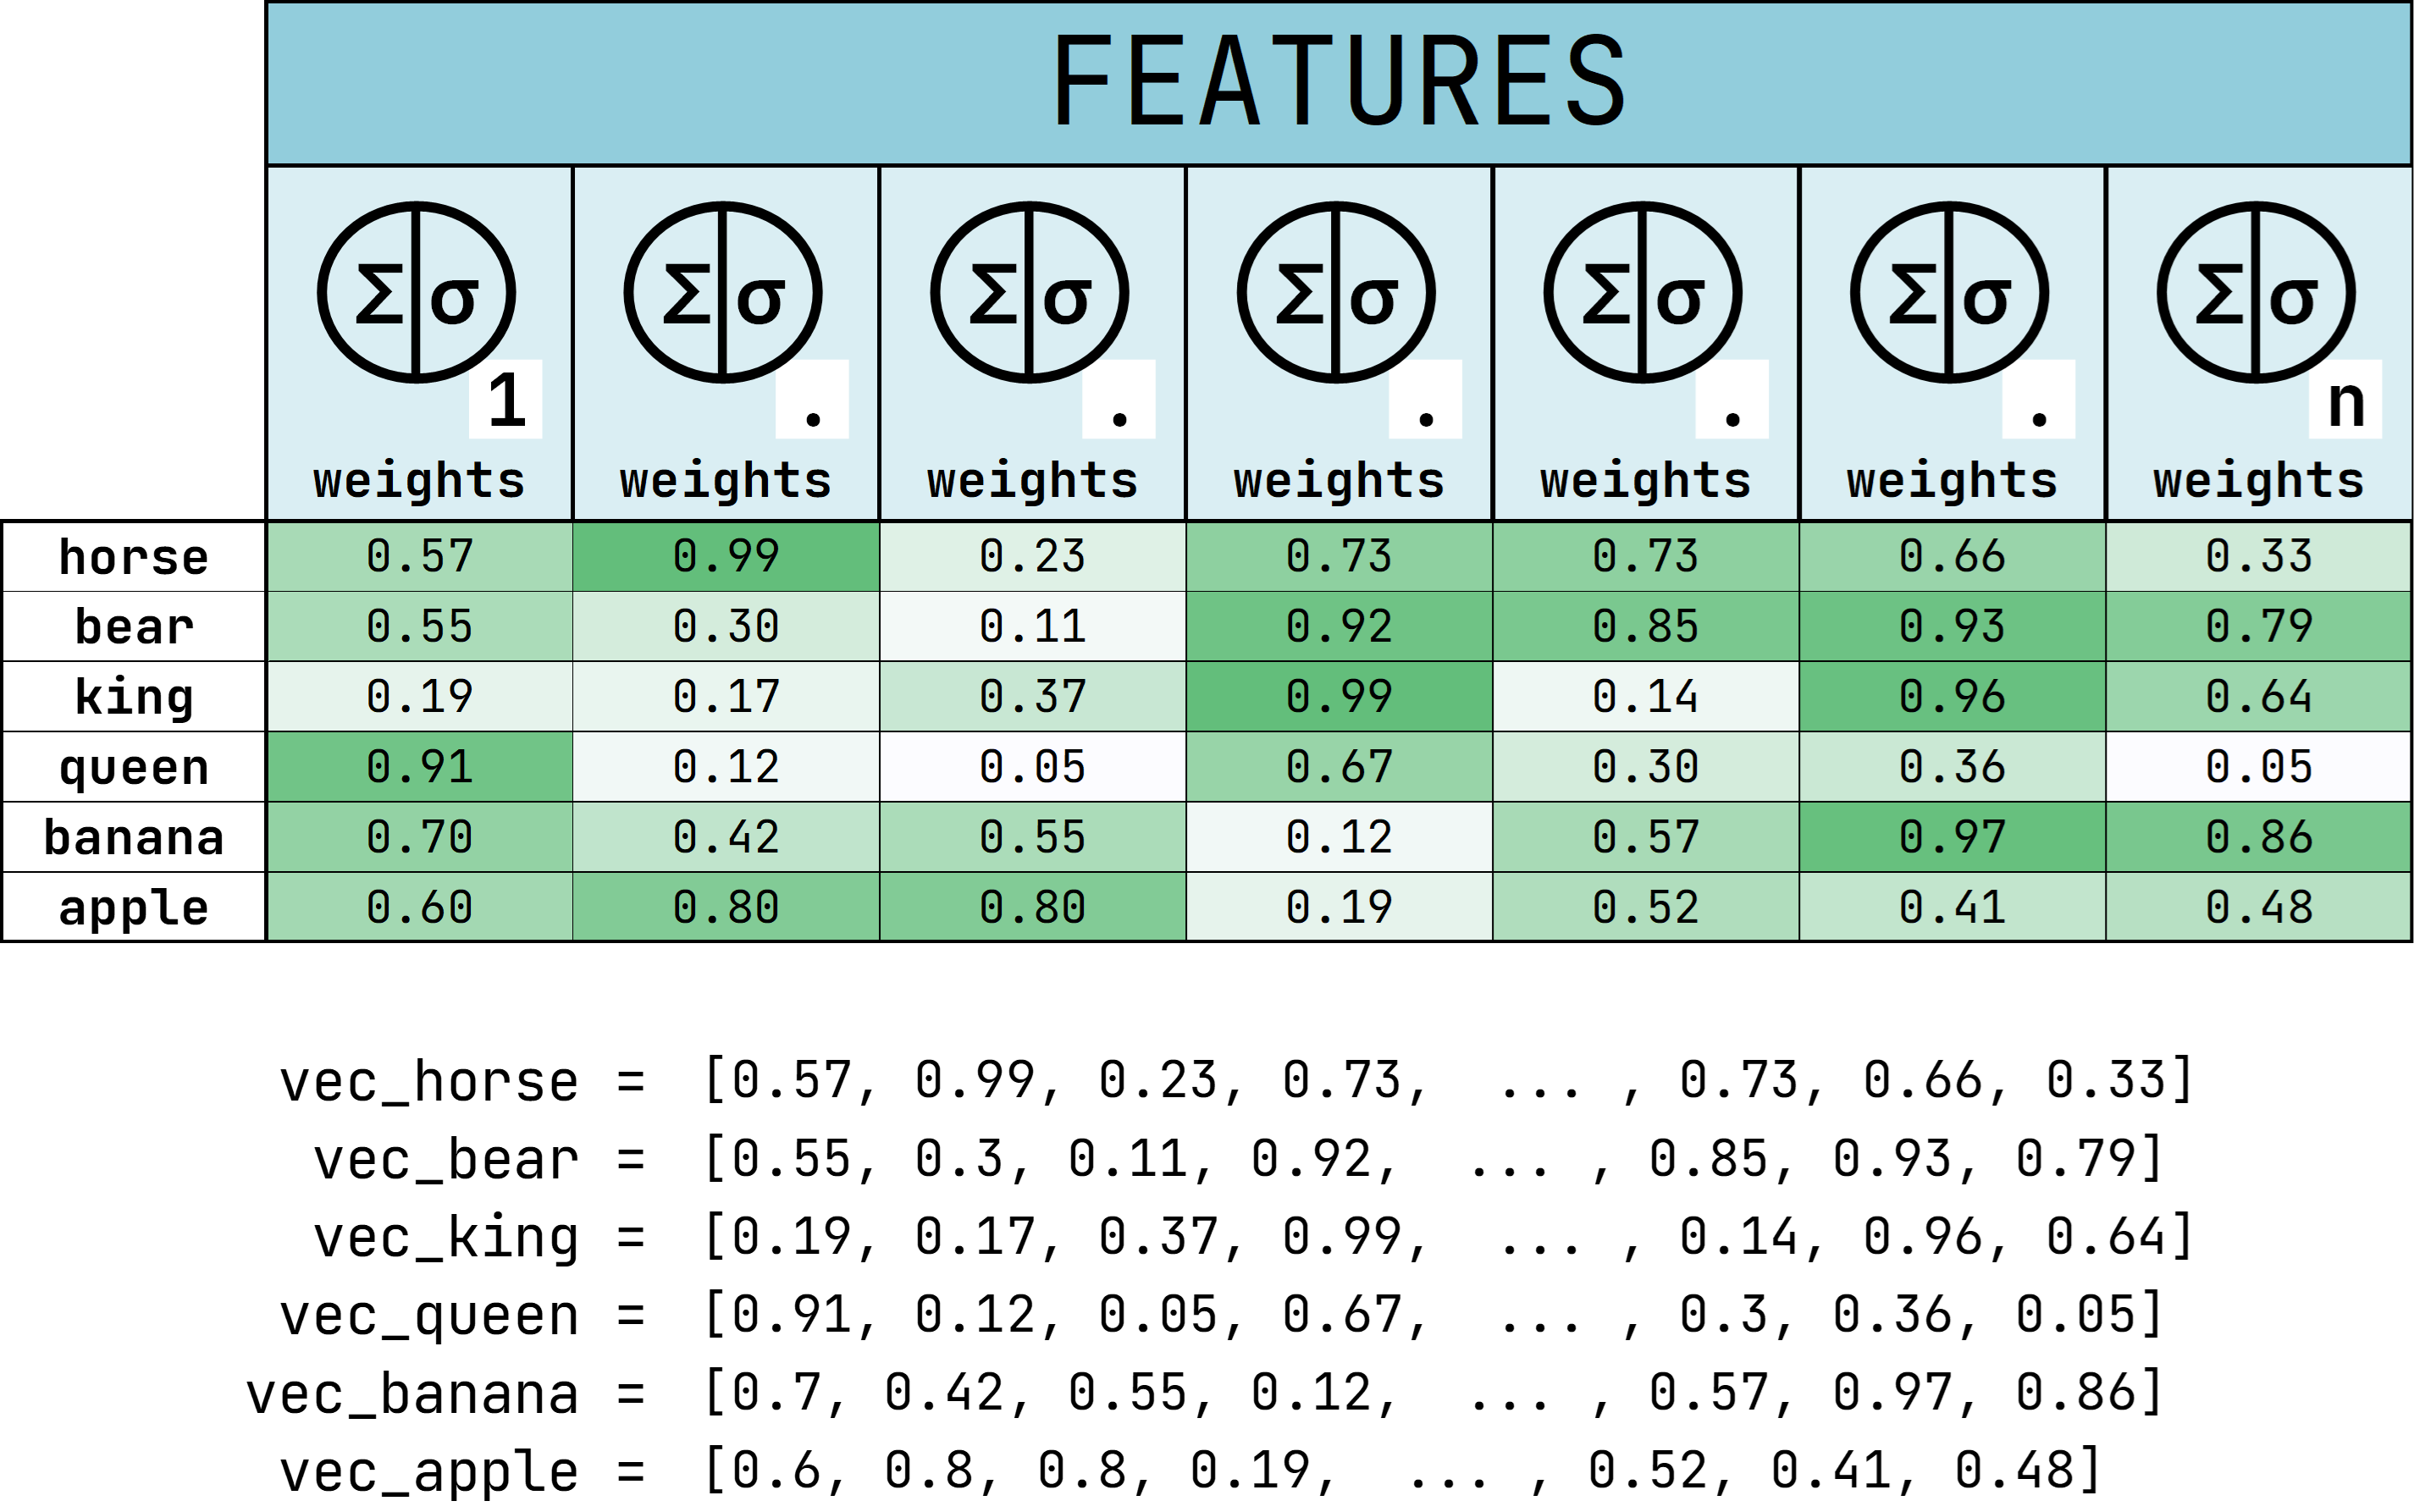
\includegraphics[width=0.8\textwidth]{Assets/featvalueslearned}
	\caption{The learned parameters/weights represent the feature values.}
	\label{fig:featvalueslearned}
\end{figure}

\subsubsection{The problem with static word embeddings}
The learned word vectors are also known as word embeddings and work well for tasks such as measuring similarities between individual words.
But they often fail when the scope goes beyond just words towards the semantic meaning of whole sentences.
A sentence is simply not just a chain of individual and independent words, but a construct containing interdependencies.

One of these word-wise interdependencies are homophones, i.e. words that are spelt the same but have different meanings.
The meaning of the word \emph{bank} in the sentence \emph{he withdraws money from his bank} is strongly affected by the surrounding words \emph{withdraws} and \emph{money} as they clearly suggest that \emph{bank} in that sentence refers to a financial institution.
In contrast, the meaning of the same word \emph{bank} in the sentence \emph{he was fishing in the river from a sand bank} is strongly affected by the words \emph{river} and \emph{sand} (Fig.\ref{fig:interdepend}).

\begin{figure}[H]
	\centering
	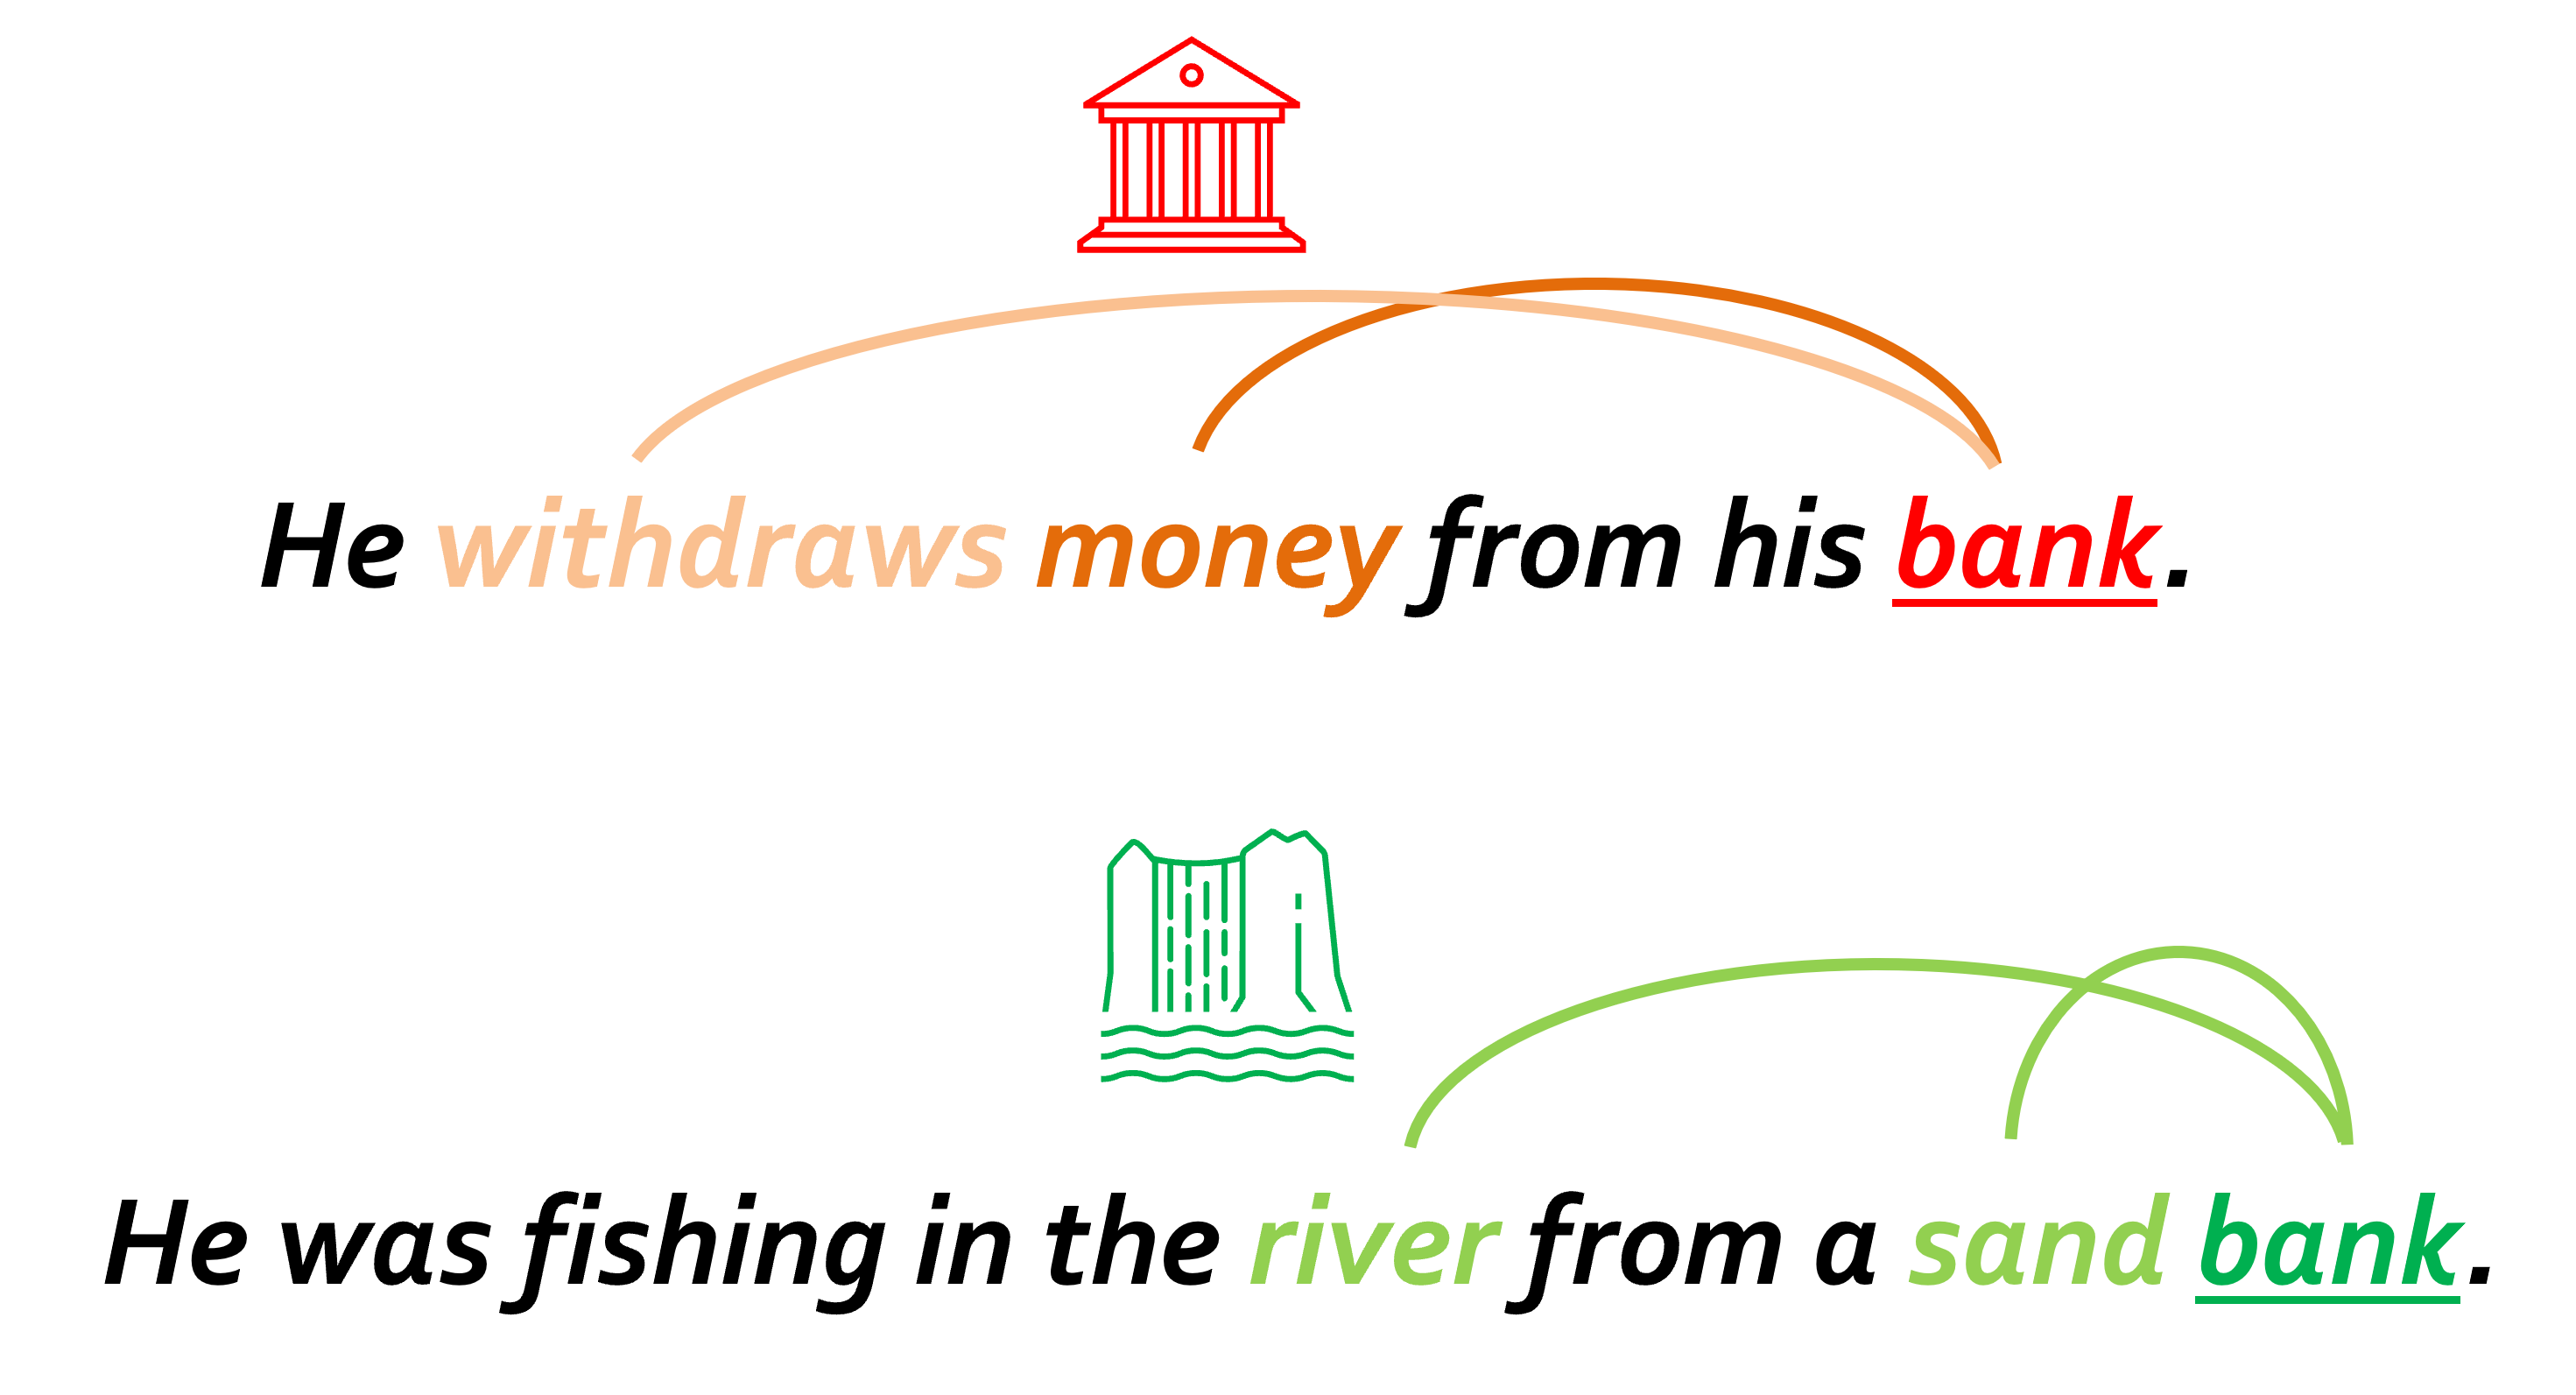
\includegraphics[width=0.7\textwidth]{Assets/interdepend}
	\caption{Homophone \emph{bank} dependent on its context}
	\label{fig:interdepend}
\end{figure}

When humans read these sentences, they derive the meaning of the word \emph{bank} by paying \emph{attention} to these adjacent words \cite{humanattention}.

There are more interdependencies in sentences than homophones, but in general it can be said that the meaning of a word depends on its respective context.
Word embeddings such as word2vec \cite{word2vec1,word2vec2} are static in the sense that they treat equal words alike without taking their context into account.
This is one of the reasons why static word embeddings such as word2vec often fail to understand the meaning of sentences.

\subsection{Contextual Word Embeddings}\label{subsec:contextual-word-embeddings}
It can surely be said, that in 2017 a single research paper changed the world: \emph{Attention is all you need} by Vasvani et al. \cite{aiayn} laid out a new \gls{ann}-architecture dubbed \gls{Transformer} that is able to embedd text contextually.
Transformers embrace the human \emph{attention} principle discussed above, i.e. the ability to infer the meaning of a word by paying \emph{attention} to its adjacent words in that sentence.

\subsubsection{Transformer Architecture}
The \gls{Transformer} architecture consists of \emph{Encoder} (left blocks in Fig.\ref{fig:transformers}) and \emph{Decoder} (right blocks in Fig.\ref{fig:transformers}) stacks.
The Encoder and Decoder stacks each have \emph{N} layers depending on the model version and size.
In the basic pre-trained \gls{BERT} \cite{BERT} model (\emph{bert-base-uncased}), which was one of the first models to implement the \gls{Transformer} architecture, \emph{N} is equal to 12, i.e. has 12 layers.

\begin{figure}[H]
	\centering
	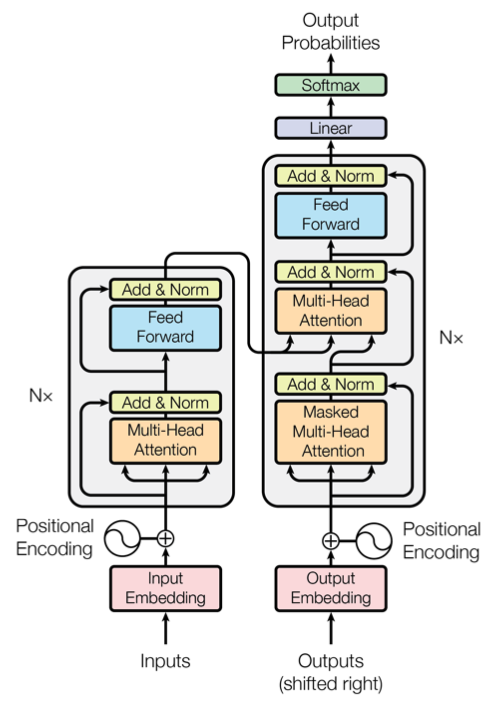
\includegraphics[width=0.4\textwidth]{Assets/transformers}
	\caption{\gls{Transformer} Architecture: Encoder and Decoder}
	\label{fig:transformers}
\end{figure}

For encoding text, only the Encoder part of the \gls{Transformer} is needed.
For generating text, the Decoder part is also needed (Fig.\ref{fig:transformers}).

\subsubsection{Self-Attention}
The central element in the architecture of \glspl{Transformer} is the \emph{self-attention mechanism} in the Multi-Head-Attention module depicted in Fig.\ref{fig:attn1}.

\begin{figure}[H]
	\centering
	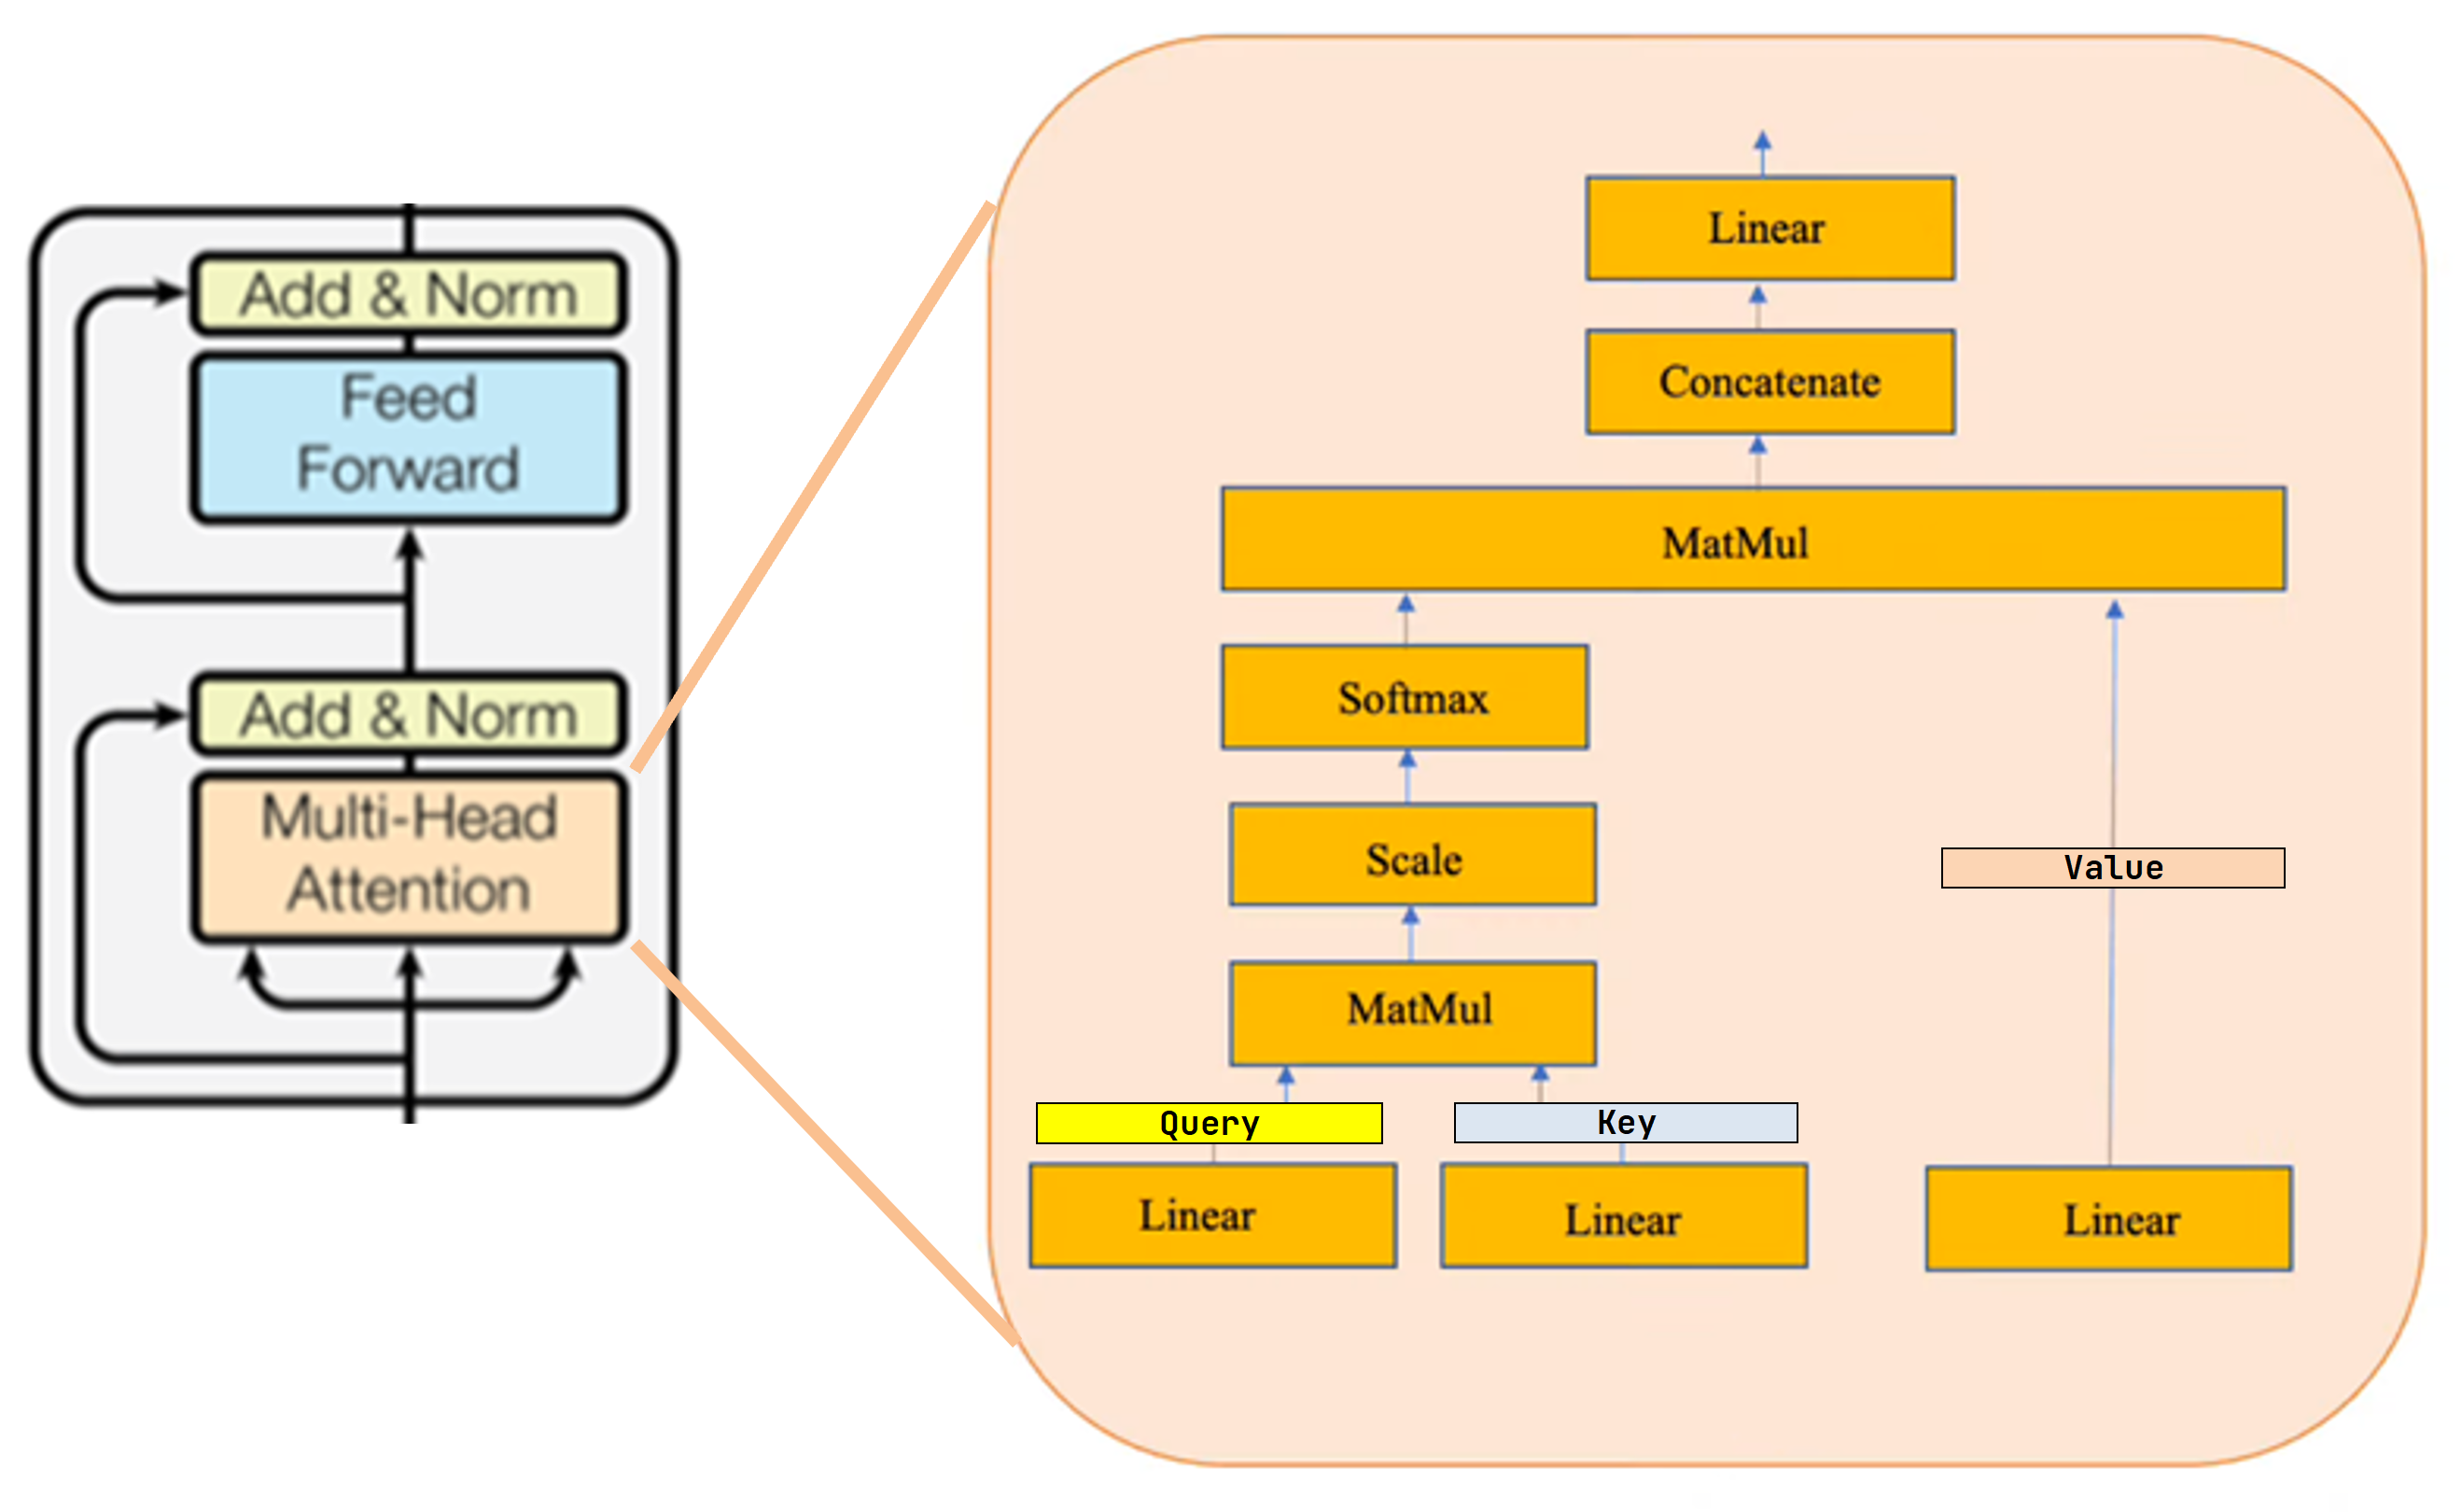
\includegraphics[width=0.7\textwidth]{Assets/attn1}
	\caption{Multi-Head Attention. Image from: \cite{BERT} and \cite{transformersyoutube}}
	\label{fig:attn1}
\end{figure}

In the Multi-Head-Attention module, three different matrices named \colorbox{yellow}{\emph{Query}}, \colorbox{cyan}{\emph{Key}} and \colorbox{orange}{\emph{Value}} are learned in the training phase based on one and the same static embeddings of the input words (Fig.\ref{fig:qkv1}).

\begin{figure}[H]
	\centering
	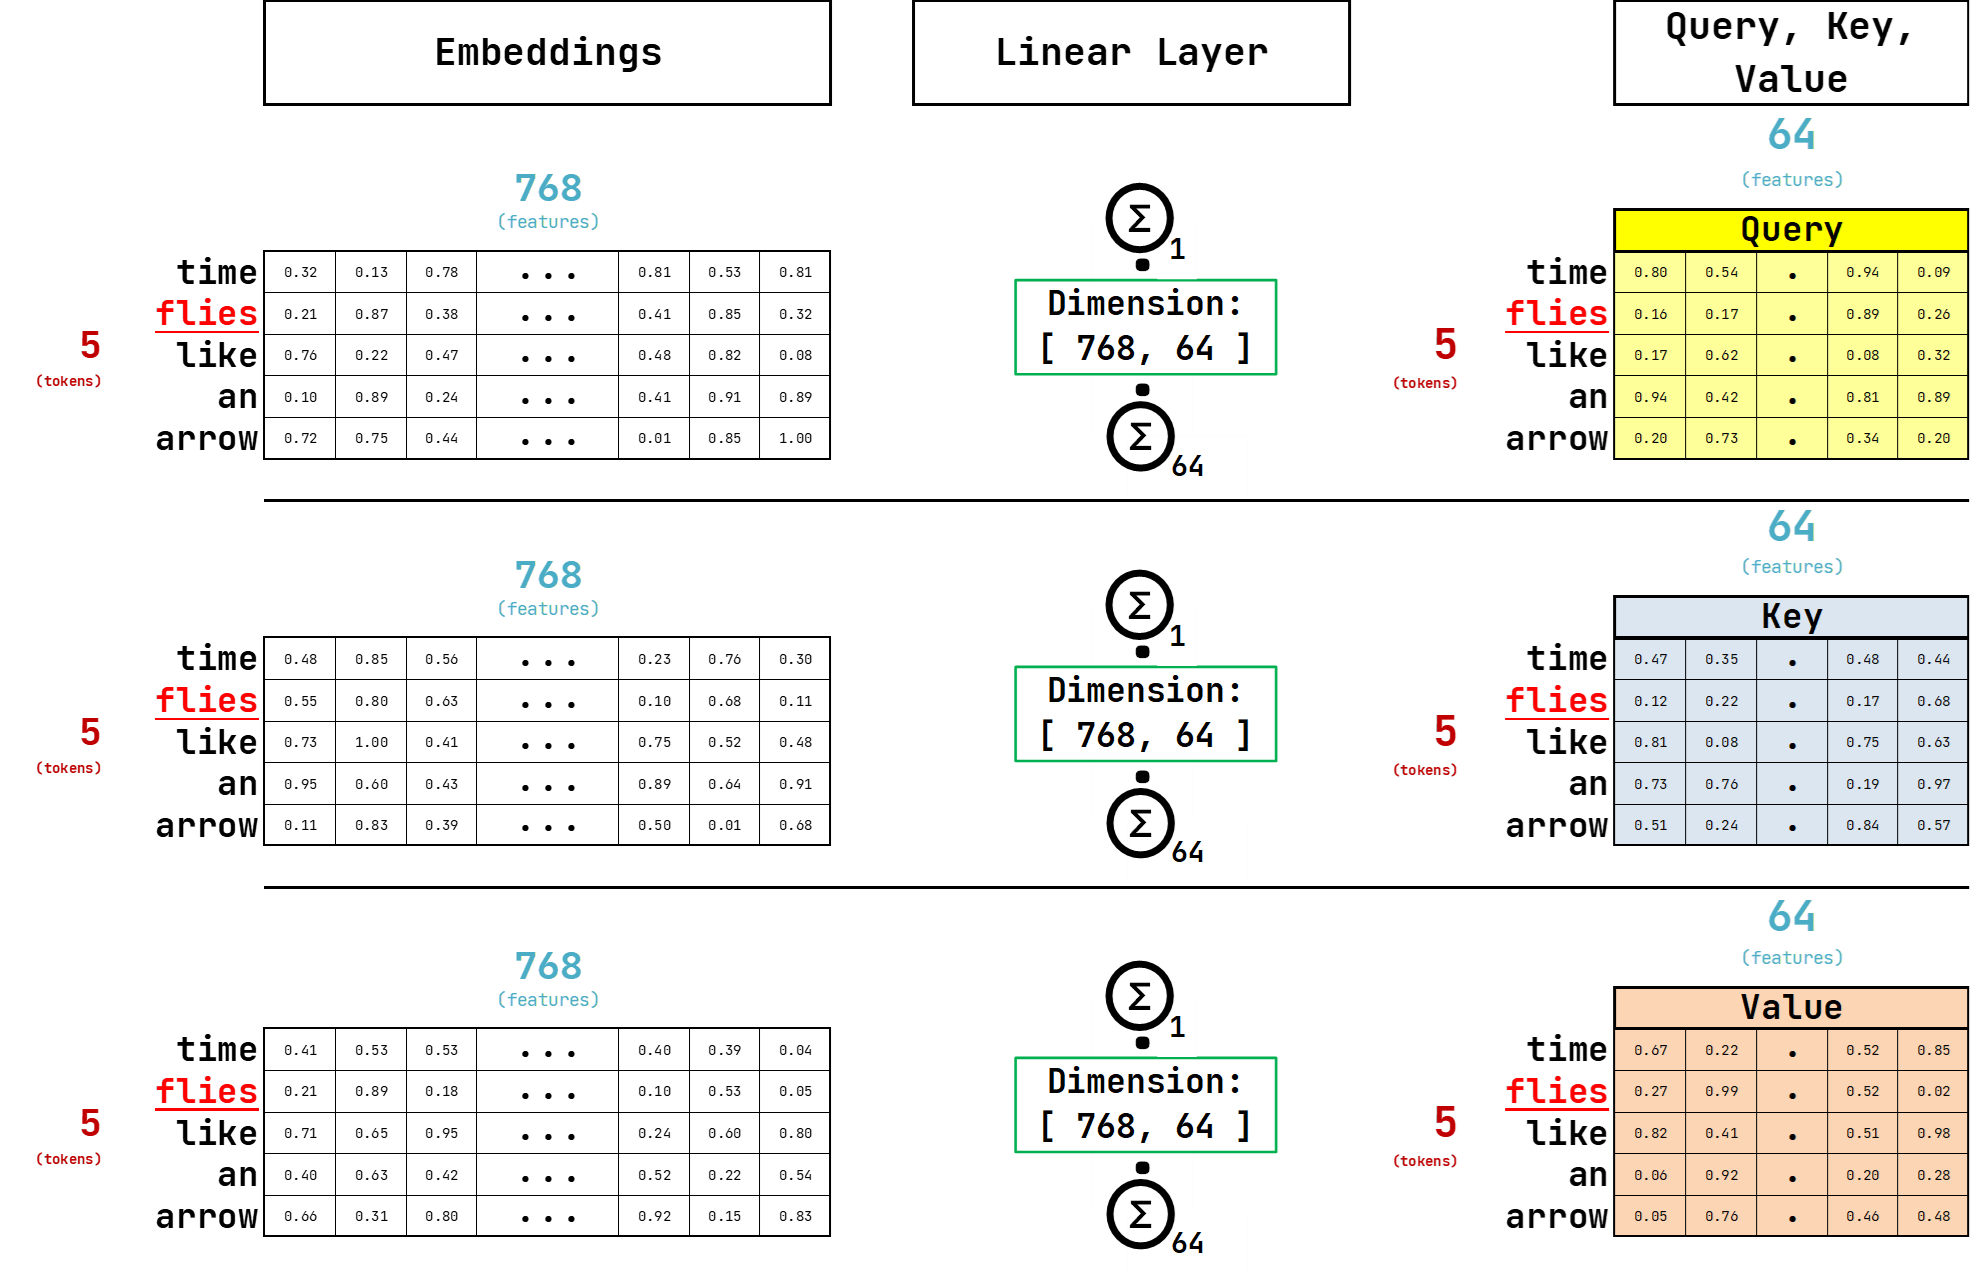
\includegraphics[width=0.7\textwidth]{Assets/qkv1}
	\caption{$Input Embeddings \cdot Linear Layer$ = \colorbox{yellow}{\emph{Query}}, \colorbox{cyan}{\emph{Key}}, \colorbox{orange}{\emph{Value}}}
	\label{fig:qkv1}
\end{figure}

The next step in the \emph{Multi-Head Attention} module during both, training and inference (in a downstream task), is the matrix multiplication depicted in Fig.\ref{fig:attnfilter} to produce the \colorbox{lime}{\emph{Attention Filter}}.
It has the same dimension ([5, 5] for the given sentence) as the length of the input text.
\begin{figure}[H]
	\centering
	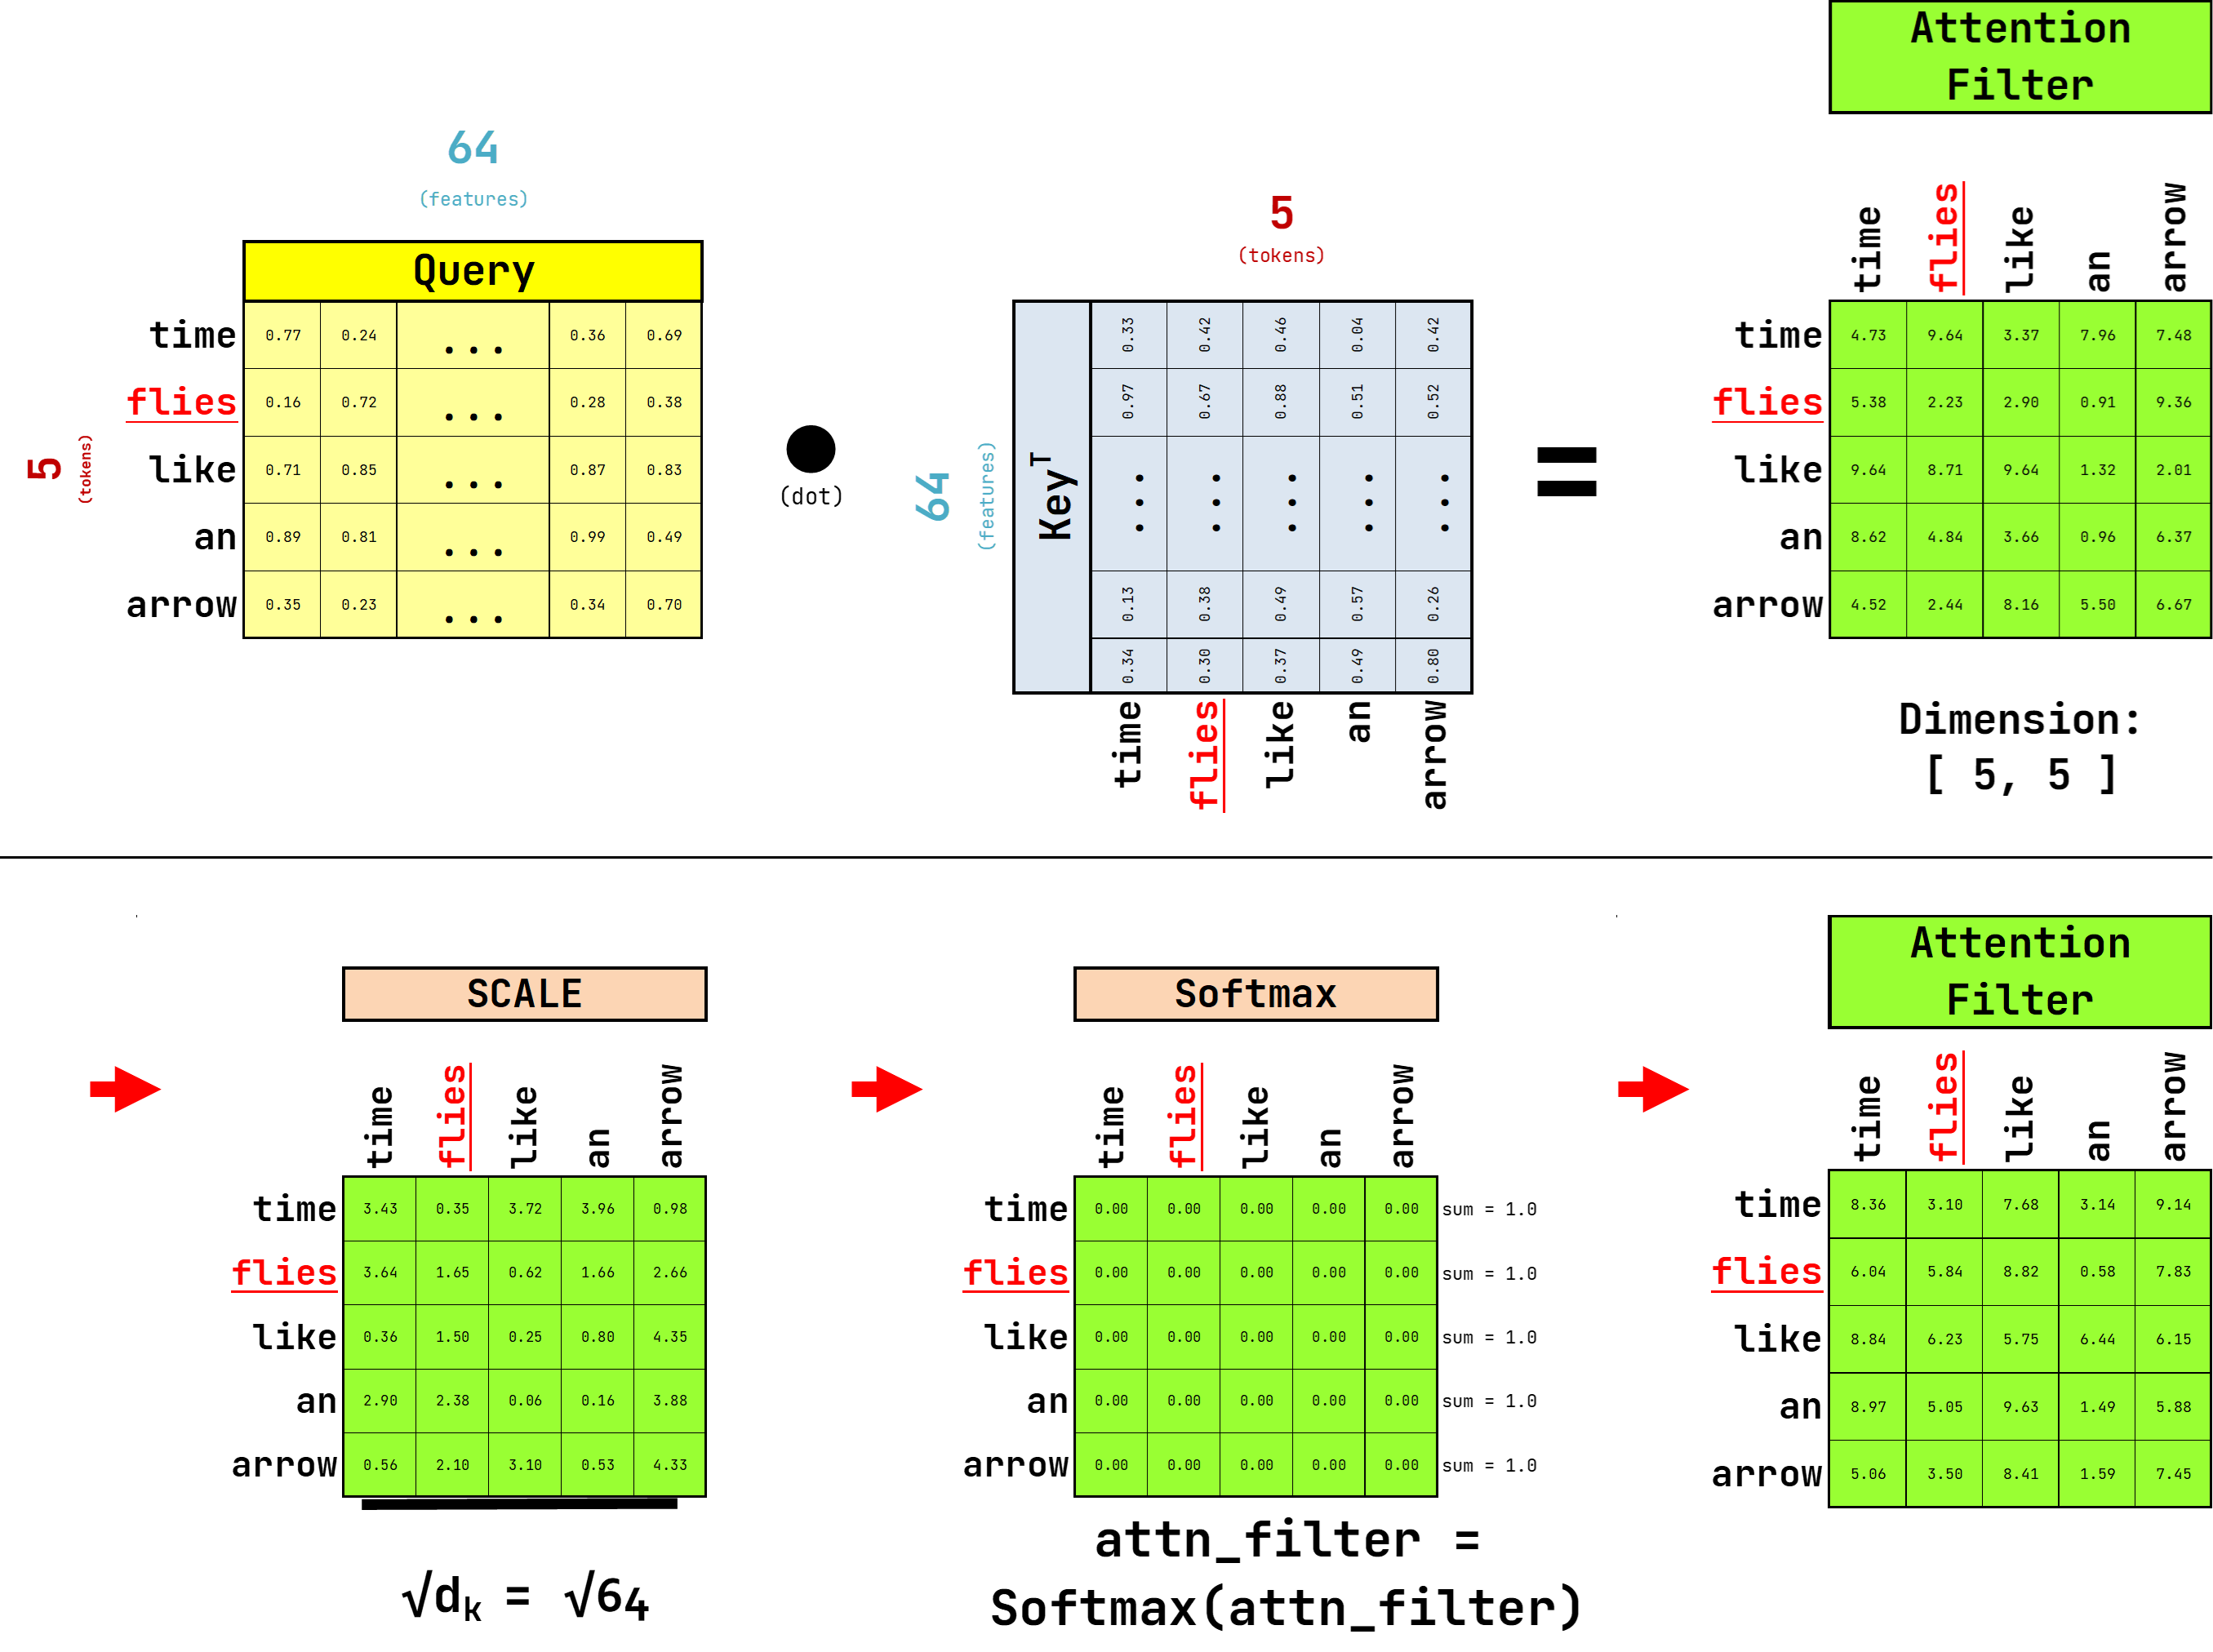
\includegraphics[width=0.7\textwidth]{Assets/attnfilter}
	\caption{$\colorbox{yellow}{\emph{Query}} \cdot \colorbox{cyan}{\emph{Key}}$ = \colorbox{lime}{\emph{Attention Filter}}}
	\label{fig:attnfilter}
\end{figure}

The task of the \colorbox{lime}{\emph{Attention Filter}} is to identify those adjacent words in a sentence that help determine the context for and
the meaning of a given word.

In the sample sentence \emph{time flies like an arrow}, a human reader would probably pay attention to the words \emph{arrow} and \emph{time} to determine the context and the meaning of the word \emph{flies}.
A well-trained \colorbox{lime}{\emph{Attention Filter}} would thus probably have higher values at the coordinate crossing for the word \emph{flies} (2nd row), \emph{time} (1st column) and \emph{arrow} (5th column).

The next step in the calculation process during training and inference is the most important and the main reason why \glspl{Transformer} can embedd context:
The multiplication of the \colorbox{lime}{\emph{Attention Filter}} with the \colorbox{orange}{\emph{Value}} matrix.

\begin{figure}[H]
	\centering
	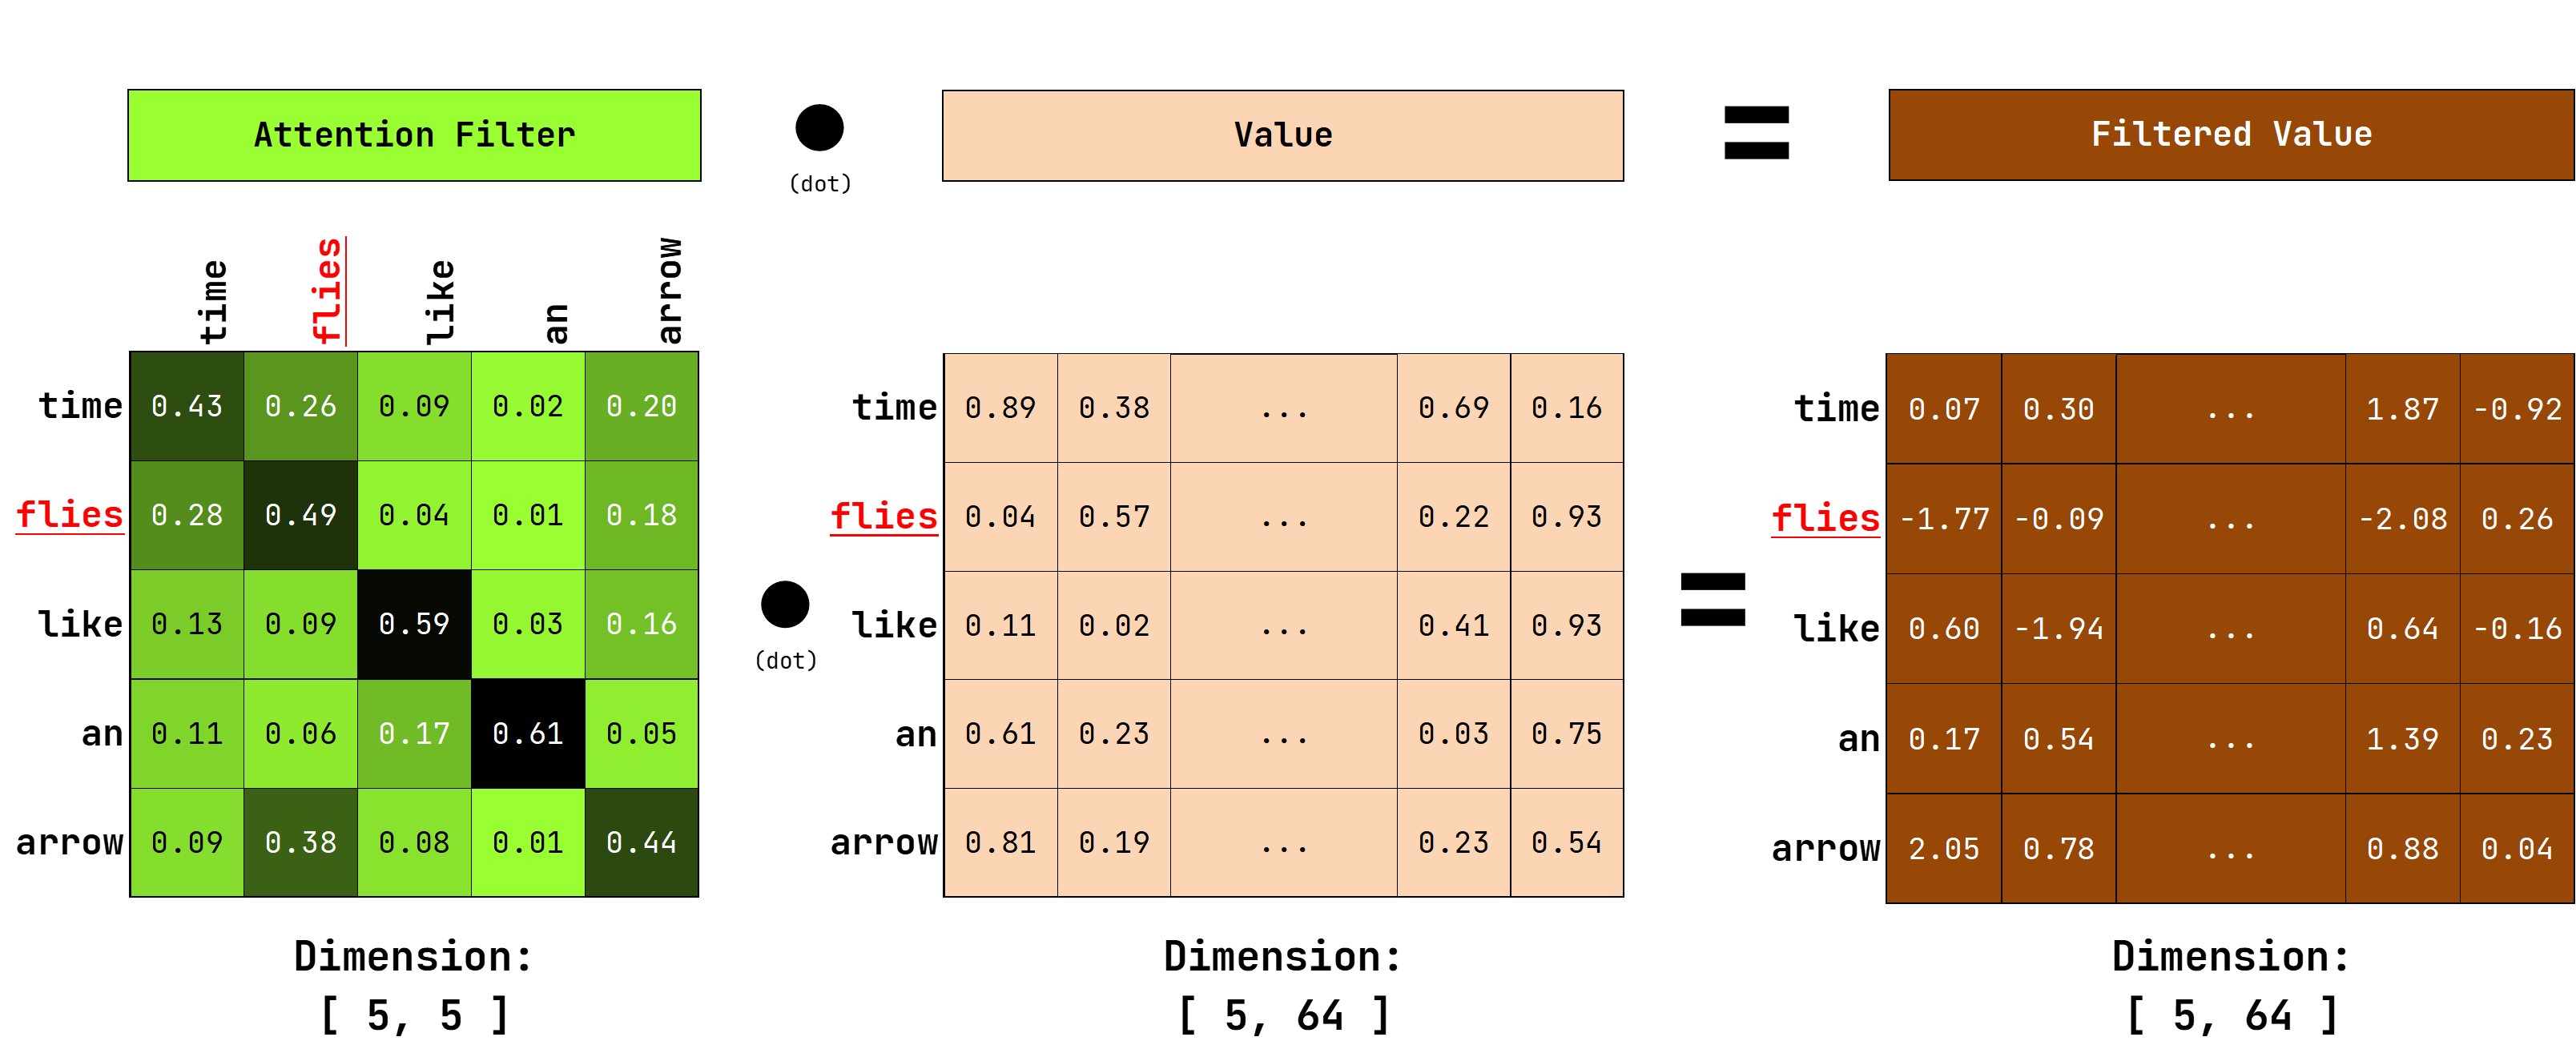
\includegraphics[width=0.7\textwidth]{Assets/filter1}
	\caption{$\colorbox{lime}{\emph{Attention Filter}} \cdot \colorbox{orange}{\emph{Value}}$ = \colorbox{brown}{\emph{Filtered Value}}}
	\label{filter1}
\end{figure}

The \colorbox{orange}{\emph{Value}} matrix is assumed to contain encoded information about the syntax and semantics of the input text though still static at this stage.
The \colorbox{lime}{\emph{Attention Filter}} multiplies the \colorbox{orange}{\emph{Value}} matrix carrying over those values to the \colorbox{brown}{\emph{Filtered Value}} matrix that are important to understand the context of the words.
As the \colorbox{lime}{\emph{Attention Filter}} is different for every sentence depending on its context, the resulting \colorbox{brown}{\emph{Filtered Value}} matrix contains the context-dependent embeddings.

To stress this important point, an example will be given that focuses on just one coordinate of the \colorbox{brown}{\emph{Filtered Value}} matrix: the 2nd row and the 1st column as shown in Fig.\ref{filteredvalues1}.

\paragraph{\emph{time flies like an arrow}}

\begin{figure}[H]
	\centering
	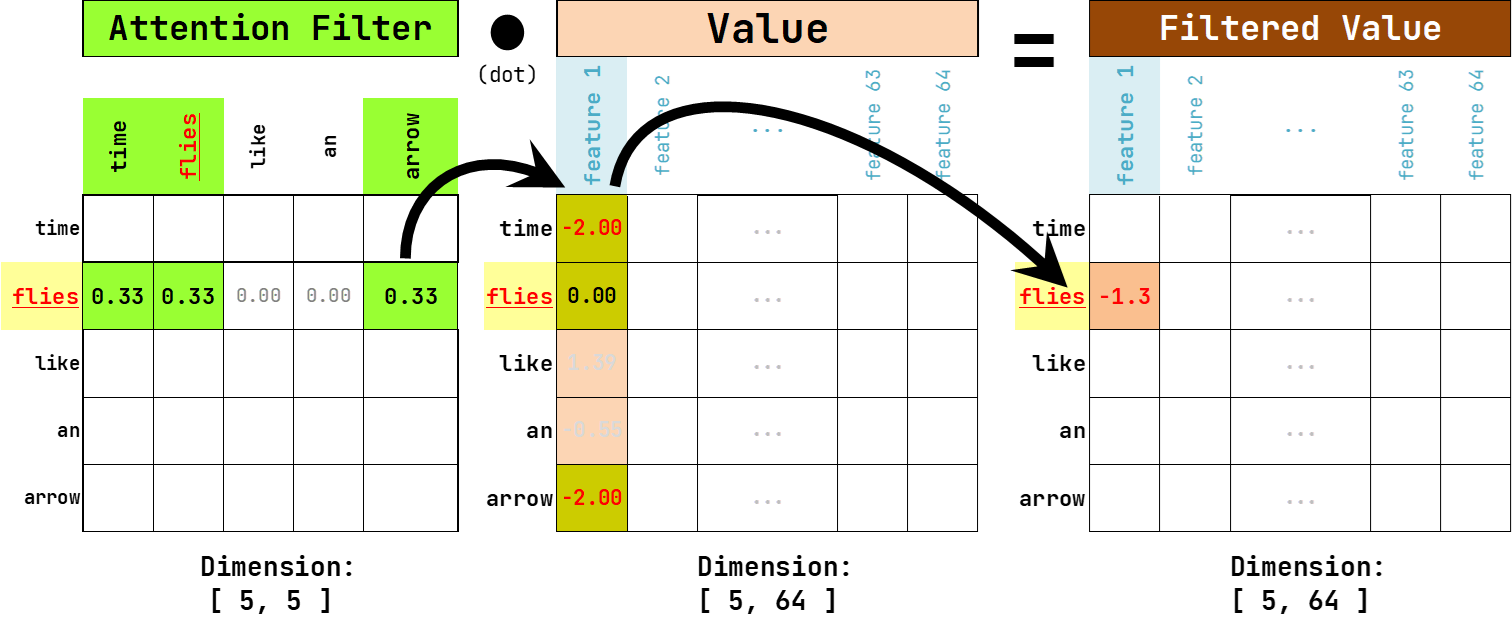
\includegraphics[width=0.9\textwidth]{Assets/filteredvalues1}
	\caption{\colorbox{brown}{\emph{Filtered Value}}: \emph{time flies like an arrow}}
	\label{filteredvalues1}
\end{figure}

It is assumed that the \colorbox{lime}{\emph{Attention Filter}} has identified the words \emph{time} and \emph{arrow} to be important context words for the word \emph{flies} in the sentence \emph{time flies like an arrow}.
The \colorbox{lime}{\emph{Attention Filter}} thus shows exemplary values of \textbf{0.33} for each of these context words and the word \emph{flies} itself, and a value of \textbf{0.00} for the remaining words \emph{like} and \emph{an}.

It is further assumed that the first column of the \colorbox{orange}{\emph{Value}} matrix represents a semantically interpretable feature that humans would describe as \emph{food-like} (like the column \emph{food} in the handcrafted feature table in Fig.\ref{fig:wordfeaturesmanually}).
If a given word in a wider sense has something to do with \emph{food}, it is assumed that the values in the first column of the \colorbox{orange}{\emph{Value}} matrix are positive, else zero or negative.
In Fig.\ref{filteredvalues1}, the exemplary \emph{food} feature values for the word \emph{time} and \emph{arrow} are \textbf{-2.00} as both words are assumed to have nothing to do with \emph{food}.
The exemplary \emph{food} feature value for the word \emph{flies} itself is assumed to be \textbf{0.00} (as some \emph{flies} might be edible insects and to make the point clearer).
The dot product of the 2nd row of the \colorbox{lime}{\emph{Attention Filter}} with the 1st column of the \colorbox{orange}{\emph{Value}} matrix so yields a value of \textbf{-1.3} at the 2nd row and 1st column of the \colorbox{brown}{\emph{Filtered Value}} matrix (see Fig.\ref{filteredvalues1}).


The 2nd row of the \colorbox{brown}{\emph{Filtered Value}} matrix already represents the contextualized or dynamic word embedding vector of the word \emph{flies} in the sentence \emph{time flies like an arrow}.
Whereas the \emph{food} feature value in the \colorbox{orange}{\emph{Value}} matrix for the word \emph{flies} was \textbf{0.00}, this value at the same coordinate in the \colorbox{brown}{\emph{Filtered Value}} matrix has changed to \textbf{-1.3}.
This change in the vector representation of the word \emph{flies} can be \underline{entirely attributed} to the negative \emph{food} feature value contributions coming from the words \emph{time} and \emph{arrow} in the \colorbox{orange}{\emph{Value}} matrix.

\paragraph{\emph{fruit flies like a banana}}
The same analysis is now done for the sentence \emph{fruit flies like a banana} shown in Fig.\ref{fig:filteredvalues2}.

\begin{figure}[H]
	\centering
	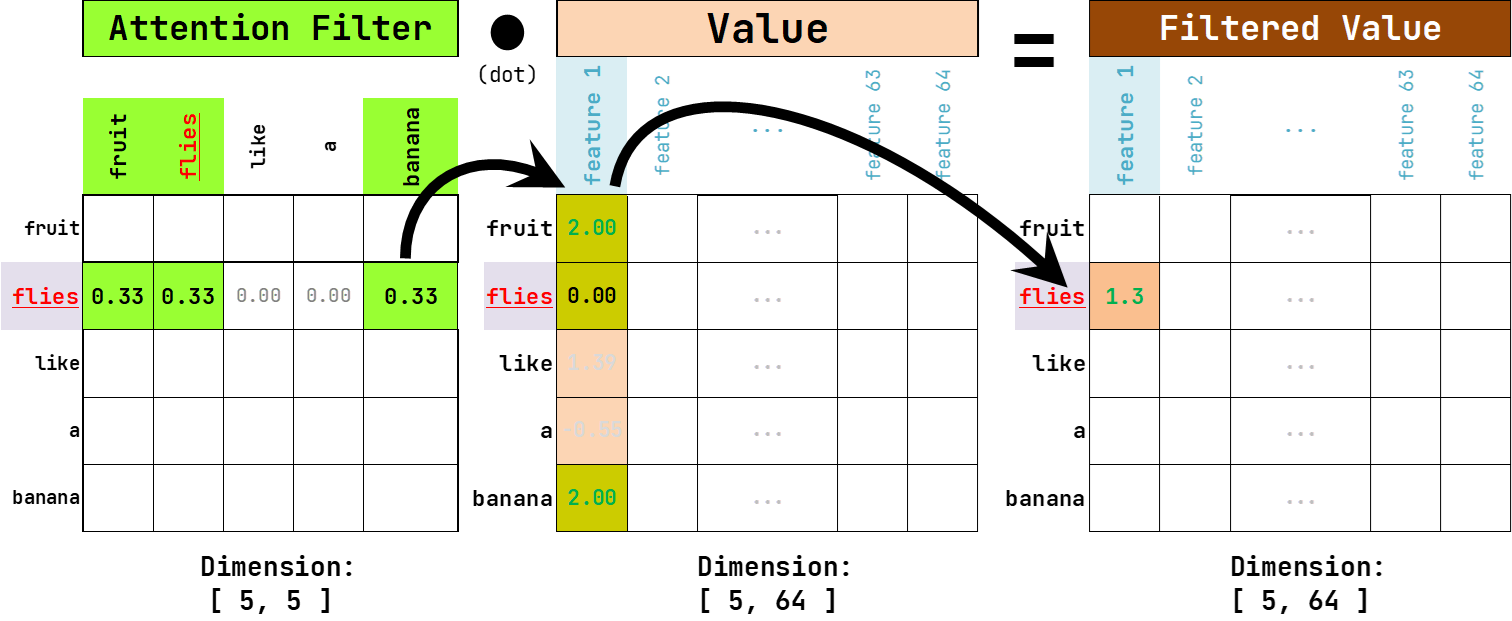
\includegraphics[width=0.9\textwidth]{Assets/filteredvalues2}
	\caption{\colorbox{brown}{\emph{Filtered Value}}: \emph{fruit flies like a banana}}
	\label{fig:filteredvalues2}
\end{figure}

Here, the assumption is that the \colorbox{lime}{\emph{Attention Filter}} has identified the words \emph{fruit} and \emph{banana} to be important context words for the word \emph{flies}, assigning the same exemplary values of \textbf{0.33} to them, like before.
The exemplary \emph{food} feature values for the word \emph{fruit} and \emph{banana} are now assumed to be \textbf{+2.00} as both words are strongly related to the idea of \emph{food}.
The exemplary \emph{food} feature value for the word \emph{flies} itself has not changed as it is indirectly coming from the static \emph{Input Embeddings}.
Every unique word (representation) in the \colorbox{orange}{\emph{Value}} matrix is the same for all sentences.
The dot product of the 2nd row of the \colorbox{lime}{\emph{Attention Filter}} with the 1st column of the \colorbox{orange}{\emph{Value}} matrix \textbf{now} yields a positive value of \textbf{+1.3} (see Fig.\ref{fig:filteredvalues2}), again coming from a value of \textbf{0.00} in the \colorbox{orange}{\emph{Value}} matrix.
This change in the vector representation of the word \emph{flies} in the \colorbox{brown}{\emph{Filtered Value}} matrix can be \underline{entirely attributed} to the positive \emph{food} feature value contributions coming from the words \emph{fruit} and \emph{banana} in the \colorbox{orange}{\emph{Value}} matrix.

\paragraph{\emph{Different embeddings for same word depending on context}}
The application of this principle to not only one column (here the \emph{food} feature column), but to all 64 columns of the \colorbox{orange}{\emph{Value}} and \colorbox{brown}{\emph{Filtered Value}} matrices, ensures that different semantic and syntactic aspects of word inter-dependencies are accounted for.
The \colorbox{brown}{\emph{Filtered Value}} matrix is where all the attention magic plays out.
Whereas the \colorbox{orange}{\emph{Value}} matrix can be considered a \textbf{static} word embedding, the \colorbox{brown}{\emph{Filtered Value}} matrix truly is a \textbf{dynamic} representation of words as it depends on the context words that are identified by the \colorbox{lime}{\emph{Attention Filter}} and that are different for every sentence.
The embedding vector of the word \emph{flies} in the \colorbox{brown}{\emph{Filtered Value}} matrix is different for the two sentences because the adjacent words to \emph{flies} are different and so is its context.\\
This means that \gls{Transformer}-based models can encode human language semantics and syntax much better than previous models.

%%%%%% Hallucination

\section{Is a \gls{gen-llm} all you need?}\label{sec:is-a-generative-llm-all-you-need?}
\paragraph{\glspl{gen-llm}}

A recent trend in \gls{nlp} seems to be the increasing use of \glspl{gen-llm}, like OpenAI's GPT models, for all kinds of \gls{nlp}-related tasks such as \gls{ner} or \gls{coref_resolution_definition}.
Instead of developing, pretraining or fine-tuning custom models using traditional programming languages, algorithms and datasets, researchers and practitioners seem to increasingly focus on engineering \glspl{prompt} to let \glspl{gen-llm} perform the task.

\paragraph{\gls{RAG} Systems}\label{par:rag-systems}
\gls{RAG} systems are sometimes added to such \glspl{gen-llm} in order to improve their accuracy.
\gls{RAG} stands for \emph{Retrieval Augmented Generation} and is a means to enrich a \gls{prompt} with relevant information.
Proprietary documents are typically chunked and loaded into a vector database to add context and information to the \gls{prompt}.
\gls{RAG} systems typically rely on vector similarity measures such as cosine similarity (see Section \ref{subsec:document-similarities}).
The text of a user question is converted to an embedding vector for which a similar embedding vector is searched in the vector database.
The text document with the highest cosine similarity is processed and formulated as an answer to the user's question.

\paragraph{The Hallucination problem}\label{par:hallucination}
Although \glspl{llm}, with contextual word embeddings at its core, have revolutionized the \gls{nlp}-world,
\gls{Hallucination}, or the presentation of false or misleading information as facts \cite{Hallucination}, still remains a problem and for some researchers is even inevitable \cite{hallucinationinevitable}.


\glspl{Hallucination} are often caused by the conflict between the user's intent and the characteristics of \glspl{llm}:

\begin{itemize}
\item Good \glspl{llm}, and good Machine Learning models in general, are supposed to \emph{generalize} well but are not supposed to \emph{memorize} their training data
\item \glspl{gen-llm} generate their text based on the highest probability for the next word
\item These probabilities hinge on the data fed to the \gls{llm} during training or retrieved from \gls{RAG}-systems
\end{itemize}

Generalization means that the \gls{llm} outputs text that fits learned patterns, but does not output the training (or \gls{RAG}) text itself.
Even if the training data was all true and factual (which is unlikely), the generated output text would most likely be different.
Even if a certain, factually correct text was part of the training data, an \gls{llm} ChatBot will most likely not return the same text.
Next word generation based on probabilities means, that of all candidate words the one word with the highest probability is taken, even if that probability itself is very low.

For a creative goal such as writing novels or poetry, this might not be a problem and often is a desired characteristic.
For the goal of retrieving or generating text that contains correct and accurate facts, this might be damaging as demonstrated by the \emph{ChatGPT-Lawyer}-case \cite{WebsiteChatGPTLawyer}, where a lawyer cited fake legal cases that were generated by ChatGPT.

Domain-specific training data and \gls{RAG}-systems can decrease \gls{Hallucination} rates, but not entirely.
A recent study \cite{hallucinationlegal} by Yale and Stanford researchers revealed that even domain-specifically trained, \glspl{gen-llm}
with extensive \gls{RAG}-systems attached to them, showed \gls{Hallucination}-rates of between 17 and 33 percent.

\paragraph{Questions in regard to LLMs}
Two of the questions for this project are driven by this problem.
The first question is:
\begin{center}
	\emph{Given the problem of hallucinations, how do \glspl{gen-llm} perform versus tradional methods on the task of information extraction?}
\end{center}
In the \emph{Information Extraction Pipeline}, different approaches will be studied, implemented in code and compared with each other.
This covers traditional rule-based and pre-trained \gls{ann} models, but also models based on \glspl{gen-llm}.\\

In the Knowledge Graph part, a ChatBot (\gls{graph-bot}) will be attached to the Knowledge Graph.
This is to elaborate on the question
\begin{center}
	\emph{Can Knowledge Graphs be used as an alternative to traditional RAG-systems?}
\end{center}
A recent research by Microsoft \cite{graphrag} does point in this direction, but does this also apply to this project and its data?\\

In the next chapter, the project and \emph{Information Extraction Pipeline} will start with extracting named entities.





\chapter{\gls{ner} - Named Entity Recognition}
A named entity is an object that can be referred to and tagged with a predefined entity class label to which the object belongs.
The most common entity classes and tags are \gls{per} for persons, \gls{org} for organizations, \gls{loc}
for geographical locations and \gls{gpe} for geopolitical entities.
The task of Named Entity Recognition (\gls{ner}) is to find \glspl{span} of text that constitute such entity classes or tags \cite{StanfordNLPNER}.

\section{Background}
This section will give an overview over the models that have been used previously and the current state-of-the-art models.
\subsection{Rule-Based Models}\label{subsec:rule-based-models}
Rule-based models were the earliest attempts to recognize named entities in text.
They often used lexical patterns, syntactic features, and domain-specific knowledge such as the following:

\begin{center}
\textit{\textbf{Rule}: If a token is capitalized and the next token is a noun, then the first token is likely a person name.}
\end{center}

While Machine Learning (see \ref{subsec:machine-learning-models}) or Deep Learning approaches (\ref{subsec:deep-learning-models})
dominate the academic debate and research, production use cases today still use hand-crafted rules and query techniques \cite{StanfordNLPNER} to find named entities.
One of the reasons for that is the ambiguity and similarity of entity names and types that confuses even the best \gls{ner} models available.
For instance, \textit{A.G. Edwards} could be both, a \gls{per} or an \gls{org} and the company \textit{Blue Shark} could be falsely identified as an animal.
Another reason is that in some use cases only certain entity types or already known entity names shall be found.
In such cases, it often makes sense to comb through a text with \gls{Regex} patterns or apply other handcrafted query strategies.

\subsection{Machine Learning Models}\label{subsec:machine-learning-models}
There are different types of Machine Learning models for the \gls{ner} task.
\subparagraph{Hidden Markov Models}
Hidden Markov Models or \glspl{HMM} \cite{StanfordNLPNER} are applied to sequences of observations and their respective hidden states.
In the field of \gls{ner}, the observations are the words in a text sequence and their hidden states are
the \gls{ner}-tags such as \gls{per} or \gls{loc} to be predicted.

\begin{figure}[H]   %[h] puts picture right here. 't' stands for to, 'b' stands for bottom
    \centering
    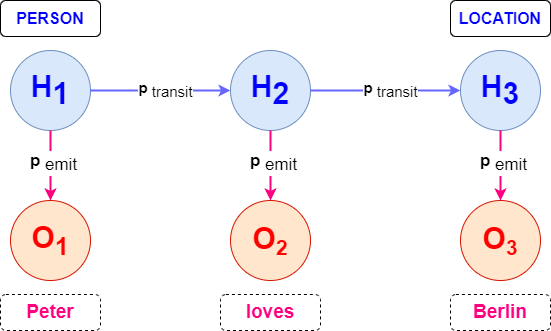
\includegraphics[width=0.5\textwidth]{Assets/HMM}
    \caption{\gls{HMM}: transition/emission probabilities: \textbf{p}\textsubscript{trans}, \textbf{p}\textsubscript{emit}}
    \label{fig:HMM}
\end{figure}

\subparagraph{Conditional Random Fields}
\glspl{CRF} \cite{StanfordNLPNER} belong to the family of \glspl{HMM} and try to address the shortcomings of \glspl{HMM} when it comes to text sequences.
The first problem with a standard \gls{HMM} is that transition and emission probabilities (Fig.\ref{fig:HMM}) are static whereas in text, they are dynamic.
The emission probability that the name of a \gls{per} is \textit{Peter} depends on the context and therefore is dynamic as is the probability that a \gls{loc} comes two words after a \gls{per}.
The second problem is that dependencies are limited in a standard \gls{HMM} meaning that previous hidden states have no direct impact on observations farther away in the sequence.
In a text sequence though, the \gls{ner} tag of the first word in a sentence might have an impact on a word that sits at the end of a sentence.

\begin{figure}[H]   %[h] puts picture right here. 't' stands for to, 'b' stands for bottom
    \centering
    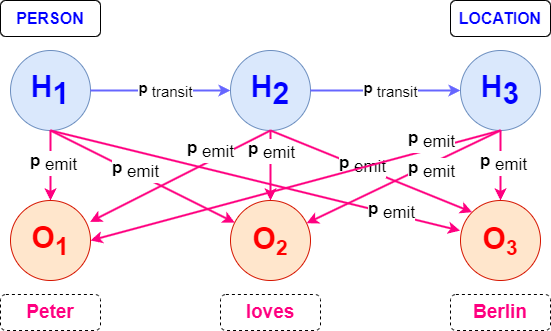
\includegraphics[width=0.55\textwidth]{Assets/CRF}
    \caption{Linear Chain \gls{CRF}}
    \label{fig:CRF}
\end{figure}
A linear chain \gls{CRF} (Fig.\ref{fig:CRF}) overcomes this limitation by allowing emission probabilities from a hidden state (i.e. a \gls{ner} tag) to previous and subsequent observations (i.e. words) but, to avoid computational complexity, prohibits transition probabilities to previous and subsequent hidden states.
The network of emission probabilities and the mapping from the words to the respective \gls{ner} tag is modeled via \textit{\textbf{k}} different feature functions \textbf{f}\textsubscript{j}:

\begin{equation}
f(H_i): \sum\limits_{j=1}^{k} \vec{\textbf{w\textsubscript{j}}} \cdot f_j(O_i, H_{i-1}, H_i, i)  \label{eq:crf1}
\end{equation}

Each feature function has different hidden-state-to-observation \textit{connections} and the model is trained with all vectors \textit{\textbf{w\textsubscript{j}}} as a trainable matrix.
The conditional probability of a certain state \textit{H\textsubscript{i}} (or \gls{ner}-tag) given the observation \textit{O\textsubscript{i}} (or word) and a normalization factor \textit{Z} is calculated by:

\begin{equation}
p(H_i \;| \;O_i) = \frac{1}{Z} \cdot \exp \sum\limits_{l=1}^{n_{words}} \sum\limits_{j=1}^{k} \vec{\textbf{w\textsubscript{j}}} \cdot f_j(O_i, H_{i-1}, H_i, i)  \label{eq:crf2}
\end{equation}

Words as input to a \gls{CRF} model can come in the form of an encoded index from a lookup table or as embedded word vectors \cite{StanfordNLPNER}.

\subsection{Deep Learning Models}\label{subsec:deep-learning-models}

The advent of \glspl{llm} also changed the field of \gls{ner} fundamentally.
Today all leading \gls{ner}-models are based on \gls{Transformer} architectures \cite{leaderboard-ner}.
\glspl{Transformer}, or in more general terms, \gls{ann}-based models can be distinguished between pre-trained models and \glspl{gen-llm}.
Whereas pre-trained models are supervised general purpose \glspl{ann} that are fine-tuned for a specific \gls{ner} task,
\glspl{gen-llm} use the decoder part of a \gls{Transformer} architecture to generate text in response to a \gls{ner}-specific \gls{prompt} request.

\paragraph{Pre-Trained Models}
There are multiple pre-trained models available such as bert-base-NER \cite{bertbaseNER} or NER-BERT \cite{nerbert}, but the one model that stands out in terms of performance and multilingual support is GliNER \cite{gliner}.
GliNER is a light-weight \gls{Transformer} model based on the deBERTa-v3 \cite{deberta} architecture with additional layers for \gls{span} and entity representations.
It was trained with texts from numerous domains and thousands of entity types \cite{gliner} which allows custom entity labels beyond the ones typically found in \gls{ner} models (i.e. \gls{org}, \gls{per}, \gls{loc}, etc.).
GliNER maximizes a combined \gls{token}-\gls{span}-Entity embedding matching score in a computationally efficient way to achieve an O(n log n) complexity.
Because it is available as a spacy wrapper module, it can easily be added to a spacy pipeline.

spacy itself until recently also had a well-performing \gls{ner} component in their pre-trained pipelines (i.e.\emph{en\_core\_web\_sm}, etc.) but performance-wise had to surrender to more recent and specialized models such as GliNER.

GliNER’s multilingual spacy wrapper was used in the project and later compared against a traditional \gls{Regex} model.

\paragraph{\glspl{gen-llm}}\label{par:gpt-ner}
Besides using \glspl{llm} such as the ones from OpenAI directly by sending \gls{prompt} requests, there are also dedicated architectures and indirect ways to extract the named entities from text.

Wang et al \cite{gptner} in 2023 introduced GPT-NER that transforms the \gls{span} labeling task into a text generation task.
For instance, the task of finding \gls{loc} entities in the input text \emph{Columbus is a city}, is transformed to generate the text sequence \emph{@@Columbus\#\# is a city}, where the special \glspl{token} @@ and \#\# surround the entity to be extracted \cite{gptner}.
Before returning the result to the user, the \gls{prompt} also asks the \gls{gen-llm} to self-verify its findings thus decreasing the problem of \glspl{Hallucination}.
The text is then searched for the special \glspl{token} and the model returns the entity in between them.

In the same year, Ashok and Lipton \cite{promptner} introduced PromptNER, which focuses on a specific set of entity types.
The \gls{prompt} provides the model with annotated examples and forces it to justify its findings with the entity type definitions provided.

Most other approaches that I came across, use \glspl{gen-llm} for \gls{ner} in a similar way or concentrate on specific industries or domains.

\section{Code-Implementation}\label{sec:code-implementation}

\subsection{Implementation of Pre-Trained Model}
As GliNER \cite{gliner} is available as a registered spacy plugin (see Section \ref{par:spacy-plugin}), the implementation of it in a spacy pipeline is straightforward.
The name of the plugin is just referenced in the spacy function \emph{enable\_pipe("gliner\_spacy")} within the \emph{api\_gliner()} function (see Python-Code \ref{code:spacy-add-gliner})

\begin{listing}[H]
    \captionof{listing}{api\_gliner()}
    \inputminted[
    firstline=149,
    lastline=158,
    firstnumber=149,
    ]{python}{/media/rainergo/PROJECTS/UASFRA-MS-Thesis/src/B_spacy_pipeline/spacy_pipe_build.py}
    \label{code:spacy-add-gliner}
\end{listing}

and this function is then added to the \emph{build\_pipe()} method (see line 110 of Python-Code \ref{code:spacy-add-gliner-function}) in the \emph{SpacyPipeBuild} class, as outlined in Section \ref{subsec:usage}.

\begin{listing}[H]
    \captionof{listing}{build\_pipe()}
    \inputminted[
    firstline=99,
    lastline=113,
    firstnumber=99,
    ]{python}{/media/rainergo/PROJECTS/UASFRA-MS-Thesis/src/B_spacy_pipeline/spacy_pipe_build.py}
    \label{code:spacy-add-gliner-function}
\end{listing}

\subsection{Implementation of Rule-Base Model}
\paragraph{\gls{Regex}}
As stated previously, in some use cases it might make sense to use rule-based models (see \ref{subsec:rule-based-models}) for \gls{ner}.
Pre-trained \glspl{llm}, that incorporate syntactical and semantic information in their embeddings, are required if entity names are unknown and must be determined in a probabilistic way.
As the company names are provided in advance in this project, rule-based methods such as \glspl{Regex} can be tried for \gls{ner}.

For \gls{Regex} to find desired company names in a text, \gls{Regex} patterns need to be created first.

\gls{Regex} patterns can consist of multiple components and these components can either be mandatory or optional.
One such example is the following:

\begin{center}
\textbf{(Hello)\textbackslash s?(World)*}
\end{center}

The first capturing group contains the word \textit{Hello} and the second the word \textit{World}.
The second group and the space in between the words are optional as these terms are followed by an asterix or a question mark which are \emph{quantifiers}.
The first group is mandatory as an \emph{optional quantifier}, such as ?, *, \{0, n\}, is missing.
In this example, the expression \emph{Hello} or \emph{Hello World} would match the pattern, but the expressions \emph{World} or \emph{Hi World} would not.

Company names can consist of one or multiple words.
To distinguish company names from each other and from non-company names, the company name must be recognizable and distinct.
If a company name consists of more than one word, the central question for \gls{Regex} patterns is which words in the company name must be mandatory and which can be optional.
Let’s consider the following company name example:

\begin{center}
\textbf{Deutsche Telekom AG}
\end{center}

A \gls{Regex} pattern must include at least the first two words combined as the words \emph{Deutsche} and \emph{Telekom} alone are not distinct and are commonly used words.
Let’s consider another example:

\begin{center}
\textbf{Apple Inc.}
\end{center}

Here, the same logic applies: The pattern must include the legal term \emph{Inc.} as otherwise the pattern could find a fruit instead of the company \emph{Apple} whereas in the next example the legal term could be optional:

\begin{center}
\textbf{2CRSI S.A.}
\end{center}

The term \emph{2CRSI} itself is so significant and distinct, that the probability of the same term referring to something else than the given company, is very low.

The optionality of a word in a company name is important for two reasons:
\begin{itemize}
  \item Company names are typically fully mentioned at the beginning of a text but in later sentences might be referred to with just one part of their name.
  \item Company mentions could also be part of a noun term.
\end{itemize}

Let’s consider the following sentences:

\begin{center}
\small{\textit{\underline{ACCENTRO Real Estate AG} today published their better than expected earnings.
\underline{Accentro} had a good first quarter, the \underline{Accentro-stock} climbed 3\% on the stock exchange.}}
\end{center}

A \gls{Regex} pattern that has no optionality for the words \emph{Real Estate AG} would only match the first company mention, but would not match the second and third.
So a good \gls{Regex} pattern might look like this:

\begin{center}
\footnotesize{\textbf{(?:\textbackslash bACCENTRO\textbar Accentro\textbackslash b)\textbackslash s*(?i:\textbackslash bReal\textbackslash b)?\textbackslash s*(?i:\textbackslash bEstate\textbackslash b)?\textbackslash s*(?i:\textbackslash bAG\textbackslash b)?}}
\end{center}

The central word \emph{Accentro} could be upper or title cased, the words \emph{Real}, \emph{Estate}, \emph{AG} are optional and their case could be any.
The \emph{\textbackslash b} means beginning and end of a word and the spaces in between the words are optional.
With such a pattern, all three mentions of the company name in the above example will be matched.

\paragraph{Implementation Details}
As the number of companies to be searched for exceeds 2500, manually creating such regular expression patterns would be very time-consuming.
The function

\begin{center}    
\emph{create\_and\_save\_entity\_patterns()}
\end{center}

in the module \emph{spacy\_input} in the \emph{B\_spacy\_pipeline} folder is particularly dedicated to algorithmically transform company names to \gls{Regex} patterns.


They work as follows:
\begin{enumerate}
  \item The function splits the company name into a list of words.
  \item Each word in this list is classified into one of the following classes:
    \subitem \textbf{Binding}: A conjunction term that links two other words such as \emph{and}, \emph{+}, \emph{-}, \emph{\&} like in \emph{Smith \& Wesson}, \emph{Busch+Lombard AG} or \emph{Basic-Fit N.V.}, etc.
    \subitem \textbf{Person Name Initials} such \emph{A.G.} in \emph{A.G. Edwards}.
    \subitem \textbf{Person Names}: For that, a list of 5000 German and English common first and last names are searched for.
    \subitem \textbf{Legal Terms} such as \emph{AG}, \emph{NV}, \emph{GmbH}, etc for which a legal term list was compiled.
    \subitem \textbf{Industry Hints}: Words that give a hint to the industry the company operates in such as \textbf{buildings}, \textbf{capital}, \textbf{carbon}, \textbf{care}, \textbf{casino}, \textbf{catering}, etc.
    \subitem \textbf{Number Terms} such as 11880 in \emph{11880 Solutions}.
    \subitem \textbf{Significantly Cased Words} such as \emph{SUESS} or \emph{MicroTec}
    \subitem \textbf{Number and Letter Words} such as \emph{4imprint} in \emph{4imprint Group plc.}.
    \subitem \textbf{Articles} such as \emph{The} in \emph{The New York Times}.
    \subitem \textbf{Common Words}: If the word is commonly used according to a list of \emph{5000 most common words} in English and German or if the word is in a list of common company name prefixes and suffixes such as \emph{Global} or \emph{Group}.
    \subitem \textbf{Unknown Words}: Words that do not belong to one of the other classes above.

  \item Once all words of a company name are classified, combination patterns of up to five words are created.
\end{enumerate}

The classification task often is carried out with the help of regular expression patterns itself and Python string functions.\\

As a three-word example, let’s assume the company name is:

\begin{center}
\textbf{4imprint Group plc.}
\end{center}

In the first step, the company name gets split into: [\emph{4imprint}, \emph{Group}, \emph{plc}].
In the second step, each of the three words is classified: \emph{4imprint} is classified as a \emph{Number and Letter word}, \emph{Group} is classified as a \emph{Common Word} and \emph{plc} is classified as \emph{Legal Term}.

\emph{Number and Letter Words} are considered unique and distinct so all other words in that company name can be optional.
The resulting regular expression pattern is:

\begin{center}
\footnotesize{\textbf{(?:\textbackslash b4imprint\textbar4Imprint\textbackslash b)\textbackslash s*(?i:\textbackslash bGroup\textbackslash b)?\textbackslash s*(?i:\textbackslash bplc\textbackslash b)?}}
\end{center}

Let’s consider a four-word example:

\begin{center}
\textbf{Advanced Bitcoin Technologies AG}
\end{center}

In the first step, the company name again gets split into: [\emph{Advanced}, \emph{Bitcoin}, \emph{Technologies}, \emph{AG}]
In the second step, \emph{Advanced} is classified as a \emph{Common Word} as is the word \emph{Technologies}.
\emph{Bitcoin} is classified as an \emph{Industry Hint} and \emph{AG} as a \emph{Legal Term}.
No word from these classes is considered unique and distinct, but the legal classifier is not needed as there is more than one word in the company name.
So the algorithm determines that the first three words are mandatory in the \gls{Regex} pattern and the legal term is optional:

\begin{center}                                                                                                                                                                                                              
\footnotesize{\textbf{(?:\textbackslash bAdvanced\textbackslash b)\textbackslash s*(?:\textbackslash bBitcoin\textbackslash b)\textbackslash s*(?:\textbackslash bTechnologies\textbackslash b)\textbackslash s*(?i:\textbackslash bAG\textbackslash b)?}}
\end{center}


\paragraph{Pattern Naming and Multithreading}
The patterns are saved as \emph{JSONL}-files and are later loaded by a spacy pipeline component that tries to find matches for the patterns in the text.
As the number of companies and thus the number of patterns exceeds 2500, two questions arise:

\begin{enumerate}
    \item How can matches of patterns be mapped to the individual company identifiers and names?
    \item How can over 2500 patterns be efficiently run against each text?
\end{enumerate}

Each \gls{Regex} pattern gets a name that is derived from the company’s unique identifier which is the company stock ticker symbol.


The function \emph{symbol\_to\_groupname\_convert()}
\begin{listing}[H]
    \captionof{listing}{symbol\_to\_groupname\_convert()}
    \inputminted[
    firstline=62,
    lastline=77,
    firstnumber=62,
    ]{python}{/media/rainergo/PROJECTS/UASFRA-MS-Thesis/src/B_spacy_pipeline/spacy_input.py}
    \label{code:symbol-to-groupname-convert}
\end{listing}
first converts the company symbol to a regular expression name which is then prefixed to the pattern that was created above.

For instance: The stock ticker symbol for the company \emph{Advanced Bitcoin Technologies AG} is \emph{ABT.DU}.
The function converts this to a pattern-eligible name which is \emph{SYMB\_ABT\_DOT\_DU} and with it prefixes the regular expression pattern that was created above:

\begin{center}                                                                                                                                                                                                                                                   
\footnotesize{\textbf{(?P\textless SYMB\_ABT\_DOT\_DU\textgreater (?: \break (?:\textbackslash bAdvanced\textbackslash b)\textbackslash s*(?:\textbackslash bBitcoin\textbackslash b)\textbackslash s*(?:\textbackslash bTechnologies\textbackslash b)\textbackslash s*(?i:\textbackslash bAG\textbackslash b)?))}}
\end{center}                                                                                                                                                                                                                                                     

A match against this pattern returns a Python \emph{re match object} that, among other information, contains the pattern’s name.
The pattern’s name then can be re-converted to the company symbol which is attached as extension to the matching \gls{span} or \gls{token} in the Doc-object of the spacy pipeline.

To make this process computationally efficient, the matching algorithm is run concurrently.
The function \emph{run\_re\_finditer\_concurrently()} runs the Python re function \emph{finditer} in parallel and the spacy pipeline component \emph{OwnRegexSearch} applies this concurrent function to each article text:

% Importing code from Python file and overwrite global minted settings

\begin{listing}[H]
    \captionof{listing}{run\_re\_finditer\_concurrently()}
    \inputminted[
    firstline=8,
    lastline=20,
    firstnumber=8,
    ]{python}{/media/rainergo/PROJECTS/UASFRA-MS-Thesis/src/G_utils/concurrency.py}
    \label{code:run-re-finditer-concurrently}
\end{listing}

This match algorithm, that runs over 2500 patterns on each article text, on my standard machine only takes around 500 milliseconds on average per text to execute.

\paragraph{Comparing Rule-Based vs. Pre-Trained vs. \glspl{gen-llm}}
With 500 milliseconds per text, the rule-based method with \gls{Regex} is approximately as fast as the respective GliNER component in spacy’s pre-trained pipeline.
The \gls{Regex} algorithm does not find all companies in the text and is particularly sensitive to misspelled company names, too little optionality in the \gls{Regex} pattern or if company names only consist of one, very common word.


But in most cases, it is as accurate as spacy’s pre-trained GliNER pipeline component and in some cases, particularly if the company name is peculiar and can be confused with subjects from other domains, it is more accurate.
Some shortcomings of the regex approach can be cured if non-working patterns are manually adjusted.
For instance: The company name
\begin{center}
    \textbf{Schott Pharma AG \& Co. KgaA}
\end{center}
contains the person name \emph{Schott} which is uncommon and thus not found in the existing list of person names for the classification task in the \emph{create\_and\_save\_entity\_patterns()} function.
The name \emph{Schott} also starts with a capital letter and is thus considered unique and distinct for which the algorithm allows the other words in the company name to be optional.
The \gls{Regex} pattern could be adjusted by manually adding the name \emph{Schott} to the list of common person names or by requiring the word \emph{Pharma} to be mandatory.

\subsection{Implementation of \gls{gen-llm} model}
For the sake of comparing different approaches, I also tried a \gls{gen-llm} for the \gls{ner} task.
Asked to find named entities in a text, ChatGPT using the OpenAI 4o-mini model with a simple \gls{prompt}, already found most of the entities in a sample text:

\begin{figure}[H]   %[h] puts picture right here. 't' stands for to, 'b' stands for bottom
    \centering                                                                                                                     
    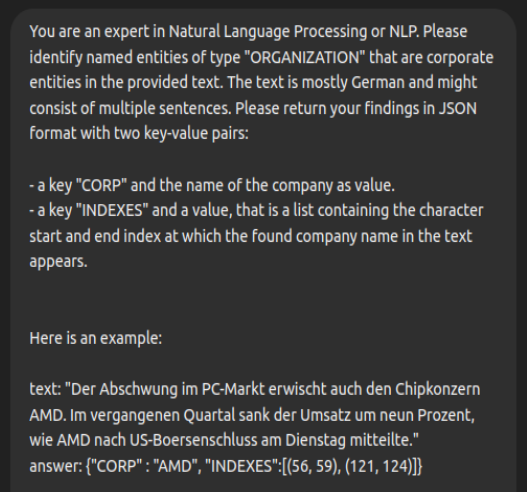
\includegraphics[width=0.9\textwidth]{Assets/chatgpt11}
    \caption{ChatGPT \gls{ner} \gls{prompt} - Part 1}
    \label{fig:chatgpt11}
\end{figure}
\begin{figure}[H]   %[h] puts picture right here. 't' stands for to, 'b' stands for bottom
    \centering
    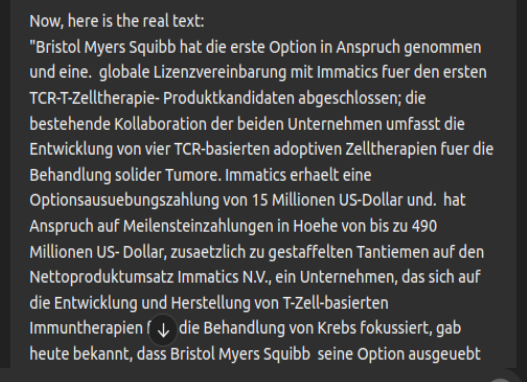
\includegraphics[width=0.9\textwidth]{Assets/chatgpt12}
    \caption{ChatGPT \gls{ner} \gls{prompt} - Part 2}
    \label{fig:chatgpt12}
\end{figure}

\begin{figure}[H]
    \centering                                                  
    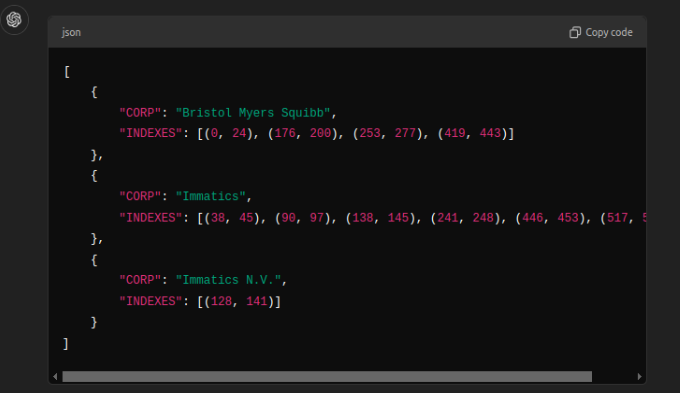
\includegraphics[width=0.9\textwidth]{Assets/chatgpt2}
    \caption{ChatGPT JSON Response}
    \label{fig:chatgpt2}
\end{figure}

But this \gls{gen-llm}-approach for \gls{ner} was inferior to the rule-based \gls{Regex} approach because:

\begin{itemize}
\item It found less entities.
\item It found entities that were not searched for.
\item The latency was higher as the request had to be sent to the OpenAI server first.
\item The position indexes for the found entities were all wrong so locating them would have required an extra step or the usage of OpenAI function tools which would have increased the latency even further.
\item It was more costly as OpenAI charges fees for using their \glspl{llm}.
\item The results were very volatile and unstable as they differed from request to request.
\end{itemize}

Some of these shortcomings can probably be cured by:
\begin{itemize}
\item fine-tuning the \gls{prompt}.
\item providing more few-shot examples.
\item using function tools that are available from most \gls{llm}-providers such as OpenAI.
\item providing a list of entities that shall be searched for.
\item using local, open-source \glspl{llm} and frameworks such as Llama3 \cite{llama3} running on Ollama \cite{ollama} installed on a local machine.
\end{itemize}
Nevertheless, the rule-based approach with \gls{Regex} already delivered very good results and in my assessment is best suited if the company names are given.
This would change if they were not given as then the creation of \gls{Regex} patterns was not possible and a choice would need to be made between a pre-trained and fine-tuned model or a \gls{gen-llm}-approach.

\subsection{Information Extraction Pipeline}
After the \gls{ner} component has run, the spacy pipeline has attached the found company information to the respective custom extensions:
\begin{figure}[H]   %[h] puts picture right here. 't' stands for to, 'b' stands for bottom
    \centering
    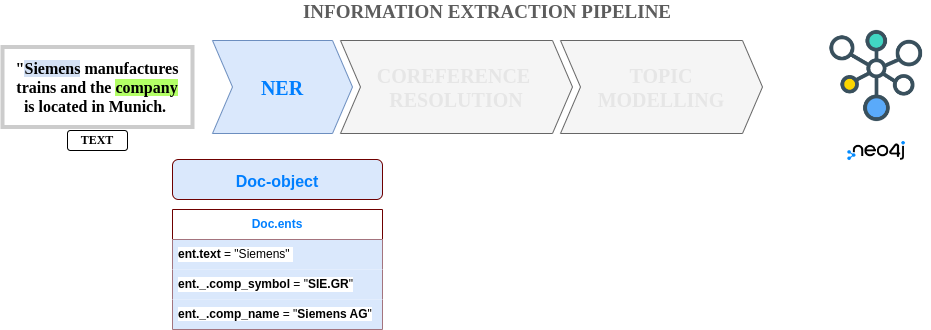
\includegraphics[width=0.85\textwidth]{Assets/pipelineNER}
    \caption{spacy pipeline after \gls{ner} component}
    \label{fig:pipeNER}
\end{figure}

\chapter{\gls{coref_resolution_definition}}\label{ch:coreference-resolution}


\section{Background}\label{sec:background}
In linguistics, \gls{coref_definition} occurs when two or more expressions refer to the same person or thing \cite{Coreference}.
In the sample sentence of Fig.\ref{fig:coreferences}, the expression \emph{he} refers to a \gls{per} with the name \emph{Philip} and the word \emph{it} refers to the musical instrument \emph{bass}, a thing.

\begin{figure}[H]   %[h] puts picture right here. 't' stands for to, 'b' stands for bottom
    \centering
    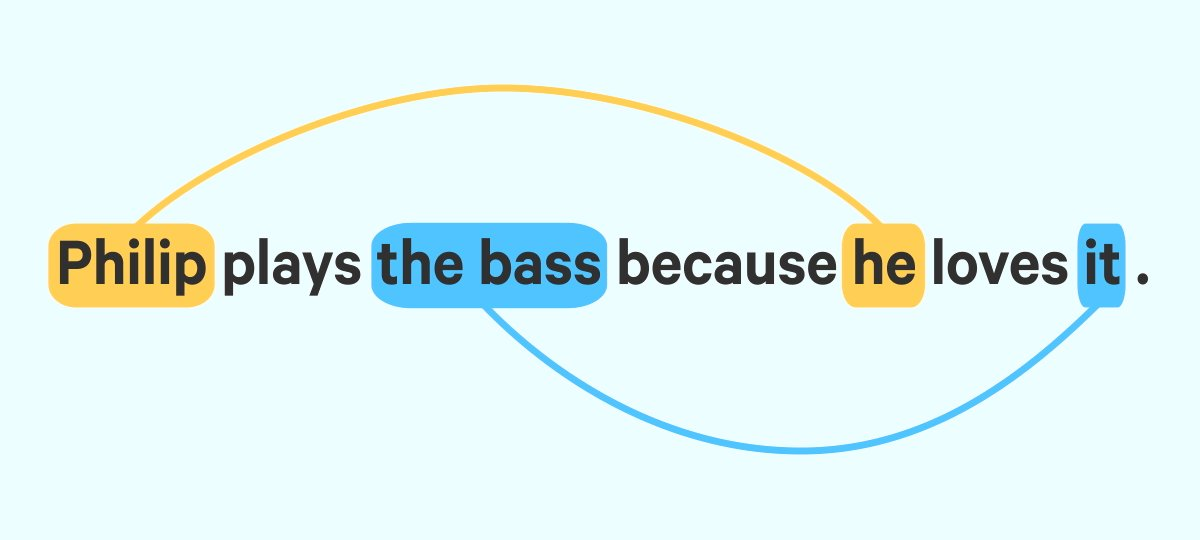
\includegraphics[width=0.7\textwidth]{Assets/spacycorefpic}
    \caption{Coreferences. Image from: \cite{spacy}}
    \label{fig:coreferences}
\end{figure}

\gls{coref_resolution_definition} is considered one of the most challenging tasks in \gls{nlp} and until recently was deemed an unsolved problem \cite{CorefResIsHard}.
The fundamental problem is the complex and ambiguous nature of natural language text, the requirement for a deep language understanding and the use of background knowledge in detecting \glspl{coref_definition} \cite{CorefResIsHard}.


\subsection{Definitions}\label{subsec:definitions}
In the sample sentence of Fig.\ref{fig:coreferences}, there are four \glspl{coref_mention} of which three are \glspl{token} [\emph{Philip, he, it}] and one is a \gls{span} [\emph{the bass}] consisting of more than one \gls{token}.
\glspl{coref_mention} often consist of long \glspl{span} such as \emph{The New York Times} or \emph{Bayerische Motoren Werke AG}.
Finding \glspl{coref_definition} in a text thus often is considered a \gls{span}-based task.
The \gls{coref_mention} \emph{Philip} is the \gls{coref_antecedent} for the \gls{coref_mention} \emph{it}.
As the name \emph{Philip} comes before \emph{it}, \emph{it} is the \gls{anaphora} for \emph{Philip}.
If \emph{Philip} came after \emph{it}, one would usually refer to \emph{it} as \gls{cataphora}.
The sample sentence has two \glspl{coref_cluster} or \gls{coref_definition} chains: [\emph{Philip, he}], [\emph{the bass, it}].

\subsection{Methods}\label{subsec:methods}
\subparagraph{Mention Detection}
The first step to detect \glspl{coref_definition} is \gls{coref_mention} detection \cite{StanfordNLPCoref}.
Earlier methods used grammatical parsers and named entity taggers on the text and, based on that, extracted
\glspl{span} that meet certain criteria as \gls{coref_mention}-candidates.
More recent \gls{coref_mention} detection systems go even further and extract literally all \gls{ngram} \glspl{span}
of \glspl{token} or words up to N=10, regardless of their grammatical attributes \cite{StanfordNLPCoref}.
Due to the computational complexity of this approach of
\begin{equation}
    O(number\_of\_tokens^4)
\end{equation}
for N=2 (Bi-Grams) \cite{CorefEndToEnd}, there is a need to filter out unlikely \glspl{span}.

\subparagraph{Rule Based Methods}
Earlier systems used rules to filter out non-coreferential pronouns like \emph{it} in sentences such as \emph{\underline{It} is likely that ...}.
These rule-based systems relied on regular expressions, dictionaries of key-verbs/-adjectives, \gls{pos} and \gls{ner} tags and other grammatical or syntactical rules.
Rule-based systems, however, generally underperform more modern systems that incorporate a learning process \cite{StanfordNLPCoref}.

\subparagraph{Feature Based Methods}
The next step thus were standard Machine Learning models that used decision trees, support vector machines and binary classifiers \cite{CorefSurvey}.
Theoretically, such models are capable to not only identify potential \glspl{coref_mention} but also whether such \glspl{coref_mention} are indeed \glspl{coref_definition}.
One common approach of such Classifiers is to implement a \emph{Mention-Pair-Architecture} that predicts if a given \gls{span} pair of an \gls{anaphora} and an \gls{coref_antecedent} are \glspl{coref_definition} or not \cite{StanfordNLPCoref}.
Another Classifier architecture type is the \emph{Mention-Rank-Architecture} that chooses the highest-scoring \gls{coref_antecedent} for each \gls{anaphora}.
\emph{Entity-based architectures} enhanced their feature set by adding \gls{coref_mention}-distances, syntactic, symantic, rule-based and lexical attributes to predict if a \gls{token} belongs to a certain \gls{coref_cluster} \cite{ClarkManning2015}.

Nevertheless, correctly detecting co-referential \glspl{coref_mention} remained difficult, mainly due to the model's lack for a deep language understanding \cite{StanfordNLPCoref}.

\subparagraph{Neural Network Based Methods}
A major breakthrough came with the advent of \glspl{llm} as contextual embeddings allowed to semantically compare \glspl{coref_mention}.
Consider the following phrases:

\begin{center}
    1: \textbf{Make a payment! You can make [it] in advance.} [anaphoric]
\end{center}
\begin{center}
    2: \textbf{Go west! You can make [it] in Hollywood.} [non-anaphoric]
\end{center}
\begin{center}
    Idea based on: \cite{StanfordNLPCoref}
\end{center}

Whereas the \emph{it} in the second phrase is non-anaphoric and part of the idiom \emph{make it}, the \emph{it} in the first phrase is anaphoric and refers to a \emph{payment}.
With contextual word-embeddings, the vectors for \emph{payment} and \emph{it} ideally should be similar in the first sentence whereas the vector for \emph{it} in the second sentence should significantly differ to any other word vector in that phrase.
The capability to detect the \glspl{coref_mention} \emph{payment} and \emph{it} as \glspl{coref_definition} should thus increase with contextual word embeddings.


\section{Models}\label{sec:models}
\gls{coref_definition} models can also be distinguished into three classes: Rule-Based, Pre-Trained and \gls{gen-llm} models.
As rule-based models factually are non-existent nowadays, the focus in the following chapter will be on Pre-Trained and \gls{gen-llm} models.

\subsection{Pre-Trained Models}\label{subsec:pre-trained-models}
\paragraph{Research}
All descriptions of the currently most performant pre-trained \gls{coref_definition} models are laid out in publicly available research papers.
Unfortunately, not all models are implemented in code and easily available as Python package.
This includes the two currently most performing \cite{CorefEvaluation} pre-trained \gls{coref_definition} models by Google Research \cite{CorefSeq2Seq} and Vladimir Dobrovolskii \cite{CorefDobrovolskii}.
As the model training of unimplemented \gls{coref_definition} research papers would go beyond the scope of this thesis,
I will shortly describe only those research papers for which a pre-trained Python package exists.

\subparagraph{e2e: End-to-end Neural \gls{coref_resolution_definition}}
In 2017, Lee et al.\cite{CorefEndToEnd} proposed an LSTM \cite{LSTM} model with a \emph{Mention-Rank-Architecture} where parsers and taggers are not required.
The model consists of two parts as shown in Fig.\ref{fig:e2e1} and \ref{fig:e2e2}:

\begin{figure}[H]   %[h] puts picture right here. 't' stands for to, 'b' stands for bottom
    \centering
    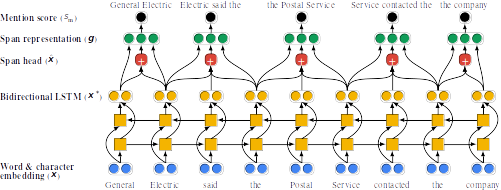
\includegraphics[width=1.0\textwidth]{Assets/e2e1}
    \caption{End-to-end Neural \gls{coref_resolution_definition}: Part 1}
    \label{fig:e2e1}
\end{figure}

In the first part (Fig.\ref{fig:e2e1}), the LSTM calculates \gls{span}-embeddings and assigns corresponding \gls{coref_mention} scores.
e2e is a supervised model trained with hand-labeled data.
Only the top M-ranked \glspl{span} with the highest \gls{coref_mention} scores are considered potential \glspl{coref_mention} and are further processed.
The concatenation of the \gls{token} embedding vectors creates the contextual \gls{span}-representation vectors.

\begin{figure}[H]   %[h] puts picture right here. 't' stands for to, 'b' stands for bottom
    \centering
    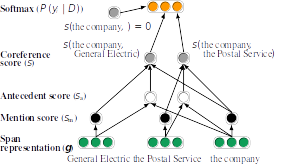
\includegraphics[width=0.7\textwidth]{Assets/e2e2}
    \caption{End-to-end Neural \gls{coref_resolution_definition}: Part 2}
    \label{fig:e2e2}
\end{figure}

In the second part of the model in Fig.\ref{fig:e2e2}, \emph{Antecedent scores} are computed from pairs of \gls{span}-representations.
The final \gls{coref_definition} \emph{score} is computed by summing the two \gls{coref_mention} \emph{scores} of the \glspl{span} and their pairwise \emph{Antecedent score}.
This calculation method avoids the computational inefficient evaluation of all (non-filtered-out) \gls{span} pairs and ensures, that the \gls{span}-pairs with the highest similarity yield the highest \gls{coref_definition} \emph{score}.

\subparagraph{c2f: Higher-order \gls{coref_resolution_definition} with Coarse-to-fine Inference}
In 2018, Lee et al. further improved their own model by changing the inference procedure of the \emph{Mention-Rank-Architecture}\cite{CorefCoarseFine} to refine \gls{span} representations.
This improved both, the computational complexity and the performance of the model.

\subparagraph{BERT for \gls{coref_resolution_definition}}
In 2019, Joshi et al. \cite{CorefWithBert} reused the \emph{Mention-Rank-Architecture} of Lee et al.\cite{CorefEndToEnd} but substituted the LSTM-embeddings with \gls{BERT}-embeddings \cite{BERT} and later with \gls{SpanBERT}-embeddings \cite{SpanBERT}.
\gls{SpanBERT} was designed to better represent \glspl{span} of text and is a pre-training method that extends the \gls{BERT}-model by masking contiguous random \glspl{span}, rather than random \glspl{token} \cite{SpanBERT}.
\gls{SpanBERT} is applicable to a wide range of tasks such as question answering, relation extraction and \gls{coref_resolution_definition}.
For their Coreference-model, they applied the \gls{SpanBERT}-method on a \gls{coref_definition} task and a \gls{coref_definition} training set \cite{SpanBERT}.
The model achieves an F1-score of 77.7 for the \gls{SpanBERT}-base and 79.6 for the \gls{SpanBERT}-large \cite{CorefWithBert}, currently ranking among the five best \gls{coref_resolution_definition} models \cite{CorefEvaluation}.

\subparagraph{s2e: \gls{coref_resolution_definition} without \gls{span} Representations}
In 2021, Kirstain et al.\cite{KirstainCoref} came up with a different architecture that focused on \glspl{token} instead of \glspl{span}.

\begin{figure}[H]   %[h] puts picture right here. 't' stands for to, 'b' stands for bottom
    \centering
    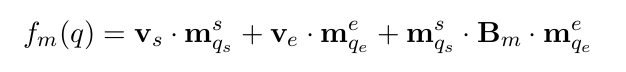
\includegraphics[width=0.7\textwidth]{Assets/Kirstain1}
    \caption{Bilinear function: start/end Mention embeddings: \textbf{m}\textsuperscript{s}, \textbf{m}\textsuperscript{e}}
    \label{fig:s2e1}
\end{figure}
The model computes \gls{coref_mention} scores as bi-affine products over the start and end \gls{token} representations (\textbf{m}\textsuperscript{s}, \textbf{m}\textsuperscript{e}) with
\textbf{v}\textsubscript{s}, \textbf{v}\textsubscript{e} and \textbf{B}\textsubscript{m} as trainable matrices (Fig.\ref{fig:s2e1}).
\begin{figure}[H]   %[h] puts picture right here. 't' stands for to, 'b' stands for bottom
    \centering
    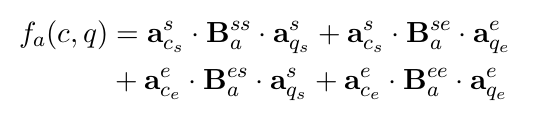
\includegraphics[width=0.6\textwidth]{Assets/Kirstain2}
    \caption{Bilinear function: start/end Antecedent embeddings:  \textbf{a}\textsuperscript{s}, \textbf{a}\textsuperscript{e}}
    \label{fig:s2e2}
\end{figure}
Similarly, it also extracts start and end \gls{token} representations (\textbf{a}\textsuperscript{s}, \textbf{a}\textsuperscript{e}) for
the antecedent scoring function with \textbf{B}\textsubscript{m} as another trainable matrix (Fig.\ref{fig:s2e2}).
This calculation is equivalent to computing a bilinear transformation between the concatenation of each \gls{span}’s boundary \glspl{token}’ representations,
but bypasses the need to create n\textsuperscript{2} explicit \gls{span} representations (for Bi-Gram \gls{span}) und thus reduces complexity \cite{KirstainCoref}.
The model is the fastest of all known \gls{coref_definition} models and, with an F1-score of 80.4, currently ranks fourth \cite{CorefEvaluation} in regard to prediction performance.

\paragraph{Available Models}
Based on these research papers, the following Python modules are available:

\subparagraph{AllenNLP}
AllenNLP \cite{AllenNLP} is an AI platform supported by the Allen Institute for Artificial Intelligence \cite{AllenAI}.
AllenNLP offers multiple pre-trained models and a pip-installable Python module \cite{AllenNLP}.
Among the models offered is a pre-trained \gls{coref_resolution_definition} model that is based on the c2f-model by Lee et al.\cite{CorefCoarseFine}.
The GloVe embeddings in the original paper \cite{CorefCoarseFine} have been substituted with \gls{SpanBERT} embeddings \cite{AllenNLPCorefModel}.
Unfortunately, since 2022 the AllenNLP ecosystem is in maintenance mode.
Dependencies to more recent Python versions are not upgraded and the most recent training for the \emph{coref-spanbert-large}-model goes back to March 2021.
Additionally, AllenNLP only offers pre-trained models for English but not for German.

\subparagraph{F-COREF}
F-COREF is a Python implementation and an adopted version of the s2e-model by Kirstain et al. \cite{KirstainCoref}.
F-COREF predicts \glspl{coref_cluster} 29 times faster than the AllenNLP model and requires only 15\% of its GPU memory use, with only a small
drop in performance (78.5 vs 79.6 average F1) \cite{FastCoref}.
Unfortunately, F-COREF currently only has a pre-trained model for English but not for German.

\subparagraph{Coreferee}
Coreferee \cite{Coreferee} is a pip-installable Python package that uses a mixture of \glspl{ann} and programmed language-specific rules.
It focuses heavily on detecting \glspl{anaphora} and noun phrases and thus depends on the grammatical and syntactical capabilities of spacy \cite{spacy}.
The likelihood scores for anaphoric pairs are calculated by utilizing the contextualized vectors of the underlying and pre-trained spacy models.
Specific language packages other than English exist for German, Polish and French and must be downloaded individually.

\subparagraph{Crosslingual-Coreference}\label{subpar:crosslingual-coreference}
The Crosslingual-Coreference model \cite{xxCoref} builds on the AllenNLP-Coreference model \cite{AllenNLPCorefModel} but modifies its \emph{coref\_resolved}-method.
It investigates all the \glspl{coref_cluster} found by the AllenNLP-Coreference model, but only considers \glspl{coref_cluster} that contain a noun phrase \cite{AllenCorefModelModification}.
To determine if a \gls{coref_cluster} contains a noun phrase, it uses the \gls{pos}-tagger of pre-trained models from spacy \cite{spacy} that are also available in languages other than English.
If the model parameter is set to \emph{minilm}, the \gls{llm} used in resolving \glspl{coref_cluster} is multilingual and pre-trained by Microsoft \cite{xxCorefMinilmModel}.
As such, this model can be applied multilingual, i.e. to English and German.

\paragraph{Evaluated Pre-Trained Models}
As only the Coreferee \cite{Coreferee} and Crosslingual-Coreference model \cite{xxCoref} are available for the German language, in the project only those two pre-trained models were evaluated against each other.
I tried both extensively with multiple texts, and the Crosslingual-Coreference model \cite{xxCoref} clearly outperformed the Coreferee \cite{Coreferee} model.
It found more \gls{coref_definition} mentions and had a lower entity confusion rate in texts that contained multiple entities.
The Crosslingual-Coreference model \cite{xxCoref} was later compared against a \gls{gen-llm} approach.

\subsection{\gls{gen-llm} Models}\label{subsec:generative-llm-models}
\paragraph{Pre-Trained AND Generative}\label{par:pretrained-and-gen-llm}
Besides using \glspl{gen-llm} and \gls{prompt} requests directly, there are also dedicated architectures and indirect ways to extract \glspl{coref_definition} from text.
In the previous section, the \gls{coref_definition} model by Google Research \cite{CorefSeq2Seq} was classified as a pre-trained model, but it could also be classified as a \gls{gen-llm} model as the boundaries between these two types are increasingly blurry.

The pre-trained Google model \cite{CorefSeq2Seq} is a sequence-to-sequence model that uses both stacks of the \gls{Transformer} architecture, i.e. the encoder \emph{and} the decoder.
It so generates new text based on an input sequence where the input sequence is an untagged string and the output sequence the input string plus tags attached to it.
The tags contain the desired \gls{coref_definition} annotations.
The model is trained with the aim to annotate the input string with the respective \gls{coref_definition} tags.

This approach is very similar to the one Wang et al \cite{gptner} use in their model for the \gls{ner} task (see \ref{subsec:deep-learning-models}).

Whereas the Google \cite{CorefSeq2Seq} model introduces some extra layers to an encoder-decoder stack, Zhang et al \cite{zhangcorefseq2seq} use a plain pre-trained encoder-decoder (text-to-text) T5 model \cite{googlet5} and finetune it in a supervised way with annotated examples.
The source sequence contains the input string and the target sequence the \emph{\gls{coref_definition}-annotated} input string.
During finetuning, the classification task uses the usual source-target sequence pair and tries to minimize the cross-entropy loss given the per-\gls{token} labels \cite{zhangcorefseq2seq}.
\paragraph{Models used}
As stated previously, neither the Google \cite{CorefSeq2Seq} model nor the Zhang et al \cite{zhangcorefseq2seq} model are (easily) available as a Python module.
I therefore tested the \gls{gen-llm} approach directly as described in the next section.

\section{Code Implementation}
\subsection{Implementation of Pre-Trained Model}
As stated previously (see Section \ref{subpar:crosslingual-coreference}), the Crosslingual-Coreference model \cite{xxCoref} is based on the deprecated AllenNLP-Coreference model \cite{AllenNLPCorefModel}, depends on the \gls{pos}-tagger from a certain spacy version and uses a fine-tuned and pre-trained Microsoft \gls{llm} that was last updated in 2021.
It has some issues for Python versions greater than 3.10 and dependency conflicts to other Python libraries in the project that could not be resolved.


I thus decided to run the Crosslingual-Coreference model \cite{xxCoref} in an isolated environment using Docker.
The files for building the Docker container can be found in the \emph{/src/D\_coref/img\_xx\_coref\_files} directory that also contains a Dockerfile and a requirements.txt file.
The Docker container is accessible by using http requests.

The Crosslingual-Coreference model \cite{xxCoref} in the Docker container is run as a spacy pipeline-component that attaches found \glspl{coref_cluster} to spacy's Doc-object custom extensions.
The \glspl{coref_cluster} are nested Python lists in the format
\begin{center}
\scriptsize\textbf{{[[[cl1\_start1, cl1\_end1], [cl1\_start2, cl1\_end2]], [[cl2\_start1, cl2\_end1], [cl2\_start2, cl2\_end2]]]}}
\end{center}
where character start and end index positions for each word in a \gls{coref_cluster} are shown.

The function \emph{spread\_comp\_ext\_to\_coref\_cluster\_spans()} in Python-Code \ref{code:spread-comp-ext-to-coref-cluster-spans}

\begin{listing}[H]
    \captionof{listing}{spread\_comp\_ext\_to\_coref\_cluster\_spans()}
    \inputminted[
    firstline=348,
    lastline=369,
    firstnumber=348,
    ]{python}{/media/rainergo/PROJECTS/UASFRA-MS-Thesis/src/B_spacy_pipeline/spacy_pipe_funcs.py}
    \label{code:spread-comp-ext-to-coref-cluster-spans}
\end{listing}
first checks if any \gls{coref_cluster} word overlaps with a spacy custom extension \gls{span} that has a company name and company symbol attached to it.
If this is the case, it creates a new instance of the SearchMatch class with the same company name and company symbol for every other member of the \gls{coref_cluster}.

Before setting the found \glspl{coref_definition} to the spacy custom extensions, the function \emph{resolve\_span\_conflicts\_and\_set\_new\_ents()} in Python-Code \ref{code:resolve-span-conflicts-and-set-new-ents}
\begin{listing}[H]
    \captionof{listing}{resolve\_span\_conflicts\_and\_set\_new\_ents()}
    \inputminted[
    firstline=92,
    lastline=127,
    firstnumber=92,
    ]{python}{/media/rainergo/PROJECTS/UASFRA-MS-Thesis/src/B_spacy_pipeline/spacy_pipe_funcs.py}
    \label{code:resolve-span-conflicts-and-set-new-ents}
\end{listing}

checks if the respective spacy \gls{token} or \gls{span} already has these extensions set by the previous \gls{ner} component of the pipeline.
Only if this is not the case, the custom extension is set with the information from the SearchMatch instances.

\subsection{Implementation of \gls{gen-llm} Model}\label{subsec:langchain-explain}
To implement the \gls{gen-llm} model directly as reasoned in Section \ref{par:pretrained-and-gen-llm}, the Python LangChain \cite{LangChain} library was used.
LangChain is a modular LLM framework where components such as \glspl{prompt}, \glspl{llm}, Agents and Tools can be chained together to build an \gls{llm} pipeline.

The latest LangChain version 0.3 uses Pydantic version 2 \cite{Pydantic}, a mandatory type checking library, that had unresolvable dependency conflicts with existing libraries in the project.
For this reason, I also isolated the \gls{gen-llm} approach by using Docker.
The files for building the Docker container can be found in the \emph{/src/D\_coref/img\_llm\_extract\_coref\_files} directory that, among other files, contains a Dockerfile and a requirements.txt file.

\paragraph{Data Model}\label{par:coref-data-model}
In the mentioned directory, there is also a Python file named \emph{data\_models.py} (see Python-Code \ref{code:data-model-coref-llm-extract}) that lays out the desired format of the \gls{llm} response and the format of messages in the \gls{prompt}.
This is important because \gls{gen-llm}s usually suffer to deliver the generated text response in an appropriate format such as JSON so that it can be further processed by an algorithm.

\begin{listing}[H]
    \captionof{listing}{Data Model Coref LLM Extract}
    \inputminted[
    firstline=4,
    lastline=36,
    firstnumber=4,
    ]{python}{/media/rainergo/PROJECTS/UASFRA-MS-Thesis/src/D_coref/img_llm_extract_coref_files/data_models.py}
    \label{code:data-model-coref-llm-extract}
\end{listing}

Python-Code \ref{code:data-model-coref-llm-extract} shows the data model which consists of four Python classes that all inherit from Pydantic's \emph{BaseModel}.
This way, Pydantic in the background checks instances of these classes for their type (such as Integer, Float, String, etc.) and raises an error if the value of the respective instance variable does not comply with it.

\subparagraph{\gls{prompt}}
The \gls{prompt} for the \gls{gen-llm} model contains examples (few-shots) in the form of instances of these Pydantic classes.
Instances of the class Cluster contain the article text, an instance of the class ClusterHead and potentially multiple instances of the class Coreference.

Instances of the ClusterHead class are created with the information that was previously extracted by the pipeline's \gls{ner} component: the company name (\emph{head\_text}) and the start (\emph{head\_index\_start}) and end (\emph{head\_index\_end}) position of this company name within the article text.

Instances of the class \gls{coref_definition} contain the \gls{coref_definition} string (\emph{coref\_text}) and the \gls{coref_definition} string with two words on the right and left (\emph{coref\_with\_surroundings}).


As an example, let's say that the article text is

\begin{center}
    \textbf{Siemens manufactures trains. It is located in Munich.}
\end{center}
then the according few-shot example in the \gls{prompt} would be

\begin{center}
\scriptsize\textbf{{
Cluster(cluster\_id=1, text="Siemens manufactures trains. It is located in Munich.",\newline
        cluster\_head=ClusterHead(head\_text="Siemens", head\_index\_start=0, head\_index\_end=7),\newline
        coreferences=[Coreference(coref\_text="It", coref\_with\_surroundings="manufactures trains. It is located")])}}
\end{center}

The question is why the \gls{coref_definition} class does not include position indexes of the found \gls{coref_definition} word within the text similar to the \emph{head\_index\_start} and \emph{head\_index\_end} variables for the company name.
Then the subsequent algorithm could easily locate the \gls{coref_definition} words in the text and attach them to the respective custom extensions of the Doc-object in the spacy pipeline.

I tried to force the \gls{gen-llm} to return those position integer values for \glspl{coref_definition} it found but the model, even equipped with the respective tools in the LangChain pipeline, did not succeed.
I assume that this could also be the reason why Wang et al \cite{gptner} had their \gls{ner} model generate string annotations instead of returning text position indexes such as

\begin{center}
    \emph{@@Columbus\#\# is a city}
\end{center}
for the input sequence \emph{Columbus is a city} (see Section \ref{par:gpt-ner}).

I also could have asked the \gls{gen-llm} to annotate the \gls{coref_definition} it found with the same symbols such as:
\begin{center}
    \textbf{Siemens manufactures trains. @@It\#\# is located in Munich.}
\end{center}

But the problem was that the article text, even after cleaning, already contained such symbols (i.e.\emph{@} and\emph{\#}) so that a subsequent algorithm could potentially have confused them.

The few-shot examples provided to the \gls{gen-llm} can be found in: \newline
\emph{src/D\_coref/img\_llm\_extract\_coref\_files/examples.py}

\subparagraph{Response Format}
The Pydantic classes are not only used for few-shot examples in the \gls{prompt}, but also for defining the response format.
The LangChain pipeline or chain is defined in \newline
\emph{src/D\_coref/img\_llm\_extract\_coref\_files/coref\_langchain.py}:

\begin{listing}[H]
    \captionof{listing}{LangChain pipeline for COREF}
    \inputminted[
    firstline=19,
    lastline=40,
    firstnumber=19,
    ]{python}{/media/rainergo/PROJECTS/UASFRA-MS-Thesis/src/D_coref/img_llm_extract_coref_files/coref_langchain.py}
    \label{code:langchain-coref}
\end{listing}

The LangChain chain is built in line 26 of the above code and connects a filled PromptTemplate with an \gls{llm} module, in this case OpenAI's ChatOpenAI module running their \textbf{gpt-4o} model.

In line 25, the ChatOpenAI module via the function
\begin{center}
\emph{with\_structured\_output(schema=Cluster)}
\end{center}
is bound to Pydantic's Cluster class, as discussed previously.
This forces the \gls{llm} to return its response in a format that is compliant with that class.
As the \gls{gen-llm} approach is run via a Docker container and http requests, the Pydantic class instances are converted to serializable Python dictionaries and \gls{json} and back to Pydantic class instances in the process.

\subparagraph{Processing the LLM Response}
Ideally, the response from the \gls{llm} is in the desired format and, among other information, contains the values for the variables \emph{coref\_text} and \emph{coref\_with\_surroundings}.
They will now be converted to values that can be attached as custom extensions in the Doc-object of the spacy pipeline by the following function:

\begin{listing}[H]
    \captionof{listing}{Convert LLM response to Matches}
    \inputminted[
    firstline=418,
    lastline=445,
    firstnumber=418,
    fontsize=\tiny,
    ]{python}{/media/rainergo/PROJECTS/UASFRA-MS-Thesis/src/B_spacy_pipeline/spacy_pipe_funcs.py}
    \label{code:llm-to-match}
\end{listing}

The \gls{coref_definition} position index within the text are determined by using \gls{Regex} functions and patterns.

First, the position indexes of the \emph{coref\_with\_surroundings} text within the article text, and afterward the \emph{coref\_text} within the \emph{coref\_with\_surroundings} text are determined.
A \gls{Regex} search for the \emph{coref\_text} in the article text \underline{alone} would not be sufficient,
because the \emph{coref\_text} could be a common word such as \emph{it}, which might occur multiple times in the text without being a \gls{coref_definition}.
The two required words to the left and right of the actual \gls{coref_definition} word ensure a text sequence of at least five \glspl{token} which is unlikely to occur twice in the given article text.

The process for each \gls{coref_definition} yields a Python \emph{re Match object} that contains the start and end index of the \emph{coref\_text} within the article text.

Before the information is attached to the \gls{token} or \gls{span} custom extensions of the Doc-object, the function \emph{resolve\_span\_conflicts\_and\_set\_new\_ents()} again checks if there is an overlap with custom extension values that were already set by the previous \gls{ner} pipeline component (see: Python-Code \ref{code:resolve-span-conflicts-and-set-new-ents}).

\subparagraph{Collecting Entities}
Once the spacy pipeline has run, the company information stored in the custom extensions, is collected.


It could be that a news article contains multiple sentences each mentioning multiple companies.
The functions
\begin{center}
    \emph{get\_ents\_with\_custom\_extension()} and \emph{get\_sentences\_with\_custom\_extensions()}
\end{center}
collect the company information fom the custom extensions in the spacy Doc-object and store them in a Python dictionary:

\begin{listing}[H]
    \captionof{listing}{Collection of custom extension information}
    \inputminted[
    firstline=49,
    lastline=63,
    firstnumber=49,
    fontsize=\tiny,
    ]{python}{/media/rainergo/PROJECTS/UASFRA-MS-Thesis/src/B_spacy_pipeline/spacy_pipe_funcs.py}
    \label{code:collect-entities}
\end{listing}

They make sure that multiple company mentions in a sentence are accounted for.
The resulting nested Python list of dictionaries is compiled for every article containing company information and structurally looks like this sample:

\begin{listing}[H]
    \captionof{listing}{Company information for article text}
    \inputminted[
    firstline=1,
    lastline=39,
    firstnumber=1,
    ]{python}{/media/rainergo/PROJECTS/UASFRA-MS-Thesis/doc/Assets/after_ner_coref.json}
    \label{code:dict-after-coref-and-ner}
\end{listing}

Sentences that contain more than one company mention within each dictionary store the information in another list of Python dictionaries.
For sentences that contain only one company mention, this list only contains one item.

\paragraph{Topic Sentences}\label{par:topic-sents}
The news articles are stored in a parquet file to be converted to a pandas DataFrame as described in Section \ref{ch:project_setup}.
Each row in the DataFrame contains one article and each list of Python dictionaries, as shown in the Python-Code \ref{code:dict-after-coref-and-ner}, is stored in one cell of the \emph{ner\_coref} column as object.\\

To do Topic Modelling on sentences as described in the next chapter, the nested list of Python dictionaries (Python-Code \ref{code:dict-after-coref-and-ner}) must be flattened first to have one sentence in each row of the DataFrame.
This is what the
\begin{center}
\emph{convert\_nested\_ner\_coref\_dict()}
\end{center}
function in the Python file \emph{main\_process.py} does:

\begin{listing}[H]
    \captionof{listing}{Un-Nesting \gls{ner} and COREF Information}
    \inputminted[
    firstline=78,
    lastline=84,
    firstnumber=78,
    ]{python}{/media/rainergo/PROJECTS/UASFRA-MS-Thesis/main_process.py}
    \label{code:unnest-dict-after-coref-and-ner}
\end{listing}

Before inserting new rows into the DataFrame, the function in line 80 inserts a new \emph{art\_id} column that is just the row index of the DataFrame.
As each row contains just one article, the new column preserves the article identification of the soon-to-be expanded DataFrame.
The pandas DataFrame function \emph{explode} in line 51 then creates new rows for each dictionary (shown in Python-Code \ref{code:dict-after-coref-and-ner})
and pandas \emph{string accessor} method in line 52 finally inserts the sentences into the new column \emph{top\_sent}.

\subsection{Comparing Pre-Trained vs. \gls{gen-llm} approach}
The \gls{gen-llm} approach outperforms the pre-trained Crosslingual-Coreference model \cite{xxCoref} on the sample text I tested them with.
The latter model performs well if the article text mentions only one company, but links \glspl{coref_definition} to the wrong company if multiple companies are mentioned.
Here, the pre-trained Crosslingual-Coreference model \cite{xxCoref} might show its lack for contextual understanding as the underlying \gls{llm} is only used for finding and resolving \glspl{coref_cluster} (see: Section \ref{subpar:crosslingual-coreference}).
The \gls{gen-llm} is not perfect either as it does not find all \glspl{coref_definition}, but those that are found are mostly correct.
In addition, the \gls{gen-llm} was only provided with four few-shot examples in the \gls{prompt} and adding more examples would probably improve the model further.
I thus have decided to use the \gls{gen-llm} approach for the task of \gls{coref_definition} resolution.

\subsection{Information Extraction Pipeline}
After the \gls{coref_resolution_definition} component has run, the spacy pipeline has attached the found company information to the respective custom extensions
that in a subsequent step will be stored as a list of dictionaries as shown in Python-Code \ref{code:dict-after-coref-and-ner}:
\begin{figure}[H]   %[h] puts picture right here. 't' stands for to, 'b' stands for bottom
    \centering
    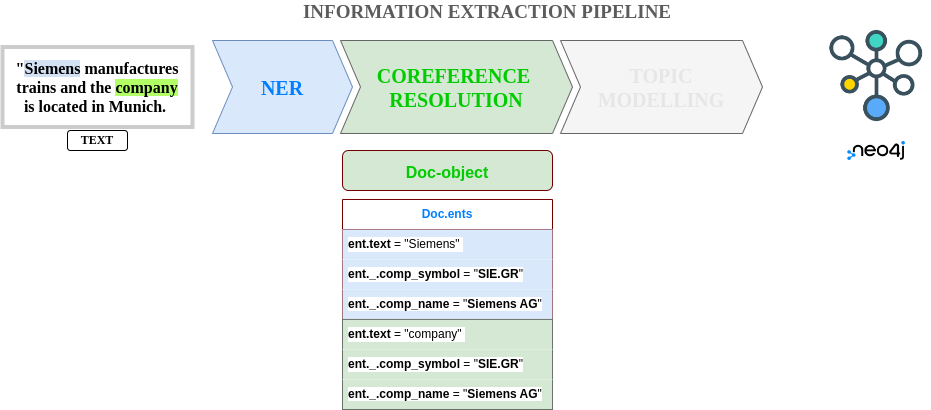
\includegraphics[width=0.85\textwidth]{Assets/pipelineCoref}
    \caption{spacy pipeline after COREF component}
    \label{fig:pipeCoref}
\end{figure}
In the example, it contains the company name \emph{Siemens} coming from the \gls{ner} component and the \gls{coref_definition} \emph{company} coming from the Coreference Resolution component.

















\chapter{Topic Modelling}\label{ch:topic-modelling}
\section{Information Extraction Types}

Information Extraction in \gls{nlp} can be subdivided into multiple fields \cite{iebook}, among them:

\begin{itemize}
    \item \textbf{Relation Extraction}: Extraction and classification of relations between named entities
    \item \textbf{Event Extraction}: Extraction of a temporal Event
    \item \textbf{Topic Modelling}: Assigment of a topic to a short text or document
\end{itemize}

The initial expectation for this project was to extract information from the article sentences in the form of triples:

\begin{center}
\textbf{Triple: Subject – Relation – Object}
\end{center}

where either the Subject or the Object would be a corporate entity (\gls{org}).

If the Subject were a company, the Object could either be another company or any other common named entity type from the set of \gls{org}, \gls{per} or \gls{loc}, and vice versa.

The assumption was that these Subjects and Objects would appear in the same sentence as in the following example:
\begin{figure}[H]
    \centering
    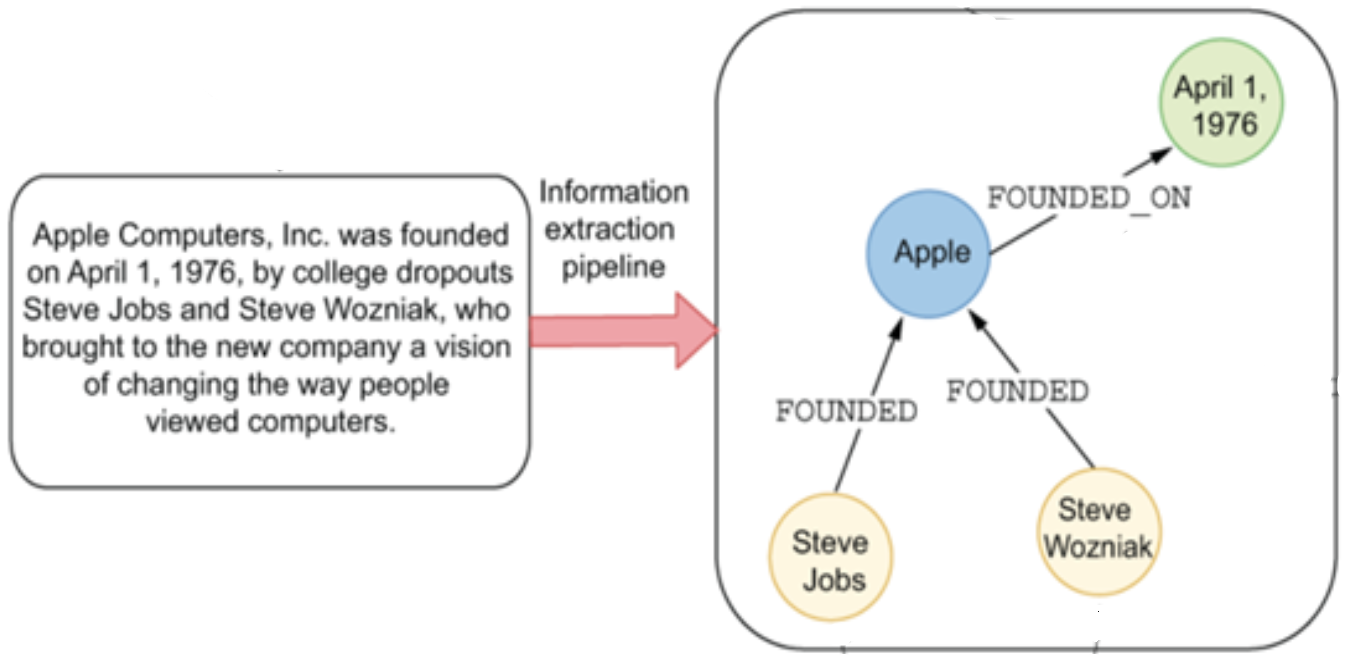
\includegraphics[width=1.0\textwidth]{Assets/sub-pred-obj}
    \caption{Triple: Subject: Person - Relation: Founded - Object: Apple}
    \label{fig:triples}
\end{figure}

After investigation of the news articles, it became clear that the limitation to only extract Relation triples was too restrictive.
Many article sentences only contained one common named entity type or described an Event rather than a relationship between entities.

In some other sentences, Subjects or Objects could have been assigned to a wider and less common set of entity types such as \emph{Product}, \emph{Money} or \emph{Law},
but this would have required to enlarge the set with many new custom entity types to cover the most fundamental themes in the finance domain.

It would also have meant to increase the complexity of the Knowledge Graph and deviate from the goal of the project, which was
to extract information from news articles with a focus on particular companies.
To answer the central question
\begin{center}
    \textbf{What is the company news all about?}
\end{center}
a more general and more comprehensive extraction type was needed.


Topic Modelling can be done on the sentence level and does not require entity pairs.
Topics can cover Events as well as Relations between entities and a wide array of finance themes.
Extracting information via Topic Modelling thus seems more appropriate for the data and task given than Relation Extraction.

\section{Traditional Topic Modelling}\label{sec:traditional_approaches}
Most of the traditional Topic Modelling methods are based on absolute (Bag-of-Word: Section \ref{subsec:bag-of-words}) or relative (TF-IDF: Section \ref{subsec:tf-idf}) word counts as discussed in Section \ref{ch:text-representation}.

They also return topics in the form of most frequent words where the user must first read the words per topic to get a sense of what the topic is all about, see Figure \ref{fig:lda-out}.

\begin{figure}[H]   %[h] puts picture right here. 't' stands for to, 'b' stands for bottom
    \centering
    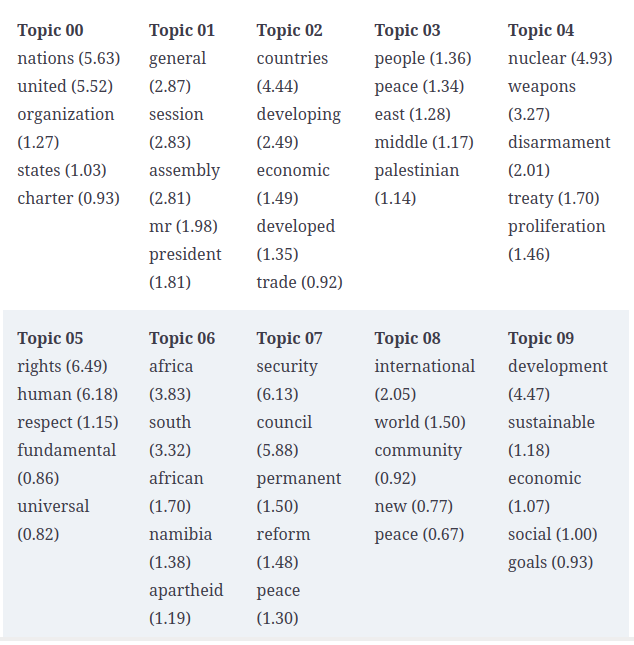
\includegraphics[width=0.60\textwidth]{Assets/lda-out}
    \caption{10 Topics and their most frequent words. Source: \cite{blueprints}}
    \label{fig:lda-out}
\end{figure}

\subsection{\gls{nmf}}\label{subsec:nmf}
In the Non-Negative Matrix Factorization method (\gls{nmf}), the most frequent words are retrieved by doing a
matrix decomposition of the \gls{document_term_matrix} (see Section \ref{fig:document_term_matrix}) which in the following Figure is dubbed \emph{Documents-Words Matrix}:

\begin{figure}[H]   %[h] puts picture right here. 't' stands for to, 'b' stands for bottom
    \centering
    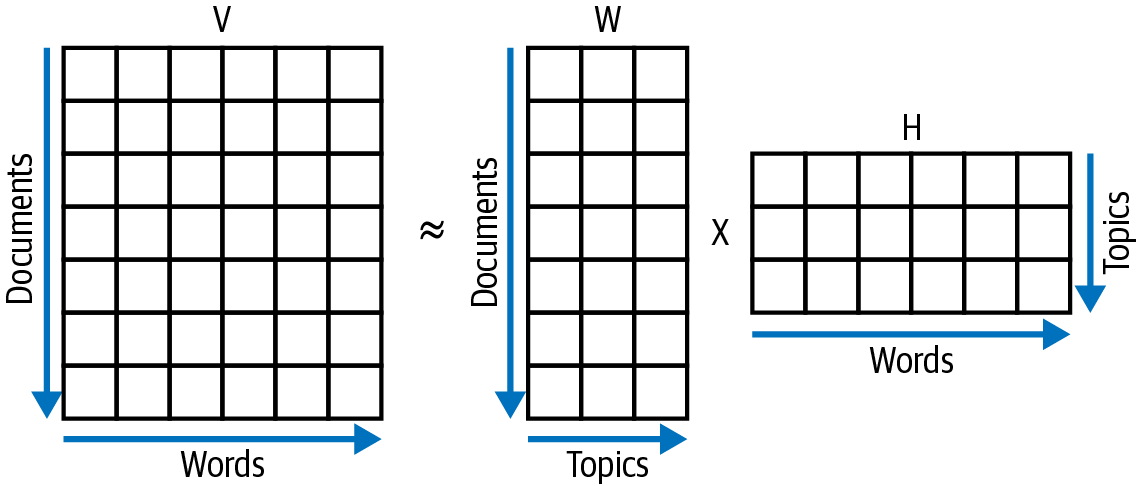
\includegraphics[width=0.70\textwidth]{Assets/nmf}
    \caption{\gls{nmf}: Source: \cite{blueprints}}
    \label{fig:nmf}
\end{figure}

The Documents-Topics matrix in the middle of Figure \ref{fig:nmf} maps Documents to Topics whereas the Words-Topics matrix on the right maps topics to their features, i.e. the words in the \gls{vocabulary}.
In most implementations, a rank parameter (or \emph{n\_components} parameter in Scikit-Learn's implementation \cite{nmf-implementation}) can be provided so that the word dimension of the \gls{document_term_matrix} first gets reduced before it is decomposed.
Because of this, \gls{nmf} can also be used as a dimension reduction method \cite{nmf-implementation}.
To get the most frequent words, each row in the Words-Topics matrix is sorted by its highest values with their respective column indexes being looked up in the \gls{vocabulary}.
The number of topics can be chosen arbitrarily but a smaller number will "throw" more words into one topic which makes the decomposition less exact \cite{blueprints}.

\subsection{\gls{svd}}\label{subsec:svd}
A very similar method is the Singular Value Decomposition (\gls{svd}) that decomposes the \gls{document_term_matrix} into three matrices:

\begin{figure}[H]   %[h] puts picture right here. 't' stands for to, 'b' stands for bottom
    \centering
    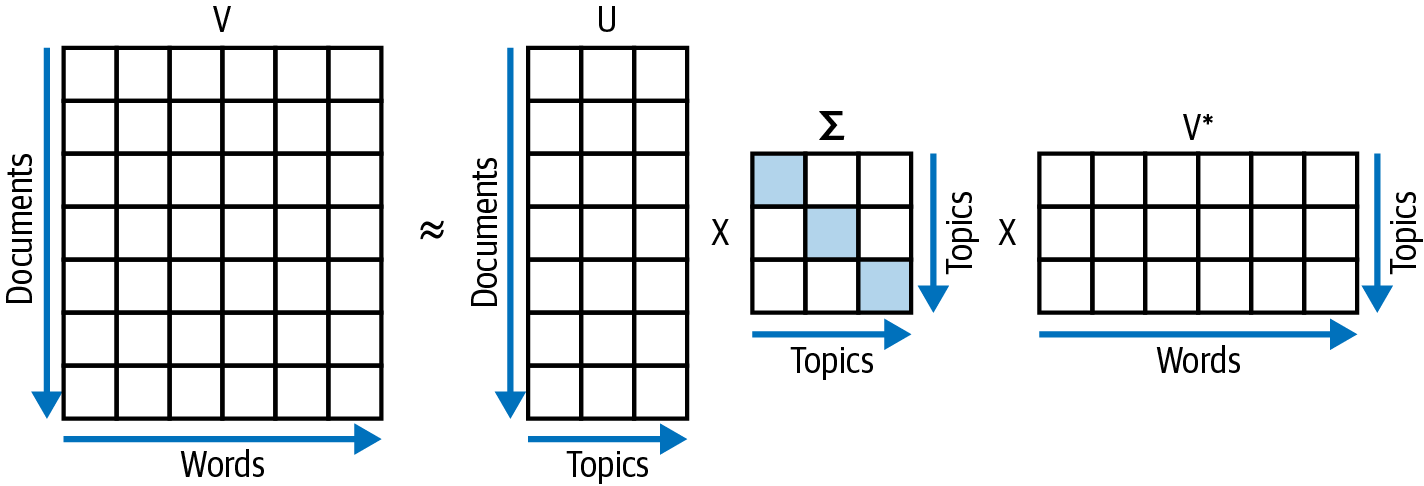
\includegraphics[width=0.70\textwidth]{Assets/svd}
    \caption{\gls{svd}: Source: \cite{blueprints}}
    \label{fig:svd}
\end{figure}

The nice thing about the \gls{svd} is that the quadratic Topics-Topics matrix (third matrix from left in Figure \ref{fig:svd}) on its diagonal contains the singular values which express the importance of each topic in a document.
A higher singular value indicates a topic that captures more of the variance (or information) in the corpus \cite{blueprints}.
From the most right Words-Topic matrix, the most important words per topic again can be extracted as described above (Section \ref{subsec:nmf}).

\subsection{\gls{lda}}\label{subsec:lda}
Latent Dirichlet Allocation (\gls{lda}), before the arrival of \glspl{llm}, had been the most prominent method for Topic Modelling \cite{blueprints}.
\gls{lda}, contrary to the previous methods above, is a probabilistic method that is based on the assumption that each Document contains a mix of a few different topics.
The method starts by randomly allocating words to each topic and also allocating topics to each document according to a Dirichlet distribution (\emph{Dirichlet prior}) \cite{blueprints}.
It then tries to re-create the words from the original document with stochastic sampling.
At the end of the optimization process, LDA also returns topics as a list of most frequent words as the \gls{nmf} and \gls{lda} methods do, but with a different distribution.

\section{Embedding-based Topic Modelling}\label{sec:topic_embedding_approaches}
As with most other fields in \gls{nlp}, the advent of \glspl{llm} also changed the way Topic Modelling can be approached today.
As the input data or features of traditional Topic Models are static words, they do to not take into account
the word's changing contextual meaning in different sentences, as already discussed in Section \ref{sec:word-embeddings}.
Thus, it is no wonder that today's best performing Topic Models are all embedding-based \cite{leaderboard-topic-models}.


\glspl{llm} can be used for Topic Modelling either with Pre-Trained or with \gls{gen-llm}s.

\subsection{Pre-Trained Topic Models}
Topic Modelling can be considered a classical text classification task and there are many pre-trained, publicly available models on HuggingFace \cite{huggingface} (see Figure \ref{fig:huggingface-topic-models}) or other platforms, even for multilingual text.

\begin{figure}[H]   %[h] puts picture right here. 't' stands for to, 'b' stands for bottom
    \centering
    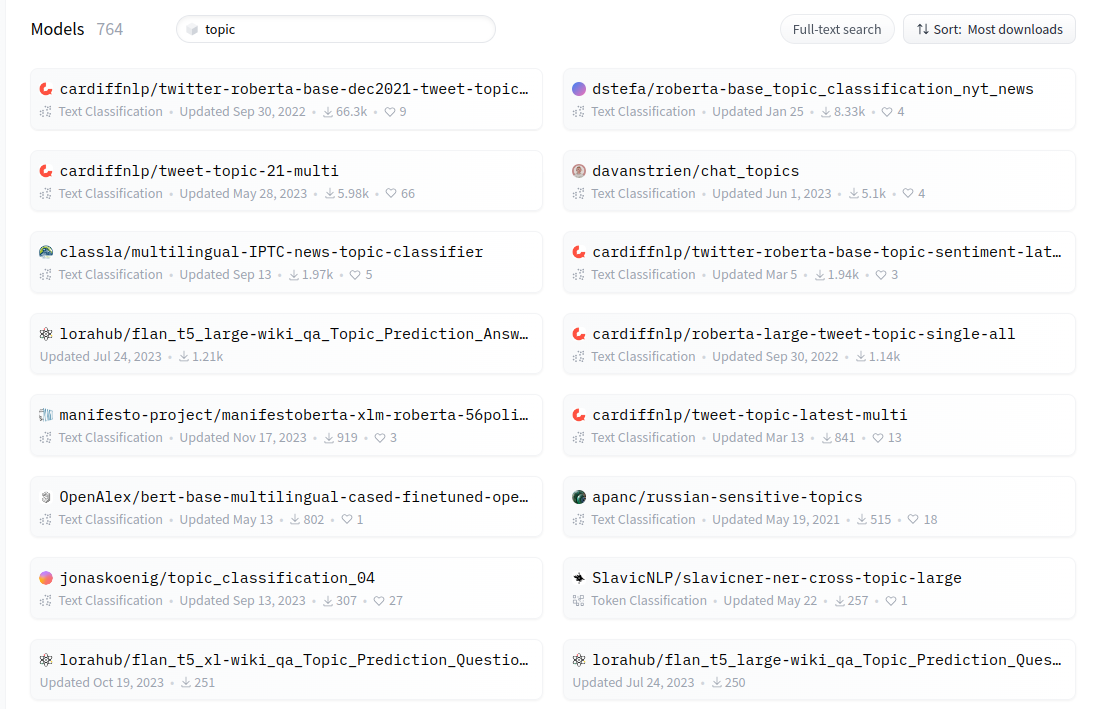
\includegraphics[width=0.85\textwidth]{Assets/huggingface-topic-models}
    \caption{Hugging Face Topic Models. Source: \cite{huggingface}}
    \label{fig:huggingface-topic-models}
\end{figure}

Unfortunately, the pre-trained Topic Models on Hugging Face \cite{huggingface} are either trained on labels that are very broadly categorized (see Figure \ref{fig:huggingface-topic-labels}) or very tightly confined to a narrow domain or language.

\begin{figure}[H]
\centering
\begin{minipage}{.35\linewidth}
  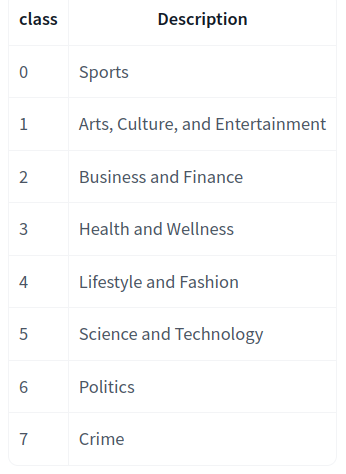
\includegraphics[width=\linewidth]{Assets/topic-classes-1}
  \label{img1}
\end{minipage}
\hspace{.05\linewidth}
\begin{minipage}{.55\linewidth}
  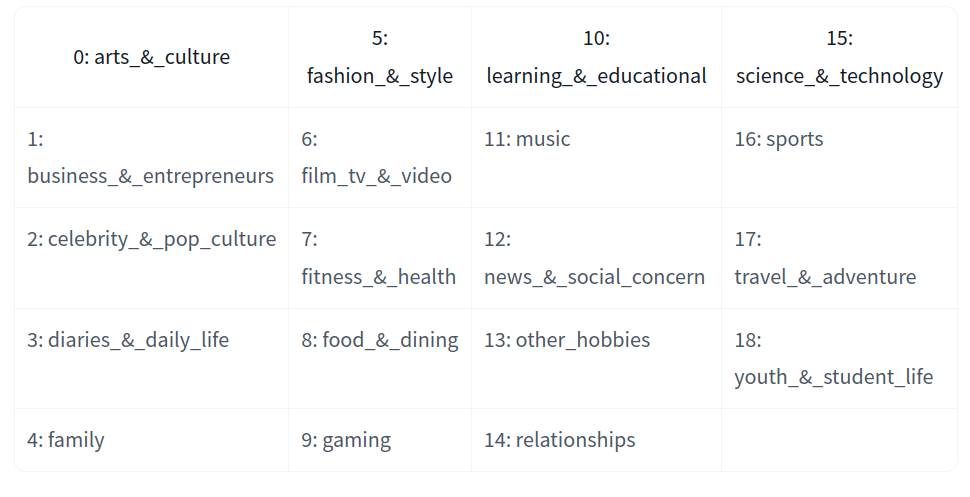
\includegraphics[width=\linewidth]{Assets/topic-classes-2}
  \label{img2}
\end{minipage}
    \captionof{figure}{Hugging Face Topic Models - Typical labels. Sources: \cite{topic-cardiffnlp}\cite{topic-stefanidis}}
    \label{fig:huggingface-topic-labels}
\end{figure}

After extensively researching the domains of these models, I conclude that none of them fits the corporate financial news domain and the given data very well.

It could be possible to fine-tune a model and I would expect the performance of such models to be quite good.
But fine-tuning would require to label and compile a lot of training samples which would go beyond the scope of this thesis.

\subsection{BERTopic}\label{subsec:bertopic}
Another kind of pre-trained model is BERTopic \cite{bertopic}.
BERTopic is similar to traditional models in that it returns a most-common-word list per topic for which the user must define a topic label manually.
But it differs from traditional models in that it does not use word vectors but Sentence Transformer (or SBERT) \cite{sentence-bert} embeddings.
BERTopic further uses dimension reduction and clustering techniques. \\
SBERT is a modification of the pre-trained \gls{BERT} model that uses siamese and triplet network structures to derive semantically meaningful sentence embeddings that can be compared using cosine-similarity.
This reduces the effort for finding the most similar pair of sentences significantly, while maintaining the accuracy from BERT \cite{sentence-bert}. \\


BERTopic \cite{bertopic} is a modular system in the sense that individual components can be substituted depending on the dataset and use case.
The modules and main steps to compose BERTopic \cite{bertopic} are:

\begin{enumerate}
    \item \textbf{Embeddings}: Choose and apply an embedding component, typically SBERT \cite{sentence-bert}
    \item \textbf{Dimension Reduction}: Choose and apply a dimension reduction method on the embeddings
    \item \textbf{Clustering}: Choose and apply a clustering algorithm on the dimension-reduced embeddings
    \item \textbf{Aggregate Text}: Aggregate the text of all documents within each cluster
    \item \textbf{Apply \gls{tfidf} Vectorization}:  Apply \gls{tfidf} vectorization to each of the per-Cluster-aggregated texts \footnote{In BERTopic, this is called class-based \gls{tfidf} or \emph{c-TF-IDF}}
    \item \textbf{Most Frequent Words}: Get the most frequent words for each cluster according to \gls{tfidf}
\end{enumerate}

This approach ensures that the distinction of Topic Clusters is made on the basis of contextual embeddings (Step 1).
But it also ensures, that the Topic that each Cluster represents, can also be presented as a collection of its most frequent words (Step 4 and 5).

BERTopic \cite{bertopic} can be downloaded and is pip-installable.
Most of the components in BERTopic are built with existing libraries such as Scikit-Learn.
I also wanted to compare it with traditional Topic modelling approaches, so I decided to implement it myself.
In this proprietary implementation not only word embeddings can be used, but also traditional word vectors such as those used in a classic Bag-of-Word (Sec.\ref{subsec:bag-of-words}) or \gls{tfidf} (Sec.\ref{subsec:tf-idf}) approach.\\

The modules for the self-implemented models can be found in the
\begin{center}
\emph{src/E\_topic\_model/traditional}
\end{center}
directory.
The model follows the modularity and architecture of BERTopic in that the steps to build the model are similar:

\begin{enumerate}
    \item \textbf{topic\_prepare}: If desired, preprocesses the text to reduce the dimension of the \gls{vocabulary} as described in Section \ref{subsec:techniques-to-reduce-vocabulary}.
    \item \textbf{topic\_vectorize}: Choose between \gls{tfidf} (Sec.\ref{subsec:tf-idf}), Bag-of-Word (Sec.\ref{subsec:bag-of-words}), One-Hot (Sec.\ref{subsec:one-hot-encoding}) vectorization or Sentence Transformers embeddings
    \item \textbf{topic\_dim\_reduce}: Choose between multiple dimension reduction methods such as PCA, \gls{nmf}, UMAP, etc.
    \item \textbf{topic\_cluster}: Choose between multiple cluster methods such as HDBSCAN, KMEANS, MEANSHIFT, etc.
    \item \textbf{topic\_model}: Run all of the above components and calculate Topics by presenting the most frequent words of each Cluster
    \item \textbf{topic\_visualize}: Reduce the dimension of the word vectors or embeddings to three and display the data and Clusters in a Plotly Scatter-3d-Graph.
\end{enumerate}

In the same directory, there are two Jupyter notebooks that can be used for model training and prediction:
\emph{topic\_model\_train.ipynb} and \emph{topic\_model\_test.ipynb}.

The Jupyter Notebook \emph{topic\_model\_train.ipynb} was used to extensively test different combinations of text processing approaches, vectorization methods and
cluster algorithms, but the results were disappointing.

\paragraph{Sentence Transformer Embeddings}
When using the Sentence Transformer embedding method as BERTopic does by default, the Cluster algorithms all had difficulties in separating the data points, not
only visually (see Figure \ref{fig:topic-embedd-cluster}), but also by separating semantically coherent words and sentences into different Clusters.

\begin{figure}[H]   %[h] puts picture right here. 't' stands for to, 'b' stands for bottom
    \centering
    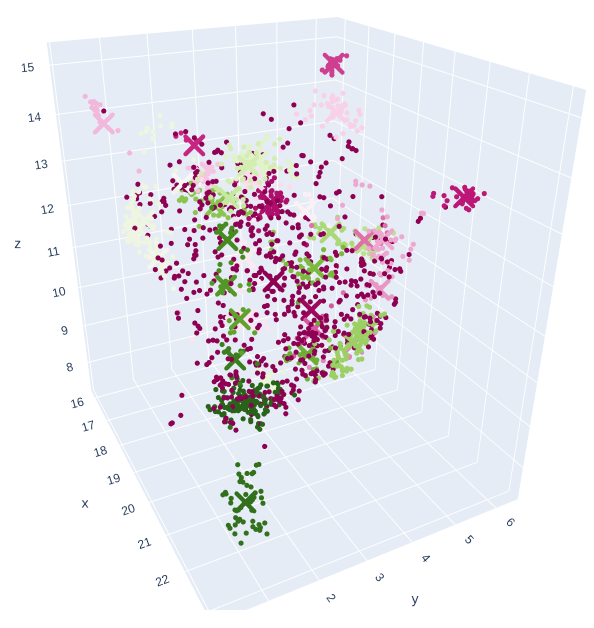
\includegraphics[width=0.50\textwidth]{Assets/topic-embedd-cluster}
    \caption{SBERT/Sentence Transformer embedding Cluster}
    \label{fig:topic-embedd-cluster}
\end{figure}

In Figure \ref{fig:topic-embedd-cluster}, UMAP was used to reduce the dimension to 20 and HDBSCAN was used to find clusters.
Although there are some clusters that are clearly separate from others, most of the clusters are within a close distance and the
separation of datapoints changes quickly with slightly different model parameters.
The same words appear in many clusters and manually looking at some individual sentences leads to the conclusion that sentences within clusters are not coherent.
The results were similar for other combinations of dimension reduction and clustering algorithms.

\paragraph{Word Vectors}
Looking at models were word vectors instead of embeddings were used, the performance of these models is not better:
\begin{figure}[H]   %[h] puts picture right here. 't' stands for to, 'b' stands for bottom
    \centering
    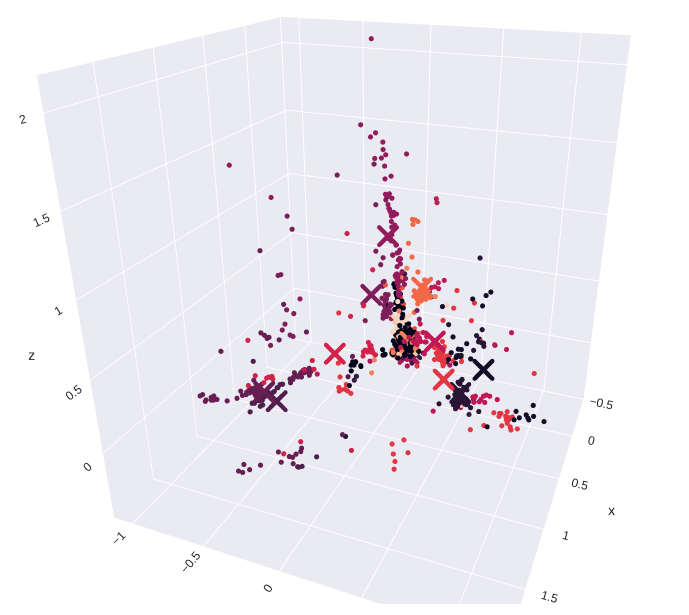
\includegraphics[width=0.50\textwidth]{Assets/topic-tfidf-cluster}
    \caption{TF-IDF Cluster}
    \label{fig:topic-tfidf-cluster}
\end{figure}

In Figure \ref{fig:topic-tfidf-cluster}, \gls{tfidf} was used for vectorization, PCA for dimension reduction and KMEANS for clustering.
The models suffer from the same shortcomings as the embedding based model above: same words appear in many clusters and sentences within clusters are not coherent.

\paragraph{Performance}
Although the financial news domain spreads across a wide range of topics, these topics are very nuanced and all have to do with company news.
I attribute the performance problems of the above methods to the fact that the differences between the individual sentences expressed
as distances in vector space are probably too small to extract meaningful clusters.

\section{Topic Modelling with \gls{gen-llm}s}\label{sec:topic-gen-llm}
Similar to creating a \gls{gen-llm} model for \gls{coref_resolution_definition}, the \gls{gen-llm} for Topic Modelling was also created with LangChain \cite{LangChain}.
As the problem of unresolvable dependency conflicts with existing Python libraries prevailed, the approach was again isolated with Docker.
The files for building the Docker container can be found in the
\begin{center}
\emph{/src/E\_topic\_model/img\_llm\_extract\_topics}
\end{center}
directory.

\paragraph{Data Model}
The \emph{data\_models.py} file in this directory contains the Python Enum \emph{TopicExplain} with the desired topic classes and a short description of each topic:

\begin{listing}[H]
    \captionof{listing}{Topic Model: Pre-Defined topics}
    \inputminted[
    firstline=9,
    lastline=29,
    firstnumber=9,
    fontsize=\tiny,
    ]{python}{/media/rainergo/PROJECTS/UASFRA-MS-Thesis/src/E_topic_model/img_llm_extract_topic/data_models.py}
    \label{code:llm-extract-topic-classes}
\end{listing}

There are 17 pre-defined topics formulated in German that were manually crafted by reading some of the article's sentences.
\emph{topic16} is dedicated to sentences that are incomplete and \emph{topic17} to all topics that are not covered by the previous 16 topics.\\

The process of defining topics could be facilitated by letting an \gls{llm} classify a set of sample sentences into an arbitrary number of topics, summarize each topic and express its overarching theme in a short sentence.
If manually crafted though, for a production use case, a more thorough semantic analysis of the article sentences and a re-assessment over the number of topics was also necessary.\\

The directory also contains a \emph{topics.py} file that provides sample sentences for each topic which are later used in the \gls{prompt} as few-shot examples.
Some of these few-shot examples are shown in Python-Code \ref{code:topic-examples}:

\begin{listing}[H]
    \captionof{listing}{Topic Model: Few Shot Examples}
    \inputminted[
    firstline=80,
    lastline=89,
    firstnumber=80,
    ]{python}{/media/rainergo/PROJECTS/UASFRA-MS-Thesis/src/E_topic_model/img_llm_extract_topic/topics.py}
    \label{code:topic-examples}
\end{listing}

As the few-shot examples often contain concrete company names, these company names therein were replaced by a \emph{Comp@Name@Placeholder} mask to avoid that the \gls{gen-llm} tries to match the company name of the sample sentence.\\

\paragraph{LangChain Code}
The LangChain code used in the Docker container is laid out in the \emph{topic\_langchain.py} file of the same directory, see Python-Code \ref{code:topic-langchain}:

\begin{listing}[H]
    \captionof{listing}{LangChain Topic Model}
    \inputminted[
    firstline=20,
    lastline=40,
    firstnumber=20,
    ]{python}{/media/rainergo/PROJECTS/UASFRA-MS-Thesis/src/E_topic_model/img_llm_extract_topic/topic_langchain.py}
    \label{code:topic-langchain}
\end{listing}
In line 26, the chain is built by \emph{piping} or connecting LangChain's \gls{prompt} component with the \gls{llm} component.
The \gls{prompt} contains the previously discussed few-shot \emph{examples} (line 27) compiled and organized by a Python function into an appropriate format.
It also contains the topics and their short descriptions (line 28) coming from the Python Enum \emph{TopicExplain} discussed above.\\

The sentences to be topic-classified are inserted into the \gls{prompt} (line 40) via an instance of a Python \emph{Frame} class (see Python-Code \ref{code:llm-extract-frame-class}) that inherits from Pydantic's BaseClass \cite{Pydantic}.
The same class in line 25 is also used in LangChain's \emph{ChatOpenAI} module function
\begin{center}
    \emph{llm.with\_structured\_output(schema=Frame)}
\end{center}
to force the \gls{llm} to return its response in the format of this class, as explained in Section \ref{par:coref-data-model}.

\begin{listing}[H]
    \captionof{listing}{Frame: A Pydantic BaseModel class}
    \inputminted[
    firstline=53,
    lastline=57,
    firstnumber=53,
    ]{python}{/media/rainergo/PROJECTS/UASFRA-MS-Thesis/src/E_topic_model/img_llm_extract_topic/data_models.py}
    \label{code:llm-extract-frame-class}
\end{listing}

\paragraph{Aggregation of Sentences}
The \emph{Frame} class, as the name implies, shall carry the data of a pandas DataFrame, namely the row \emph{indexes} of the DataFrame, the name of the column that contains the \emph{sentences} to be topic-classified and the \emph{topics} classes of those sentences to be returned by the \gls{gen-llm}.
The sentences to be classified are aggregated within a pandas DataFrame because the few-shot examples baked into the \gls{prompt} are rather long.
It would be very costly if the \gls{prompt} with its long few-shot examples would be sent for each sentence individually and separately.

\paragraph{The Token Limit Problem}
If there are many and long sentences to be topic-classified, the token limit that all \gls{gen-llm}s have imposed, will be reached.
To avoid that, the pandas DataFrame, later to be converted to a \emph{Frame} instance, first must be split into chunks.\\

This is what the function
\begin{center}
\emph{get\_topics\_from\_gen\_llm()} (Python-Code \ref{code:get-top-from-gen-llm})
\end{center}
in the \emph{main\_process.py} file will do.

\begin{listing}[H]
    \captionof{listing}{Frame: A Pydantic BaseModel class}
    \inputminted[
    firstline=124,
    lastline=157,
    firstnumber=124,
    ]{python}{/media/rainergo/PROJECTS/UASFRA-MS-Thesis/main_process.py}
    \label{code:get-top-from-gen-llm}
\end{listing}
It first chunks the passed DataFrame into a default size of 30 rows (line 130), converts it to a \emph{Frame} instance (line 131) and sends
the JSON-ized instance to the Docker container waiting for requests (line 133).
The LangChain model, as described above, in the Docker container forwards the Examples- and Topic-enhanced \gls{prompt} request to an OpenAI server and returns
the response from there, ideally in JSON-format (that complies with the \emph{Frame} class format), in line 140.

If the procedure succeeds, the topic classification of the \gls{gen-llm} for each DataFrame chunk first gets appended to a Python list that later will be used to create a new \emph{topics} column in the DataFrame.
If the procedure fails, it is tried once again and the request is resend.
If the procedure still fails, \emph{topic17} as the default spare class will be appended to the Python list in line 152.

The function returns the pandas DataFrame with an extra \emph{topics} column that contain one of the 17 Enum topics for each sentence.

\subsection{Comparing Pre-Trained vs. \gls{gen-llm} approach}
As outlined above, the cluster based methods such as the self-implemented BERTopic model, did not perform well on the Topic Modelling task.
In addition, they require to manually formulate a topic based on the most frequent words of a cluster.

The \gls{gen-llm} on the other side did perform well on the sentences I tested it with.
Most of the sentences were classified correctly.
For sentences that were expected to be classified differently, the actual and expected topic classes and examples were ambiguous and probably need some refinement.

I attribute the good performance of the \gls{gen-llm} to the power of a really large \gls{llm} (such as OpenAI's 4o model) that has the capacity to understand and distinguish even the most nuanced context.

I would expect a pre-trained \gls{llm}, such as those available on HuggingFace, to perform equally well after fine-tuning it with domain-specific topic labels and training data.

But as I did not go through the extensive process to compile and label such training data, in the project the \gls{gen-llm} was used for Topic Modelling.

\section{Information Extraction Pipeline}
After the Topic Modelling component has run, the \gls{gen-llm} has filled the pandas DataFrame column \emph{topics} in respect to each sentence in the column \emph{top\_sent}:
\begin{figure}[H]   %[h] puts picture right here. 't' stands for to, 'b' stands for bottom
    \centering
    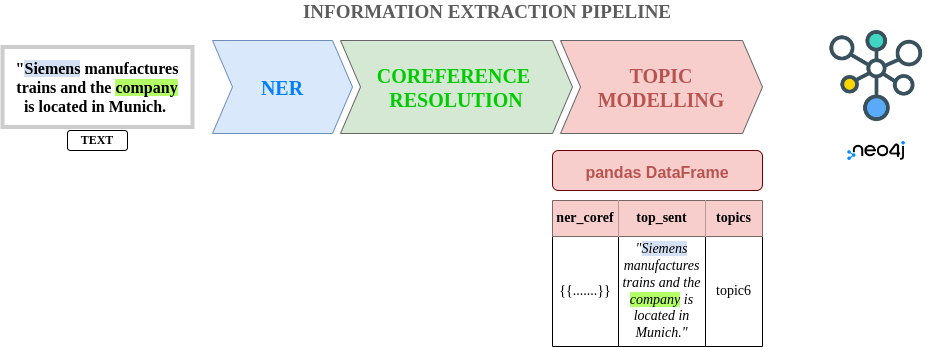
\includegraphics[width=0.90\textwidth]{Assets/pipelineTopic}
    \caption{DataFrame after Topic component}
    \label{fig:pipeTopic}
\end{figure}
In the example above, the DataFrame contains all the information coming from the \gls{ner} and \gls{coref_definition} components and one of the 17 possible topics for each sentence in which a company was found.



\chapter{Knowledge Graph\protect\footnote{Part of the Python code for this section was adopted from \cite{projdigi}}}\label{ch:knowledge_graph}
\section{Introduction}
As outlined in Chapter \ref{ch:introduction}, the goal of this project was to extract structured information from unstructured text and store this information in a Knowledge Graph.
A Knowledge Graph is an organized representation of real-world entities and their relationships which is typically stored in a graph database such as neo4j \cite{neo4j-kgdefinition}.
A graph database stores data as \emph{Nodes}, \emph{Relationships} and \emph{Properties} in a graph-like \cite{graph-definition} structure instead of in tables or documents \cite{neo4j}.
This enables the database to traverse \emph{Nodes} and \emph{Relationships} more quickly than relational databases, that would use computationally expensive \emph{JOIN} operations to retrieve inter-related information \cite{neo4j-kgdefinition}.

All the files for this chapter can be found in the \emph{src/F\_knowledge\_graph} directory.

\section{Knowledge Graph Creation}
A Knowledge Graph is defined by an \emph{Organizing Principle} \cite{neo4j-kgdefinition} or a \emph{Schema}.
The schema of the Knowledge Graph in this project is depicted in Figure \ref{fig:kg-schema-2}.
\begin{figure}[H]
	\centering
	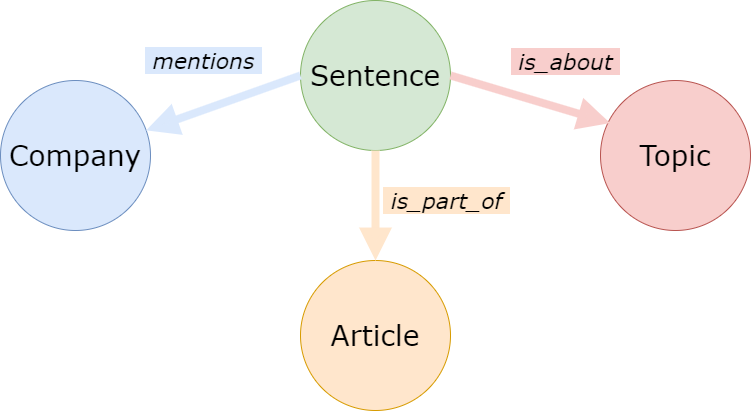
\includegraphics[width=0.75\textwidth]{Assets/kg_schema}
	\caption{Knowledge Graph Schema}
	\label{fig:kg-schema-2}
\end{figure}
The schema contains four Nodes (\emph{Article}, \emph{Sentence}, \emph{Company}, \emph{Topic}) and
three relationships (\emph{mentions}, \emph{is\_part\_of}, \emph{is\_about}), as described in Section \ref{ch:introduction}.

\paragraph{Ontology}
A Knowledge Graph \emph{Schema} can be outlined in different ways, for instance by using an \emph{Ontology}.
An \emph{Ontology} uses a modelling language to formally specify the concepts and relationships in a human- and machine-understandable way \cite{neo4j-kgdefinition}.

The most widely used ontology modelling languages are OWL (\emph{Web Ontology Language}) \cite{owl} and RDFS (\emph{Resource Description Framework Schema}) \cite{rdfs}.
Their most fundamental construct is a triple \cite{triples} consisting of
\begin{center}
\textbf{Subject - Predicate - Object}
\end{center}
tuples.
Multiple triples can be composed into a graph structure because objects can be subjects and vice versa and both can be connected via predicate relationships.\\
The textual presentation of the Ontology in this project is done with a Turtle \cite{turtle} file (suffix: \emph{.ttl}), a common data serialization format for storing triples.
The \emph{NewsArticles.ttl} Ontology file (Python-Code \ref{code:onto1}-\ref{code:onto3}) was created with Protege \cite{protege}, an open-source ontology editor by Stanford University.

\begin{listing}[H]
    \captionof{listing}{NewsArticles.ttl - Prefixes}
    \inputminted[
    firstline=1,
    lastline=8,
    firstnumber=1,
    ]{python}{/media/rainergo/PROJECTS/UASFRA-MS-Thesis/src/F_knowledge_graph/Ontologies/NewsArticles.ttl}
    \label{code:onto1}
\end{listing}

Turtle files usually start with prefixes that refer to other Ontology namespaces \cite{owl-guide} and their vocabulary \cite{owl-guide}.

In line 8 of the \emph{NewsArticles.ttl} file, the triple
\begin{center}
    \emph{subject}  ~~~~~~~~~~    \emph{predicate}  ~~~~~~~~~~  \emph{object}\\
    \textbf{rainergo: ~~~~~ rdf:type ~~~~~ owl:Ontology}
\end{center}
states that the prefix \emph{rainergo} in line 1 is of type \emph{Ontology} where \emph{type} and \emph{Ontology} themselves
are defined in triples that are accessible through their public \glspl{iri} in lines 2 and 3.

\begin{listing}[H]
    \captionof{listing}{NewsArticles.ttl - Classes or Nodes}
    \inputminted[
    firstline=87,
    lastline=101,
    firstnumber=87,
    ]{python}{/media/rainergo/PROJECTS/UASFRA-MS-Thesis/src/F_knowledge_graph/Ontologies/NewsArticles.ttl}
    \label{code:onto2}
\end{listing}

In lines 87 to 101, the classes or Nodes of the Knowledge Graph schema are defined, again with triples.

\begin{listing}[H]
    \captionof{listing}{NewsArticles.ttl - Relationships}
    \inputminted[
    firstline=10,
    lastline=27,
    firstnumber=10,
    ]{python}{/media/rainergo/PROJECTS/UASFRA-MS-Thesis/src/F_knowledge_graph/Ontologies/NewsArticles.ttl}
    \label{code:onto3}
\end{listing}

In lines 10 to 27, the relationships are defined with three triples for each relationship
where the second (predicate: \emph{domain}) and third (predicate: \emph{range}) triple represent its source and target Node.

\begin{listing}[H]
    \captionof{listing}{NewsArticles.ttl - Properties}
    \inputminted[
    firstline=29,
    lastline=50,
    firstnumber=29,
    ]{python}{/media/rainergo/PROJECTS/UASFRA-MS-Thesis/src/F_knowledge_graph/Ontologies/NewsArticles.ttl}
    \label{code:onto4}
\end{listing}

In Python Code \ref{code:onto4}, lastly the Node's properties and their data types are defined (only shown for the Node type \emph{Article}).\\

The Turtle file represents the human- and machine-readable presentation of the Schema that in Figure \ref{fig:kg-schema-2} was visualized as chart.

\paragraph{Graph Preparation}\label{par:graph-prep}
To translate the Ontology into a neo4j schema and lay the foundation for the Knowledge Graph,
the Python library \emph{rdflib} \cite{rdflib} was used in the
\begin{center}
\emph{F\_knowledge\_graph/A\_rdf\_graph.py}
\end{center}
module.
The functions in the \emph{RDFGraph} class parse the triples in the \emph{NewsArticles.ttl} file into an RDF \cite{rdfs} graph and construct \gls{cypher} \cite{cypher} query templates based on this graph for subsequent data imports.
\gls{cypher} \cite{cypher} is a declarative graph query language whose query commands are similar to those of the popular SQL \cite{sql} database language used for relational databases.\\

The functions to operate on the neo4j graph database and to run \gls{cypher} queries can be found in the
\begin{center}
    \emph{F\_knowledge\_graph/B\_graph\_construction}
\end{center}
module within the \emph{GraphConstruction} class.
They require the neo4j database and the neo4j Python driver to be installed \cite{neo4j}.

\paragraph{Data Preparation}
In order to align the Knowledge Graph schema (Fig.\ref{fig:kg-schema-2}) with the extracted data in the pandas DataFrame and insert the data into the Knowledge Graph, some data preparation is necessary.

For the Topic Modelling task, the pandas DataFrame must contain one row for each sentence to be topic-classified and this was achieved by the
\begin{center}
\emph{convert\_nested\_ner\_coref\_dict()} function (Python-Code \ref{code:unnest-dict-after-coref-and-ner})
\end{center}
as outlined in Section \ref{par:topic-sents}.
But each sentence might contain multiple company references as shown in Python-Code \ref{code:dict-after-coref-and-ner-2}
where two companies, \emph{Hypoport SE} and \emph{JDC Group AG}, are mentioned in one sentence:

\begin{listing}[H]
    \captionof{listing}{Company information for each sentence}
    \inputminted[
    firstline=1,
    lastline=24,
    firstnumber=1,
    fontsize=\tiny,
    ]{python}{/media/rainergo/PROJECTS/UASFRA-MS-Thesis/doc/Assets/after_ner_coref.json}
    \label{code:dict-after-coref-and-ner-2}
\end{listing}

To prepare the DataFrame for the Knowledge Graph, the information in the Python list of dictionaries (line 4-20 in Python-Code \ref{code:dict-after-coref-and-ner-2}) must be further resolved so that each DataFrame row only contains one company mention.\\
This is what the function \emph{prepare\_df\_for\_kg()} in the \emph{main\_process.py} file does:

\begin{listing}[H]
    \captionof{listing}{Function: prepare\_df\_for\_kg()}
    \inputminted[
    firstline=91,
    lastline=100,
    firstnumber=91,
    ]{python}{/media/rainergo/PROJECTS/UASFRA-MS-Thesis/main_process.py}
    \label{code:prepare-for-kg}
\end{listing}

It extracts and inserts the \emph{entities} list into the new DataFrame column \emph{ner\_coref\_entities} (line 92),
inserts new rows that accommodate each company information separately (line 93) and therefrom extracts and pastes the \emph{comp\_symbol} and \emph{comp\_name} into new columns (line 94-95).
There are also news articles in the DataFrame that are only updates of previous articles and in which only a few words might have changed.
It is therefore possible, that same sentences appear in more than one DataFrame row, i.e. that there are duplicates which must be removed (line 97).

\paragraph{Company Symbol and \gls{isin}}\label{par:symbol-isin}
The \emph{comp\_symbol} refers to the stock ticker symbol that a company has on a certain stock exchange.
Unfortunately, these ticker symbols without their country suffixes are unique only within each stock exchange but not across stock exchanges.
\glspl{isin} on the other side are unique but unfortunately are not provided by the company data provider OpenBB \cite{openbb}.

Company symbols thus first must be mapped to \glspl{isin} to have unique identifiers later to be used for external data retrieval.
The function \emph{prepare\_df\_for\_kg()} (Python-Code \ref{code:prepare-for-kg}) does this (line 99) based on a manually compiled list and also inserts the \gls{isin} as a new column into the DataFrame.

The data there is now ready to be inserted into the Knowledge Graph.

\paragraph{Data Loading}
After the \emph{GraphConstruction} method \emph{init\_graph()} has set some general parameters for neo4j,
the method \emph{load\_data\_into\_knowledge\_graph()} in Python-Code \ref{code:load-data}:

\begin{listing}[H]
    \captionof{listing}{Function: load\_data\_into\_knowledge\_graph()}
    \inputminted[
    firstline=229,
    lastline=289,
    firstnumber=229,
    fontsize=\tiny
    ]{python}{/media/rainergo/PROJECTS/UASFRA-MS-Thesis/src/F_knowledge_graph/B_graph_construction.py}
    \label{code:load-data}
\end{listing}

loads the DataFrame data into the neo4j graph database.
It first retrieves the structural information from the Ontology (lines 254, 256 and 257) that was stored in the RDF graph (see Section \ref{par:graph-prep}),
checks if the Node properties of the Knowledge Graphs are present in the DataFrame (lines 255, 231-238),
extracts the unique Node and Relationship data from the DataFrame (lines 260, 240-251)
and finally uses this data to fill and execute (lines 263-281) the previously created \gls{cypher} query templates (see Section \ref{par:graph-prep}).\\

The data is now loaded into the neo4j database and can be visually inspected in a browser (URL: \emph{http://localhost:7474/browser/}), see Figure \ref{fig:kg-data-1}.
For visual clarity, only a few datapoints are loaded and highlighted in the next few charts:


\begin{figure}[H]   %[h] puts picture right here. 't' stands for to, 'b' stands for bottom
    \centering
    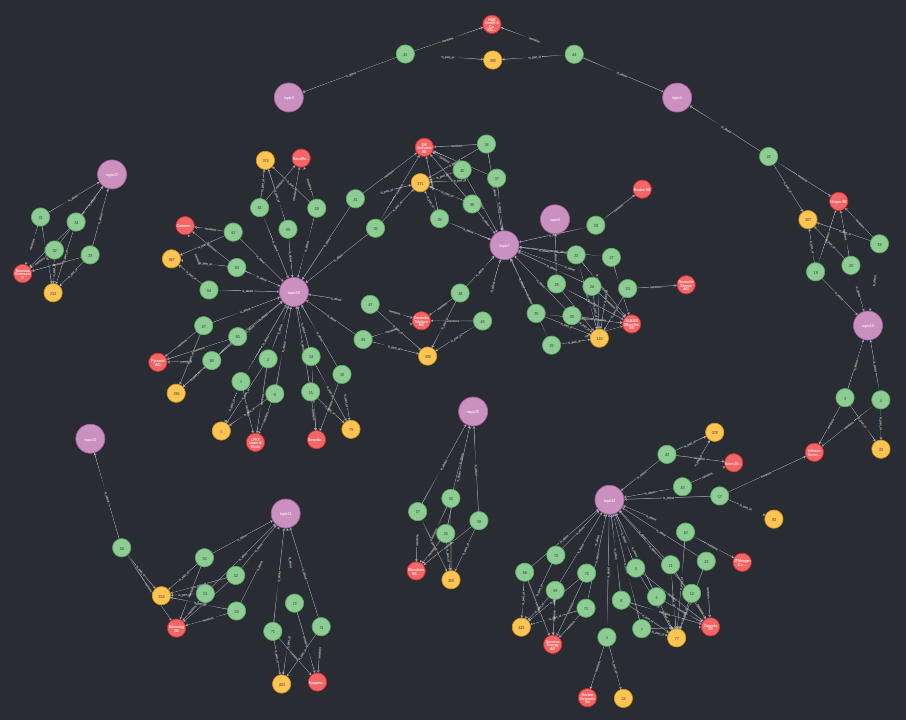
\includegraphics[width=1.0\textwidth]{Assets/kg-data-1}
    \caption{Knowledge Graph after Data Loading}
    \label{fig:kg-data-1}
\end{figure}

Zooming into an exemplary and disconnected Sub-Graph reveals some Relationships and Node properties, see Figure \ref{fig:kg-data-2}:

\begin{figure}[H]   %[h] puts picture right here. 't' stands for to, 'b' stands for bottom
    \centering
    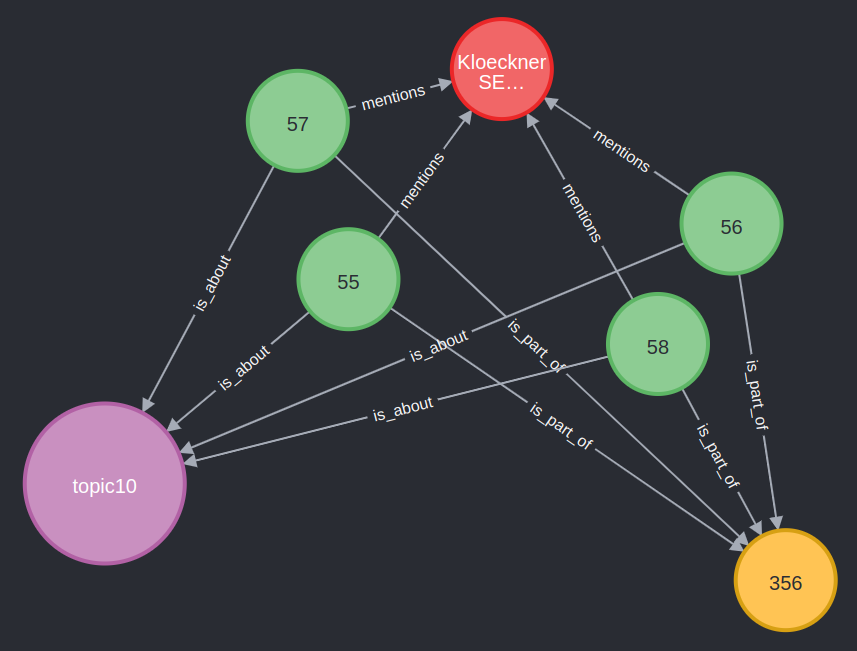
\includegraphics[width=1.0\textwidth]{Assets/kg-data-2}
    \caption{Exemplary, Disconnected Sub-Graph}
    \label{fig:kg-data-2}
\end{figure}

In the Sub-Graph (Fig.\ref{fig:kg-data-2}), a pink \emph{Topic} Node with its \emph{top\_id},
four green \emph{Sentence} Nodes with their \emph{sent\_id},
a yellow \emph{Article} Node with its \emph{art\_id} and
a red \emph{Company} Node with its \emph{comp\_name} properties are displayed.

The information for each Node can be displayed individually once they are selected in the browser:

\begin{figure}[H]
        \centering
        \begin{subfigure}[b]{0.475\textwidth}
            \centering
            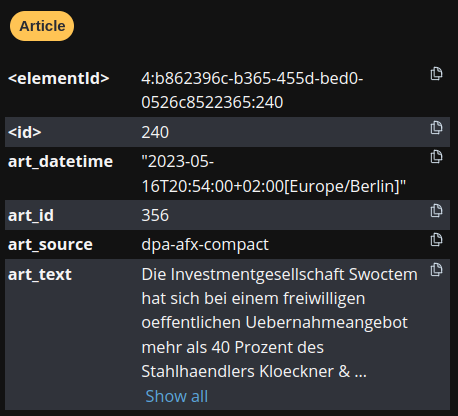
\includegraphics[width=\textwidth]{Assets/kg-data-3-article}
            \caption{\small Article}
            \label{fig:kg-data-3-article}
        \end{subfigure}
        \hfill
        \begin{subfigure}[b]{0.475\textwidth}
            \centering
            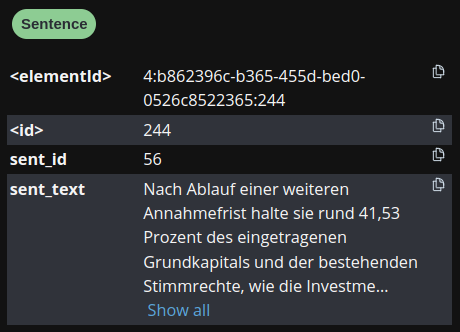
\includegraphics[width=\textwidth]{Assets/kg-data-3-sentence}
            \caption{\small Sentence}
            \label{fig:kg-data-3-sentence}
        \end{subfigure}
        \vskip\baselineskip
        \begin{subfigure}[b]{0.475\textwidth}
            \centering
            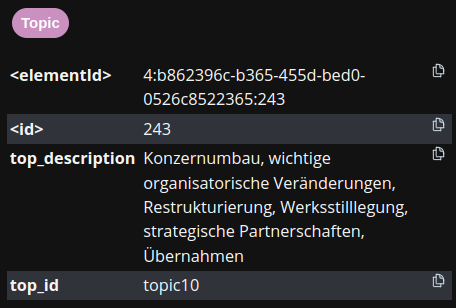
\includegraphics[width=\textwidth]{Assets/kg-data-3-topic}
            \caption{\small Topic}
            \label{fig:kg-data-3-topic}
        \end{subfigure}
        \hfill
        \begin{subfigure}[b]{0.475\textwidth}
            \centering
            \includegraphics[width=\textwidth]{Assets/kg-data-3-company}
            \caption{\small Company}
            \label{fig:kg-data-3-company}
        \end{subfigure}
        \caption{\small neo4j: Nodes and their Properties}
        \label{fig:nodes-and-props}
\end{figure}

The four boxes in Figure \ref{fig:nodes-and-props} show the Node properties for the respective \emph{Nodes} that were previously loaded.

\section{External Data}
Publicly accessible triple stores \cite{triple-store}, such as DBPedia \cite{dbpedia} or WikiData \cite{wikidata}, can be used to enrich the Knowledge Graph with external data.
For external data to be added to the existing Knowledge Graph, a unique and common identifier that exists in these triple stores, is necessary.
The previously discussed \gls{isin}, that was mapped from the Company Symbol (see Section \ref{par:symbol-isin}), is such an identifier.
The \emph{import\_wikidata\_id()} function in Python-Code \ref{code:import-wikidata-id} uses the \gls{isin} to retrieve the \emph{Wikidata entity id} \cite{wiki-entity-id} for each of the companies in the Knowledge Graph.

\begin{listing}[H]
    \captionof{listing}{Function: import\_wikidata\_id()}
    \inputminted[
    firstline=84,
    lastline=114,
    firstnumber=84,
    ]{python}{/media/rainergo/PROJECTS/UASFRA-MS-Thesis/src/F_knowledge_graph/B_graph_construction.py}
    \label{code:import-wikidata-id}
\end{listing}

\paragraph{SPARQL}
The function in lines 94-98 embeds a SPARQL \cite{sparql} query that is sent via an http-request to the Wikidata Query Service with the URL
\begin{center}
\emph{https://query.wikidata.org/sparql}
\end{center}
referenced in line 101.
SPARQL is a query language to query and retrieve stored RDF data such as Wikidata or DBPedia entities \cite{sparql}.
Wikidata and DBPedia are considered publicly available triple stores \cite{triple-store}.\\
neo4j's apoc \cite{neo4j-apoc} library processes the SPARQL response (lines 106-109) and inserts the \emph{wikidataID} into the respective property of each \emph{Company} Node, if the Wikidata entity page contains this information.\\

There are two other functions that can enrich the Knowledge Graph via SPARQL queries, namely
\emph{import\_data\_from\_wikidata()} and \emph{import\_data\_from\_dbpedia()}
in the \emph{GraphConstruction} class.
They can load any available information from triple stores that have a link to a \emph{Wikidata entity id} \cite{wiki-entity-id} or \gls{isin}.\\
To show some examples, I have used these functions to load the \emph{Industry} category, the home \emph{Country} and a short \emph{Abstract} about the companies
from Wikidata and DBPedia.
The respective SPARQL queries, that are automatically generated by the two functions, for demonstration purposes were manually composed and are shown in Figure \ref{fig:sparql-requests}.

\begin{figure}[H]
        \centering
        \begin{subfigure}[b]{0.80\textwidth}
            \centering
            \includegraphics[width=\textwidth]{Assets/wikirequest-indu}
            \caption{\small P452 - Industry}
            \label{fig:wikirequest-indu}
        \end{subfigure}
        \vskip\baselineskip
        \begin{subfigure}[b]{0.80\textwidth}
            \centering
            \includegraphics[width=\textwidth]{Assets/wikirequest-country}
            \caption{\small P17 - Country}
            \label{fig:wikirequest-country}
        \end{subfigure}
        \vskip\baselineskip
        \begin{subfigure}[b]{0.55\textwidth}
            \centering
            \includegraphics[width=\textwidth]{Assets/dbpedia-request-abstract}
            \caption{\small dbo:abstract - Abstract}
            \label{fig:dbpedia-request-abstract}
        \end{subfigure}
        \caption{\small SPARQL: Queries to enrich Knowledge Graph}
        \label{fig:sparql-requests}
\end{figure}

In the neo4j Subgraph \ref{fig:kg-data-4-company}, the \emph{Company} Node properties for \emph{Kloeckner \& Co SE} now include the information
for \emph{Industry}, \emph{Country} and an \emph{Abstract}.

\begin{figure}[H]
	\centering
	\includegraphics[width=\textwidth]{Assets/kg-data-4-company}
	\caption{Company Node after Data Enrichment}
	\label{fig:kg-data-4-company}
\end{figure}


\section{Information Retrieval}
With the data from the DataFrame and from external sources loaded, the Knowledge Graph can now be queried to retrieve information.

\paragraph{\gls{cypher} Queries}
\gls{cypher} queries provide a visual way to reveal patterns and relationships by using a human-friendly ASCII-based type of syntax \cite{neo4j}.

\begin{center}
    \textbf{(:nodes) - [:ARE\_CONNECTED\_TO] → (:otherNodes)}
\end{center}

Round brackets are used to represent \emph{(:Nodes)}, and \emph{-[:ARROWS]→} to represent a relationship between the \emph{(:Nodes)}.
\gls{cypher} queries can be used to reveal a wide range of Knowledge Graph information ranging from simple property values to complex, multi-hop relations.\\
A user, for instance, could be interested in news articles about a particular company such as \emph{Brenntag SE} or all companies that are mentioned in sentences about \emph{Topic12} on a specific day and so would compose the following Cyper queries:

\begin{figure}[H]
        \centering
        \begin{subfigure}[b]{\textwidth}
            \centering
            \includegraphics[width=\textwidth]{Assets/cypher-1}
            \caption{\small Cypher Query 1: Articles about \emph{Brenntag SE}}
            \label{fig:cypher-1}
        \end{subfigure}
        \vskip\baselineskip
        \begin{subfigure}[b]{\textwidth}
            \centering
            \includegraphics[width=\textwidth]{Assets/cypher-2}
            \caption{\small Cypher Query 2: Companies, Sentences about \emph{Topic12}}
            \label{fig:cypher-2}
        \end{subfigure}
        \caption{\small Cypher Queries 1-2}
        \label{fig:cypher-queries-pair1}
\end{figure}

Another user could be interested only in certain industry news for a particular day or only in sentences with certain topics and about companies that are located in Germany.
He could compile these \gls{cypher} queries:

\begin{figure}[H]
        \centering
        \begin{subfigure}[b]{\textwidth}
            \centering
            \includegraphics[width=\textwidth]{Assets/cypher-3}
            \caption{\small Cypher Query 3: Sentences about Industry \emph{Wholesale}}
            \label{fig:cypher-3}
        \end{subfigure}
        \vskip\baselineskip
        \begin{subfigure}[b]{\textwidth}
            \centering
            \includegraphics[width=\textwidth]{Assets/cypher-4}
            \caption{\small Cypher Query 4: German Companies, Sentences about Topic12}
            \label{fig:cypher-4}
        \end{subfigure}
        \caption{\small Cypher Queries 3-4}
        \label{fig:cypher-queries-pair2}
\end{figure}

The queries could be even more specific and nested and so reveal deep interrelations between \emph{Companies}, \emph{Articles}, \emph{Topics} and \emph{Sentences} and their particular properties.
The queries can be executed via the Python plugin or directly in the browser console and will be returned either as Graph visualization or as String in \gls{json} format.

\section{Sentence Embeddings and Sentiment}
So far, the \emph{Sentence} information is only stored as text in the Node's property \emph{sent\_text}.
But the \emph{Embedder} class in the \emph{F\_knowledge\_graph} directory allows to contextually embed (see Section \ref{subsec:contextual-word-embeddings}) these sentences.

The method \emph{create\_text\_embedding()} (Python-Code \ref{code:sent-text-embed}) in the previously cited \emph{GraphConstruction} class conveniently embeds all the sentences in the Knowledge Graph and
stores the embedding vector of size 768 in the new \emph{Sentence} Node property \emph{sent\_text\_embedding}:

\begin{listing}[H]
    \captionof{listing}{Function: create\_text\_embedding()}
    \inputminted[
    firstline=201,
    lastline=227,
    firstnumber=201,
    ]{python}{/media/rainergo/PROJECTS/UASFRA-MS-Thesis/src/F_knowledge_graph/B_graph_construction.py}
    \label{code:sent-text-embed}
\end{listing}
Once the function has run, each \emph{Sentence} text has been embedded and added to the \emph{Sentence} properties.
It again can be shown in the browser by selecting the respective \emph{Sentence} Node:

\begin{figure}[H]   %[h] puts picture right here. 't' stands for to, 'b' stands for bottom
    \centering
    \includegraphics[width=\textwidth]{Assets/sent-embed}
    \caption{BERT Sentence Embedding}
    \label{fig:sent-embed}
\end{figure}
As here a \gls{BERT} (\emph{bert-base-uncased}) model was used for the embeddings, the dimension of the embedding vector is 768.\\

With such sentence embeddings, it is possible to train a \emph{Sentiment Model} to classify these sentences into different categories.
For instance, a \emph{Sentiment Model} could be trained with three classes such as:

\begin{itemize}
    \item POSITIVE
    \item NEUTRAL
    \item NEGATIVE
\end{itemize}

Afterward, this model can predict the sentiment of all sentences based on their embeddings, and the respective \emph{Sentiment Class} would be added to the \emph{Sentence} Node properties.
\gls{cypher} queries could then retrieve and filter sentences with a certain sentiment.\\
A user who wanted to see
\begin{center}
\emph{"only NEGATIVE news sentences about German companies"}
\end{center}
could run the following exemplary \gls{cypher} query:

\begin{figure}[H]   %[h] puts picture right here. 't' stands for to, 'b' stands for bottom
    \centering
    \includegraphics[width=\textwidth]{Assets/sentiment}
    \caption{Sentence: Sentiment Classification}
    \label{fig:sentiment}
\end{figure}
Every such data enrichment of the Knowledge Graph, here the enrichment with sentence embeddings and sentiment classes, can enhance the Knowledge Graph's capability to retrieve complex information.

\section{\gls{graph-bot}}
The query language \gls{cypher} is relatively easy to learn and user-friendly, but not as friendly as the human language itself.\\
neo4j \cite{neo4j} via the LangChain \cite{LangChain} library offers a \emph{GraphCypherQAChain} and \emph{Neo4jGraph} module.
These modules, together with other LangChain components (see Section \ref{subsec:langchain-explain}), can be used to create a ChatBot that converts human language to \gls{cypher} queries, and \gls{cypher} responses back to human language.
This was done in the \emph{D\_graph\_bot.py} (Python-Codes \ref{code:chatbot-1} to \ref{code:chatbot-4}) module in the \emph{F\_knowledge\_graph} directory.

\begin{listing}[H]
    \captionof{listing}{Knowledge Graph Chatbot: init}
    \inputminted[
    firstline=70,
    lastline=82,
    firstnumber=70
    ]{python}{/media/rainergo/PROJECTS/UASFRA-MS-Thesis/src/F_knowledge_graph/D_graph_bot.py}
    \label{code:chatbot-1}
\end{listing}

The LangChain pipeline or chain uses an \gls{llm} (line 84 of Python-Code \ref{code:chatbot-1}) and explanatory Examples of which some are
shown in Python-Code \ref{code:chatbot-2}:

\begin{listing}[H]
    \captionof{listing}{Knowledge Graph Chatbot: Examples}
    \inputminted[
    firstline=14,
    lastline=35,
    firstnumber=14,
    fontsize=\tiny,
    ]{python}{/media/rainergo/PROJECTS/UASFRA-MS-Thesis/src/F_knowledge_graph/D_graph_bot.py}
    \label{code:chatbot-2}
\end{listing}
\begin{listing}[H]
    \captionof{listing}{Knowledge Graph Chatbot: \gls{prompt}}
    \inputminted[
    firstline=92,
    lastline=114,
    firstnumber=92,
     fontsize=\tiny,
    ]{python}{/media/rainergo/PROJECTS/UASFRA-MS-Thesis/src/F_knowledge_graph/D_graph_bot.py}
    \label{code:chatbot-3}
\end{listing}

These examples are then embedded into a \gls{prompt} (Python-Code \ref{code:chatbot-3}) which,
along the \emph{User Question}, is sent to the \gls{llm}, see Python-Code \ref{code:chatbot-4}:

\begin{listing}[H]
    \captionof{listing}{Knowledge Graph Chatbot: Request to \gls{llm}}
    \inputminted[
    firstline=122,
    lastline=131,
    firstnumber=122
    ]{python}{/media/rainergo/PROJECTS/UASFRA-MS-Thesis/src/F_knowledge_graph/D_graph_bot.py}
    \label{code:chatbot-4}
\end{listing}

An exemplary user that is interested in
\begin{center}
\emph{companies that were mentioned in sentences published between certain dates}
\end{center}
could pose text questions to the \gls{graph-bot} as shown in Python-Code \ref{code:chatbot-5}:

\begin{listing}[H]
    \captionof{listing}{\gls{graph-bot}: User Question}
    \inputminted[
    firstline=135,
    lastline=140,
    firstnumber=135
    ]{python}{/media/rainergo/PROJECTS/UASFRA-MS-Thesis/src/F_knowledge_graph/D_graph_bot.py}
    \label{code:chatbot-5}
\end{listing}

If the parameter \emph{verbose} (line 124 in Python-Code \ref{code:chatbot-4}) is set to \emph{True},
the \gls{graph-bot}'s processing steps will be displayed as depicted in Figures \ref{fig:chatbot-1} to \ref{fig:chatbot-3}:

\begin{figure}[H]   %[h] puts picture right here. 't' stands for to, 'b' stands for bottom
    \centering
    \includegraphics[width=\textwidth]{Assets/chatbot-question}
    \caption{\gls{graph-bot} - Part 1: Question}
    \label{fig:chatbot-1}
\end{figure}

After the user has sent his question to the \gls{graph-bot} (Fig. \ref{fig:chatbot-1}) ...
\begin{figure}[H]   %[h] puts picture right here. 't' stands for to, 'b' stands for bottom
    \centering
    \includegraphics[width=\textwidth]{Assets/chatbot-processing}
    \caption{\gls{graph-bot} - Part 2: Creating \gls{cypher} Queries}
    \label{fig:chatbot-2}
\end{figure}
... the \gls{graph-bot} converts this question into a corresponding \gls{cypher} query (Figure \ref{fig:chatbot-2}) and sends it to the neo4j graph database.

\begin{figure}[H]   %[h] puts picture right here. 't' stands for to, 'b' stands for bottom
    \centering
    \includegraphics[width=\textwidth]{Assets/chatbot-answer}
    \caption{\gls{graph-bot} - Part 3: Answer}
    \label{fig:chatbot-3}
\end{figure}

The JSON object returned by the neo4j graph database is then converted to human-readable text (Figure \ref{fig:chatbot-3}) and returned to the user.

\paragraph{\gls{graph-bot} vs. \gls{llm} Chatbot}
The \gls{graph-bot} is comparable to an \gls{llm} ChatBot such as ChatGPT in that a user can ask questions or \gls{prompt} the \gls{llm} ChatBot for specific tasks.
But they differ in that the \gls{graph-bot}'s answer is based on concrete text and factual data in news articles whereas the \gls{llm} ChatBot relies
on next-word probabilities.
Whereas the \gls{graph-bot} often returns the literal text of the existing news article in its answer (see Figure \ref{fig:chatbot-3}),
the \gls{llm} ChatBot returns newly generated text that might be contextually correct, but is often factually incorrect.

This lies in the nature of \gls{llm}s as they are trained to generalize well, but not to memorize the data they were trained with (as discussed in Section \ref{par:hallucination}).

Checking and validating the returned text from the \gls{llm} ChatBot is tedious and cumbersome,
whereas for the GraphBot, this can easily be done with \gls{cypher} queries.\\
In this sense, the \gls{graph-bot} is superior to a general \gls{llm} ChatBot if the user expects actual facts instead of newly generated text.


\paragraph{Production Use Case}
The \gls{graph-bot} currently only uses a few examples in its \gls{prompt} which are probably not enough to constantly get satisfactory
and correct answers.
For a production use case, the provided examples would need some enhancement and refinement.\\
Apart from this, the \gls{graph-bot} is a useful human interaction tool for users that do not want to write \gls{cypher} queries,
but use human language to retrieve information from the Knowledge Graph.


\paragraph{Knowledge Graph as RAG}
The Knowledge Graph served the \gls{graph-bot} as a data retriever and thus can be considered a \gls{RAG} system (see Section \ref{par:rag-systems}).
While typical RAG systems might distinguish documents with strongly different context, they usually suffer from the following shortcomings \cite{rag-cririque}:

\begin{itemize}
    \item Misunderstanding of documents that contain nuanced context differences.
    \item Chunking of document breaks its context.
    \item Vector database contains irrelevant information.
\end{itemize}

These issues are addressed by the Knowledge Graph in this project:
The \gls{gen-llm} in the Coreference Resolution and Topic Modelling pipeline could also semantically misunderstand the news article sentences,
but this is less likely as both pipeline components are tightly defined and accompanied by dedicated \gls{prompt} examples.
It was shown in the Topic Modelling section (see Section \ref{sec:topic-gen-llm}) that the \gls{gen-llm} component can indeed distinguish nuanced differences in context.
The relevant sentences are much shorter, more focused and less generic than typical documents in a vector database.
Both, the chunking and semantic interpretation is done on the sentence level so that the chunking cannot split the sentence's context \footnote{Under the assumption that sentence splitting works correctly}.
Each sentence with a found company is all relevant and thus cannot contain irrelevant information.\\
Thus, the vector database could be replaced by such a Knowledge Graph.
This is also supported by a recent research paper from Microsoft: GraphRAG \cite{graphrag}.
Instead of feeding the news article text to a vector database, it could be extracted and inserted into a Knowledge Graph, as it was shown in this project.




%\include{Chapters/Chapter_1}
%\chapter{Second Chapter}

\section{Section 1 Name}


\begin{minted}{python}
import numpy as np
    
def incmatrix(genl1,genl2):
    m = len(genl1)
    n = len(genl2)
    M = None #to become the incidence matrix
    VT = np.zeros((n*m,1), int)  #dummy variable
    
    #compute the bitwise xor matrix
    M1 = bitxormatrix(genl1)
    M2 = np.triu(bitxormatrix(genl2),1) 

    for i in range(m-1):
        for j in range(i+1, m):
            [r,c] = np.where(M2 == M1[i,j])
            for k in range(len(r)):
                VT[(i)*n + r[k]] = 1;
                VT[(i)*n + c[k]] = 1;
                VT[(j)*n + r[k]] = 1;
                VT[(j)*n + c[k]] = 1;
                
                if M is None:
                    M = np.copy(VT)
                else:
                    M = np.concatenate((M, VT), 1)
                
                VT = np.zeros((n*m,1), int)
    
    return M 
\end{minted}

\section{Section 2 Name}

% Importing code from Python file and overwrite global minted settings
\inputminted[
firstline=3,
lastline=9, 
firstnumber=3,
]{python}{Assets/test.py}
%\include{Chapters/Chapter_3_Pics}
%\chapter{Fourth Chapter}

\section{Section 1 Name}
I want to make a reference to the bibliography here\cite{Abc} and after that another text.

\section{Section 2 Name}
I want to make a footnote right here\footnote{This is my first footnote}

\section{Section 3 Name}
I want to make a footnote holder right here\footnotetext{This is my second footnote} to reference it later, for example in the next section.

\section{Section 4 Name}
Here\footnotemark{} is now my footnote that I marked before.
%\chapter{Math Formulas}\label{ch:math-formulas}
$$
\alpha
\beta
\gamma
\rho
\sigma
\delta
\epsilon
\times
\otimes
\oplus
\cup
\cap
\subset
\supset
\subseteq
\supseteq
\int
\oint
\sum
\prod
$$

$ E = mc^2 $

$$ 1+\frac{2}{4} $$



%------------------------------------------------------
%    CONTENT-OUTRO
%------------------------------------------------------
\chapter{Conclusion}

The goal of this Master-Thesis project was to extract structured information from unstructured text and store this information in a Knowledge Graph.\\

In this thesis and the accompanying Python code, it was shown how a predefined set of corporate entity names and their \glspl{coref_definition} can be found in financial news articles.
It was also shown, how sentences that contained this company information, were classified with a Topic model and stored in a Knowledge Graph.
In the \emph{Information Extraction Pipeline}, different approaches were studied, implemented in code and compared with each other.
It was learned, that \gls{gen-llm}s can be used for a wide range of extraction tasks and that these models often outperform other approaches.\\

The conversion of formerly unstructured text in files to structured data in a Knowledge Graph facilitates information retrieval.
Information that was previously stored in an inaccessible form can, after conversion, be more readily accessed through the use of structured \gls{cypher} queries or a \gls{graph-bot}.
The retrieved information from the Knowledge Graph should also be more accurate than the information coming from a \gls{gen-llm} ChatBot, even if the \gls{gen-llm} ChatBot has a typical \gls{RAG} system attached to it.
This is because the Knowledge Graph's response is more based on actual news articles and less on next-word probabilities.\\

As already mentioned, the few-shot examples provided to the \gls{coref_resolution_definition}, Topic Modelling and \gls{graph-bot} models, would need to be improved
in a production use case.
Given the more limited scope of a Master-Thesis and to present the process rather than the result, I nevertheless deem the state of the current models sufficient.\\

Evaluation of the different models was done by individually comparing their performance on some exemplary data.
The exemplary data was randomly sampled and might not represent the feature/data distribution of all scraped financial news articles or financial news articles in general very well.
The comparison of the different models was also done manually and individually without using common performance measurement metrics such as accuracy, precision or recall.
A key reason for this was the challenge of categorizing model prediction outcomes into clear binary classes of \emph{correct} and \emph{incorrect}
and the extensive nature of the performance evaluation process: each prediction from every component within the \emph{Information Extraction Pipeline} for each sentence would require manual assessment and verification.
In a production use case, a more thorough performance assessment was necessary.
But again: Given the more limited scope of a Master-Thesis, I nevertheless deem the model evaluation process sufficient.\\


In hindsight, I would approach some tasks differently.
The usage of a spacy pipeline was motivated by the initial assumption that pre-trained spacy pipelines were among the best-performing models.
This assumption must be abandoned, at least for the given data samples, as none of spacy's models or external plugins could compete with either \gls{gen-llm}s or other pre-trained models.
The \emph{Information Extraction Pipeline} could have been fully built without the spacy library.\\

I would also focus more on \gls{llm} frameworks such as LangChain \cite{LangChain}, LlamaIndex \cite{llamaindex} or DSPy \cite{dspy} and their ever-growing capabilities.
The usage of tools, agents and other innovative concepts and components could probably further improve the performance of \gls{gen-llm}s for all kinds of extraction tasks.\\








\appendix   % Resets enumeration from numerical to alphabetical enumeration
\chapter{Explanation of \textbf{MAIN.ipynb} file}\label{ch:explanation-of-main-file}

This is a short explanation about the Jupiter Notebook \emph{MAIN.ipynb} in the root directory of the project's repository.
The Notebook aggregates and condenses all functionalities of the Python code.

\begin{figure}[H]   %[h] puts picture right here. 't' stands for to, 'b' stands for bottom
    \centering
    \includegraphics[width=0.95\textwidth]{Assets/main-1}
    \caption{STEP 1: Import libraries}
    \label{fig:main-1}
\end{figure}

\begin{figure}[H]   %[h] puts picture right here. 't' stands for to, 'b' stands for bottom
    \centering
    \includegraphics[width=0.95\textwidth]{Assets/main-2}
    \caption{STEP 2: Start Docker container}
    \label{fig:main-2}
\end{figure}
\begin{figure}[H]   %[h] puts picture right here. 't' stands for to, 'b' stands for bottom
    \centering
    \includegraphics[width=0.95\textwidth]{Assets/main-3}
    \caption{STEP 3: Load News Articles}
    \label{fig:main-3}
\end{figure}
\begin{figure}[H]   %[h] puts picture right here. 't' stands for to, 'b' stands for bottom
    \centering
    \includegraphics[width=0.95\textwidth]{Assets/main-4}
    \caption{STEP 4: Run spacy pipeline (NER, COREF)}
    \label{fig:main-4}
\end{figure}
\begin{figure}[H]   %[h] puts picture right here. 't' stands for to, 'b' stands for bottom
    \centering
    \includegraphics[width=0.95\textwidth]{Assets/main-5}
    \caption{STEP 5: Convert Nested Dictionary}
    \label{fig:main-5}
\end{figure}
\begin{figure}[H]   %[h] puts picture right here. 't' stands for to, 'b' stands for bottom
    \centering
    \includegraphics[width=0.95\textwidth]{Assets/main-6}
    \caption{STEP 6: Start Topic Modelling Process}
    \label{fig:main-6}
\end{figure}
\begin{figure}[H]   %[h] puts picture right here. 't' stands for to, 'b' stands for bottom
    \centering
    \includegraphics[width=0.95\textwidth]{Assets/main-7}
    \caption{STEP 7: Prepare DataFrame for Knowledge Graph}
    \label{fig:main-7}
\end{figure}
\begin{figure}[H]   %[h] puts picture right here. 't' stands for to, 'b' stands for bottom
    \centering
    \includegraphics[width=0.95\textwidth]{Assets/main-8}
    \caption{STEP 8: Initialize Knowledge Graph and load Data}
    \label{fig:main-8}
\end{figure}
\begin{figure}[H]   %[h] puts picture right here. 't' stands for to, 'b' stands for bottom
    \centering
    \includegraphics[width=0.95\textwidth]{Assets/main-9}
    \caption{STEP 9: Enrich Knowledge Graph with Data from Wikidata}
    \label{fig:main-9}
\end{figure}
\begin{figure}[H]   %[h] puts picture right here. 't' stands for to, 'b' stands for bottom
    \centering
    \includegraphics[width=0.95\textwidth]{Assets/main-10}
    \caption{STEP 10: Enrich Knowledge Graph with Data from DBPedia}
    \label{fig:main-10}
\end{figure}
\begin{figure}[H]   %[h] puts picture right here. 't' stands for to, 'b' stands for bottom
    \centering
    \includegraphics[width=0.95\textwidth]{Assets/main-11}
    \caption{STEP 11: Create Sentence Text Embeddings}
    \label{fig:main-11}
\end{figure}
\begin{figure}[H]   %[h] puts picture right here. 't' stands for to, 'b' stands for bottom
    \centering
    \includegraphics[width=0.95\textwidth]{Assets/main-12}
    \caption{STEP 12: Communicate with Graph Bot}
    \label{fig:main-12}
\end{figure}

%\include{Chapters/MAIN2}
\listoffigures
%\printnoidxglossaries

%------------------------------------------------------
%    BIBLIOGRAPHY
%------------------------------------------------------
\bibliographystyle{plain}
\bibliography{bibliography}

\end{document}
